\باب{ماورائی تفاعل}
وہ تفاعل \عددی{y=f(x)} جو درج ذیل روپ کی مساوات کو مطمئن کرتا ہو \اصطلاح{الجبرائی}\فرہنگ{الجبرائی}\حاشیہب{algebraic}\فرہنگ{algebraic} کہلاتا ہے۔
\begin{align*}
P_ny^n+\cdots+P_1y+P_0=0
\end{align*}
اس مساوات میں تمام \عددی{P} متغیر \عددی{x} کے کثیر رکنی ہیں جہاں کثیر رکنیوں کے عددی سر ناطق ہیں۔ یوں \عددی{y=\tfrac{1}{\sqrt{x+1}}} الجبرائی ہے چونکہ یہ مساوات \عددی{(x+1)y^2-1=0} کو مطمئن کرتا ہے جس میں \عددی{P_2=x+1}، \عددی{P_1=0} اور \عددی{P_0=-1} ہیں۔ کثیر رکنی اور ناطق عددی سر والے ناطق تفاعل، الجبرائی ہوں گے۔اسی طرح الجبرائی تفاعل کے مجموعے، حاصل ضرب، حاصل تقسیم، ناطق طاقت اور ناطق جذر بھی الجبرائی ہوں گے۔

وہ تفاعل جو الجبرائی نہیں ہوں \اصطلاح{ماورائی}\فرہنگ{ماورائی}\حاشیہب{transcendental}\فرہنگ{transcendental} کہلاتے ہیں۔ چھ بنیادی تکونیاتی تفاعل \عددی{\sin}، \عددی{\cos}، \عددی{\tan}، \عددی{\csc}، \عددی{\sec}، \عددی{\cot} اور ان کے الٹ ماورائی ہیں۔ اسی طرح قوت نمائی تفاعل اور لوگارتھمی تفاعل بھی ماورائی تفاعل ہیں۔

وہ اعداد جو ناطق عددی سر والے کثیر رکنی مساوات کو مطمئن کرتے ہوں \اصطلاح{الجبرائی} کہلاتے ہیں۔چونکہ \عددی{-2} مساوات \عددی{x+2=0} کو مطمئن کرتا ہے لہٰذا \عددی{-2} الجبرائی عدد ہے۔ اسی طرح \عددی{x^2-3=0} کو \عددی{\sqrt{3}} مطمئن کرتا ہے لہٰذا \عددی{\sqrt{3}} بھی الجبرائی عدد ہے۔ وہ اعداد جو الجبرائی نہ ہوں \اصطلاح{ماورائی} کہلاتے ہیں۔ \عددی{e} اور \عددی{\pi} ماورائی اعداد ہیں۔

  ریاضیات میں بہت سے تفاعل ایک دوسرے کے الٹ ہیں۔ غالباً سب سے زیادہ جانی پہچانی الٹ تفاعل کی جوڑی \عددی{\ln x} اور \عددی{e^x} ہے۔ موزوں وقفہ پر پابند تکونیاتی تفاعل کے اہم الٹ پائے  جاتے ہیں۔ اسی طرح  لوگارتھمی اور قوت نمائی تفاعل کے دیگر الٹ جوڑیاں پائی جاتی ہیں۔ ہذلولی تفاعل اور ان کے الٹ تفاعل کا استعمال آویزاں رسی، منتقلی حرکی توانائی، اور ہوا میں گرتے ہوئے جسم پر قوت رگڑ کے مسائل میں کام آتے ہیں۔ اس باب میں ان تمام تفاعل پر غور کیا جائے گا۔ ان مسئلوں کا بھی ذکر کیا جائے گا جنہیں یہ تفاعل حل کرنے میں مدد گار ثابت ہوتے ہیں۔

\حصہ{الٹ تفاعل اور ان کے تفرق}
اس حصہ میں ہم الٹ تفاعل کی تعریف پیش کرتے ہیں اور ان کی کلیات، ترسیمات، اور الٹ جوڑیوں کے تفرق پر غور کرتے ہیں۔

\جزوحصہء{ایک ایک تفاعل}
تفاعل سے مراد وہ قاعدہ ہے جو اپنی دائرہ کار کے ہر نقطہ کو اپنی سعت میں ایک قیمت مختص کرتا ہو۔بعض تفاعل ایک ہی قیمت کو ایک سے زیادہ  نقطوں  کے لئے مختص کرتے ہیں۔ یوں \عددی{-1} کا مربع اور \عددی{1} کا مربع \عددی{1} ہے؛ اسی طرح \عددی{\tfrac{\pi}{3}} اور \عددی{\tfrac{2\pi}{3}} کا سائن \عددی{\tfrac{\sqrt{3}}{2}} ہے۔ اس کے بر عکس دیگر تفاعل کسی ایک قیمت کو کبھی بھی دو بار مختص نہیں کرتے ہیں۔ مختلف اعداد کے جذر المربع اور جذر الکعب ہر صورت ایک دوسرے سے مختلف ہوتے ہیں۔ ایسا تفاعل جس کے انفرادی نقطوں پر منفرد قیمت ہو کو \اصطلاح{ایک ایک تفاعل}\فرہنگ{ایک ایک تفاعل}\حاشیہب{one to one function}\فرہنگ{one to one} کہتے ہیں۔

\ابتدا{تعریف}
دائرہ کار \عددی{D} پر تفاعل \عددی{f(x)}  تب \اصطلاح{ایک ایک} ہو گا جب \عددی{x_1\ne x_2} کی صورت میں \عددی{f(x_1)\ne f(x_2)} ہو۔
\انتہا{تعریف}
%=====================

\ابتدا{مثال}
چونکہ کسی بھی غیر منفی اعداد کے لئے \عددی{x_1\ne x_2} کی صورت میں \عددی{\sqrt{x_1}\ne \sqrt{x_2}} ہے  لہٰذا \عددی{f(x)=\sqrt{x}} غیر منفی اعداد کے کسی بھی دائرہ کار پر یہ ایک ایک تفاعل ہے۔
\انتہا{مثال}
%====================
\ابتدا{مثال}
چونکہ \عددی{\sin(\tfrac{\pi}{6})=\sin(\tfrac{5\pi}{6})} ہے لہٰذا وقفہ \عددی{[0,\pi]} پر \عددی{g(x)=\sin x} ایک ایک تفاعل نہیں ہے۔ اس کے برعکس چونکہ ربع اول میں تمام زاویوں کے سائن مختلف ہیں لہٰذا وقفہ \عددی{[0,\tfrac{\pi}{2}]} پر \عددی{g(x)=\sin x} ایک ایک تفاعل ہے۔
\انتہا{مثال}
%====================
\begin{figure}
\centering
\begin{subfigure}{0.45\textwidth}
\centering
\begin{tikzpicture}[declare function={f(\x)=\x^3;g(\x)=sqrt{\x};}]
\begin{axis}[clip=false,small,axis lines=middle,enlargelimits=true,xlabel={$x$},ylabel={$y$},xlabel style={at={(current axis.right of origin)},anchor=west},ylabel style={at={(current axis.above origin)},anchor=south},xtick={\empty},ytick={\empty}]
\addplot[domain=0:1.2]{f(x)}node[right]{$y=x^3$};
\addplot[domain=0:1.2](-x,{-f(x)});
\draw(-1.2,1)--(1.2,1);
\end{axis}
\end{tikzpicture}
\caption{ایک ایک تفاعل۔}
\end{subfigure}\hfill
\begin{subfigure}{0.45\textwidth}
\centering
\begin{tikzpicture}[declare function={f(\x)=\x^3;g(\x)=sqrt{\x};}]
\begin{axis}[clip=false,small,axis lines=middle,enlargelimits=true,xlabel={$x$},ylabel={$y$},xlabel style={at={(current axis.right of origin)},anchor=west},ylabel style={at={(current axis.above origin)},anchor=south},xtick={\empty},ytick={\empty}]
\addplot[domain=0:0.5]{g(x)};
\addplot[domain=0.5:2]{g(x)}node[right]{$y=\sqrt{x}$};
\draw(-0.25,1)--(2,1);
\end{axis}
\end{tikzpicture}
\caption{ایک ایک تفاعل۔}
\end{subfigure}
\begin{subfigure}{0.45\textwidth}
\centering
\begin{tikzpicture}[font=\small,declare function={f(\x)=\x^2;g(\x)=sin(deg(\x));}]
\begin{axis}[clip=false,small,axis lines=middle,enlargelimits=true,xlabel={$x$},ylabel={$y$},xlabel style={at={(current axis.right of origin)},anchor=west},ylabel style={at={(current axis.above origin)},anchor=south},xtick={\empty},ytick={\empty}]
\addplot[domain=-1.25:1.25]{f(x)}node[right]{$y=x^2$};
\draw(-1.25,1)--(1.25,1);
\draw[dashed](-1,1)--(-1,0)node[below]{$-1$};
\draw[dashed](1,1)--(1,0)node[below]{$1$};
\draw[](0,1)node[above left]{$1$};
\draw(-1+0.02,1.02)--(-0.25,1.25);
\draw(1-0.02,1.02)--(0.25,1.25);
\draw(0,1.25)node[above,fill=white]{\RL{$y$ کی قیمتیں ایک جیسی ہیں}};
\end{axis}
\end{tikzpicture}
\caption{غیر ایک ایک تفاعل۔}
\end{subfigure}\hfill
\begin{subfigure}{0.45\textwidth}
\centering
\begin{tikzpicture}[font=\small,declare function={f(\x)=\x^2;g(\x)=sin(deg(\x));}]
\pgfmathsetmacro{\a}{pi/6}
\pgfmathsetmacro{\b}{5/6*pi}
\begin{axis}[clip=false,small,axis lines=middle,enlargelimits=true,xlabel={$x$},ylabel={$y$},xlabel style={at={(current axis.right of origin)},anchor=west},ylabel style={at={(current axis.above origin)},anchor=south},xtick={\empty},ytick={\empty}]
\addplot[domain=-0.2:3.3]{g(x)}node[pos=0.5,above]{$y=\sin x$};
\draw(-0.25,0.5)--(3.3,0.5);
\draw[dashed](\a,0.5)--(\a,0)node[below]{$\tfrac{\pi}{6}$} (\b,0.5)--(\b,0)node[below]{$\tfrac{5\pi}{6}$};
\draw(0,0.5)node[above left]{$0.5$};
\draw(\a+0.02,{g(\a)-0.02})--(\a+0.5,0.2);
\draw(\b-0.02,{g(\b)-0.02})--(\b-0.5,0.2);
\draw({1/2*(\a+\b)},0.3)node[below,fill=white]{\RL{$y$ کی قیمتیں ایک جیسی ہیں}};
\end{axis}
\end{tikzpicture}
\caption{غیر ایک ایک تفاعل۔}
\end{subfigure}
\caption{ایک ایک تفاعل کی ترسیم کسی بھی افقی لکیر کو زیادہ سے زیادہ ایک بار قطع کرتی ہے جبکہ غیر ایک ایک تفاعل کی ترسیم، ایک یا ایک سے زیادہ افقی لکیروں کو ایک سے زیادہ بار قطع کرتی ہے۔}
\label{شکل_ماورائی_ایک_ایک_تفاعل_افقی_لکیر_پرکھ}
\end{figure}
ایک ایک تفاعل \عددی{y=f(x)} کی ترسیم کسی بھی افقی لکیر کو زیادہ سے زیادہ ایک بار قطع کرتی ہے ۔ اگر کسی تفاعل کی ترسیم کسی افقی لکیر کو ایک سے زیادہ مرتبہ قطع کرتی ہو تب یہ تفاعل \عددی{y} کی اس قیمت کو ایک سے زیادہ مرتبہ اختیار کرتا ہے لہٰذا یہ ایک ایک تفاعل نہیں ہو گا (شکل \حوالہ{شکل_ماورائی_ایک_ایک_تفاعل_افقی_لکیر_پرکھ})۔

\موٹا{افقی لکیر کا پرکھ}\\
کوئی بھی تفاعل \عددی{y=f(x)} صرف اور صرف اس صورت ایک ایک تفاعل ہو گا جب اس کی ترسیم ہر افقی لکیر کو زیادہ سے زیادہ ایک بار قطع کرتی ہو۔ 

\جزوحصہء{الٹ}
چونکہ ایک ایک تفاعل کا ہر مخارج  انفرادی مداخل  سے آتا ہے لہٰذا ایک ایک تفاعل کو الٹ کرتے ہوئے ہر مخارج کو واپس اس مداخل پر بھیجا جا سکتا ہے جس سے یہ مخارج حاصل ہوتا ہے (شکل \حوالہ{شکل_ماورائی_الٹ_واپس_بھیجتا_ہے})۔ ایک ایک تفاعل \عددی{f} کو الٹ کر کے جو تفاعل حاصل ہوتا ہے اس کو \عددی{f} کا \اصطلاح{الٹ}\فرہنگ{الٹ}\حاشیہب{inverse}\فرہنگ{inverse} کہتے ہیں جس کو \عددی{f^{-1}} سے ظاہر کیا جاتا ہے جہاں \عددی{f^{-1}} میں \عددی{-1} کو طاقت نہ سمجھا جائے: یعنی \عددی{f(x)^{-1}} سے مراد \عددی{\tfrac{1}{f(x)}} نہیں ہے۔ ہم \عددی{f^{-1}} کو "\عددی{f} کا الٹ" پڑھتے ہیں۔
\begin{figure}
\centering
\begin{tikzpicture}
\pgfmathsetmacro{\r}{1}
\draw(0,0) circle (\r);
\draw(3,0) circle (\r);
\draw(0,0)node[circ]{}node[left]{$x$}node[inner sep=0.3mm](kL){};
\draw(3,0)node[circ]{}node[right]{$y$}node[inner sep=0.3mm](kR){};
\draw[-stealth](kL) to [out=30,in=150]node[pos=0.5,above]{$f$}(kR);
\draw[-stealth](kR) to [out=-150,in=-30]node[pos=0.5,below]{$f^{-1}$}(kL);
\draw(0,\r)node[above]{\RL{$f$ کا دائرہ کار}};
\draw(3,\r)node[above]{\RL{$f$ کی سعت}};
\draw(0,-\r)node[below]{\RL{$f^{-1}$ کی سعت}};
\draw(3,-\r)node[below]{\RL{$f^{-1}$ کا دائرہ کار}};
\draw(-\r,0)node[left]{$x=f^{-1}(y)$};
\draw(3+\r,0)node[right]{$y=f(x)$};
\end{tikzpicture}
\caption{
تفاعل \عددی{f} کا الٹ ہر مخارج کو واپس اس مداخل پر بھیجتا ہے جہاں سے وہ آیا و۔
}
\label{شکل_ماورائی_الٹ_واپس_بھیجتا_ہے}
\end{figure}

جیسا شکل \حوالہ{شکل_ماورائی_الٹ_واپس_بھیجتا_ہے} سے ظاہر ہے، \عددی{f} سے \عددی{f^{-1}} یا \عددی{f^{-1}} سے \عددی{f} حاصل کیا جا سکتا ہے۔ یوں کسی بھی \عددی{x} کے لئے \عددی{f(x)} حاصل کر کے اس \عددی{f(x)} کا الٹ \عددی{f^{-1}(f(x))} حاصل کیا جا سکتا ہے جو \عددی{x} ہو گا۔ تفاعل \عددی{f^{-1}(f(x))} یا تفاعل \عددی{f(f^{-1}(x))} میں \عددی{x} پر کرنے سے واپس \عددی{x} ملتا ہے۔ ایسا تفاعل جو ہر عدد کو اسی عدد کے لئے مختص کرتا ہو  \اصطلاح{شناختی تفاعل}\فرہنگ{شناختی تفاعل}\فرہنگ{تفاعل!شناختی}\حاشیہب{identity function}\فرہنگ{identity function}\فرہنگ{function!identity} کہلاتا ہے۔ یوں تفاعل \عددی{f} اور \عددی{g} کو ایک دوسرے  کا الٹ تفاعل ہونے کے لئے پرکھا جا سکتا ہے۔اگر \عددی{(f\circ g)(x)=(g\circ f)(x)=x} ہو تب \عددی{f} اور \عددی{g} ایک دوسرے کے الٹ تفاعل ہوں گے ورنہ یہ ایک دوسرے کے الٹ تفاعل نہیں ہوں گے۔ اگر \عددی{f} اپنے دائرہ کار کا مکعب لیتا ہو تب \عددی{g} اس صورت \عددی{f} کا الٹ ہو گا اگر \عددی{g} جذر الکعب لیتا ہو ورنہ یہ \عددی{f} کا الٹ نہیں ہو گا۔

تفاعل \عددی{f} اور \عددی{g} ایک دوسرے کے الٹ صرف اور صرف اس صورت ہوں گے جب
\begin{align*}
f(g(x))=x\quad \text{اور}\quad g(f(x))=x
\end{align*}
ہوں۔ایسی صورت میں \عددی{g=f^{-1}} اور \عددی{f=g^{-1}} ہوں گے۔

ایک تفاعل کا الٹ صرف اور صرف اس صورت ہو گا جب یہ ایک ایک تفاعل ہو۔ یوں بڑھتے تفاعل کا الٹ تفاعل ہو گا اور  گھٹتے تفاعل کا بھی الٹ تفاعل ہو گا۔ جن تفاعل کا تفرق مثبت ہو وہ اپنے دائرہ کار میں بڑھتے ہیں لہٰذا ان کا الٹ ہو گا (صفحہ \حوالہصفحہ{نتیجہ_صریح_استعمال_سوم} پر مسئلہ اوسط قیمت کا ضمنی نتیجہ \حوالہ{نتیجہ_صریح_استعمال_سوم})۔اسی طرح جن تفاعل کا تفرق منفی ہو وہ اپنے دائرہ کار میں گھٹتے ہیں لہٰذا ان کا الٹ ہو گا۔
\begin{figure}
\centering
\begin{subfigure}{0.45\textwidth}
\centering
\begin{tikzpicture}[declare function={f(\x)=(\x+1)^(1/3);g(\x)=\x^3-1;}]
\begin{axis}[clip=false,small,axis lines=middle,enlargelimits=true,xlabel={$x$},ylabel={$y$},xlabel style={at={(current axis.right of origin)},anchor=west},ylabel style={at={(current axis.above origin)},anchor=south},xtick={\empty},ytick={\empty}, xmin=-1.25, xmax=3.5, ymin=-1.25, ymax=2.25]
%\addplot[domain=0:1.5]{g(x)};
\addplot[domain=-1:-0.8]{f(x)};
\addplot[domain=-0.8:3]{f(x)}node[below]{$y=f(x)$};
\draw(1.5,0)node[below,yshift=-2ex]{\RL{$f$ کا دائرہ کار}};
\draw(0,{f(1.5)})node[rotate=90,above,yshift=2ex]{\RL{$f$ کی سعت}};
\draw[-stealth](1.5,0)node[below]{$x$}--(1.5,{f(1.5)});
\draw[-stealth](1.5,{f(1.5)})--(0,{f(1.5)})node[left]{$y$};
\end{axis}
\end{tikzpicture}
\caption{
نقطہ \عددی{x} پر \عددی{f} کی قیمت جاننے کے لئے ہم \عددی{x} سے انتصابی رخ چلتے ہوئے ترسیم تک پہنچ کر افقی سمت محور \عددی{y} تک پہنچ کر درکار قیمت پڑھتے ہیں۔
}
\end{subfigure}\hfill
\begin{subfigure}{0.45\textwidth}
\centering
\begin{tikzpicture}[declare function={f(\x)=(\x+1)^(1/3);g(\x)=\x^3-1;}]
\begin{axis}[clip=false,small,axis lines=middle,enlargelimits=true,xlabel={$x$},ylabel={$y$},xlabel style={at={(current axis.right of origin)},anchor=west},ylabel style={at={(current axis.above origin)},anchor=south},xtick={\empty},ytick={\empty}, xmin=-1.25, xmax=3.5, ymin=-1.25, ymax=2.25]
%\addplot[domain=0:1.5]{g(x)};
\addplot[domain=-1:-0.8]{f(x)};
\addplot[domain=-0.8:3]{f(x)}node[below]{$x=f^{-1}(y)$};
\draw(1.5,0)node[below,yshift=-2ex]{\RL{$f^{-1}$ کی سعت}};
\draw(0,{f(1.5)})node[rotate=90,above,yshift=2ex,xshift=1ex]{\RL{$f^{-1}$ کا دائرہ کار}};
\draw[stealth-](1.5,0)node[below]{$x$}--(1.5,{f(1.5)});
\draw[stealth-](1.5,{f(1.5)})--(0,{f(1.5)})node[left]{$y$};
\end{axis}
\end{tikzpicture}
\caption{}
تفاعل \عددی{f} کی ترسیم کو \عددی{f^{-1}} کی ترسیم تصور کیا جا سکتا ہے۔ وہ \عددی{x} جو \عددی{y} دیتا ہو کو تلاش کرنے کی خاطر، ہم  \عددی{y} سے افقی رخ  ترسیم تک اور پھر انتصابی رخ محور \عددی{x} تک پہنچ کر درکار \عددی{x} پڑھتے ہیں۔ \عددی{f} کا دائرہ کار \عددی{f^{-1}} کی سعت ہو گی جبکہ \عددی{f} کی سعت \عددی{f^{-1}} کا دائرہ کار ہو گا۔

\end{subfigure}
\begin{subfigure}{0.45\textwidth}
\centering
\begin{tikzpicture}[declare function={f(\x)=(\x+1)^(1/3);g(\x)=\x^3-1;}]
\pgfmathsetmacro{\b}{1.15}
\pgfmathsetmacro{\a}{g(\b)}
\begin{axis}[clip=false,small,axis lines=middle,enlargelimits=true,xlabel={$x$},ylabel={$y$},xlabel style={at={(current axis.right of origin)},anchor=west},ylabel style={at={(current axis.above origin)},anchor=south},xtick={\empty},ytick={\empty}, xmin=-1.25, xmax=3.5, ymin=-1.25, ymax=2.25]
\addplot[domain=0:1.5]{g(x)}node[above]{$x=f^{-1}(y)$};
\addplot[gray,domain=-1:-0.8]{f(x)};
\addplot[gray,domain=-0.8:3]{f(x)};
\draw(1.5,0)node[below,xshift=2ex,yshift=-2ex]{\RL{$f^{-1}$ کا دائرہ کار}};
\draw(0,1.75)node[rotate=90,above]{\RL{$f^{-1}$ کی سعت}};
\draw[](\b,\a)node[circ]{}node[right]{$(b,a)$};
\draw[gray](\a,\b)node[circ]{}node[above]{$(a,b)$};
\draw[dashed](-1,-1)--(2.25,2.2)node[right]{$y=x$};
\end{axis}
\end{tikzpicture}
\caption{
تفاعل \عددی{f^{-1}} کو ترسیم  کرنے کی خاطر ہم \عددی{f} کا لکیر \عددی{y=x} میں عکس لیتے ہیں۔ 
}
\end{subfigure}\hfill
\begin{subfigure}{0.45\textwidth}
\centering
\begin{tikzpicture}[declare function={f(\x)=(\x+1)^(1/3);g(\x)=\x^3-1;}]
\begin{axis}[clip=false,small,axis lines=middle,enlargelimits=true,xlabel={$x$},ylabel={$y$},xlabel style={at={(current axis.right of origin)},anchor=west},ylabel style={at={(current axis.above origin)},anchor=south},xtick={\empty},ytick={\empty}, xmin=-1.25, xmax=3.5, ymin=-1.25, ymax=2.25]
\addplot[domain=0:1.5]{g(x)}node[pos=0.75,right]{$y=f^{-1}(x)$};
%\addplot[domain=-1:-0.8]{f(x)};
%\addplot[domain=-0.8:3]{f(x)}node[below]{$x=f^{-1}(y)$};
\draw(1.5,0)node[below,xshift=2ex,yshift=-2ex]{\RL{$f^{-1}$ کا دائرہ کار}};
\draw(0,1.75)node[rotate=90,above]{\RL{$f^{-1}$ کی سعت}};
\end{axis}
\end{tikzpicture}
\caption{
آخر میں ہم حرف \عددی{x} اور حرف \عددی{y} کا آپس میں تبادلہ  کرتے ہیں۔ یوں متغیر \عددی{x} کے تفاعل \عددی{f^{-1}} کی ترسیم حاصل ہوتی ہے۔ 
}
\end{subfigure}
\caption{تفاعل \عددی{f} کے الٹ \عددی{f^{-1}} کی ترسیم۔}
\label{شکل_ماورائی_تفاعل_کے_الٹ-کی_ترسیم}
\end{figure}
\جزوحصہء{الٹ کی تلاش}
تفاعل کے الٹ کی ترسیم کا تفاعل کے ترسیم کے ساتھ کیا تعلق ہے؟ فرض کریں ایک تفاعل کی ترسیم شکل کی طرح  بڑھتا ہو، یعنی یہ بائیں سے دائیں اوپر اٹھتی  ہو۔ کسی بھی \عددی{x} کے لئے ترسیم سے قیمت پڑھنے کے لئے ہم محور \عددی{x} پر نقطہ \عددی{x} سے شروع ہو کر محور \عددی{y} کے متوازی چل کر ترسیم تک پہنچتے ہیں اور یہاں سے محور \عددی{x} کے متوازی چل کر محور \عددی{y} تک پہنچ کر تفاعل کی قیمت \عددی{y} پڑھتے ہیں۔ہم اس عمل کو الٹ کرتے ہوئے \عددی{y} سے شروع کرتے ہوئے \عددی{x} پڑھ سکتے ہیں۔

تفاعل \عددی{f} کی ترسیم حاصل کرنے کی خاطر ہم \عددی{f^{-1}} کی ترسیم میں مداخل مخارج جوڑیوں کا  کا آپس میں تبادلہ  کرتے ہیں۔ اس ترسیم کو عمومی طرز پر دکھانے کی خاطر ہمیں ان جوڑیوں کا \عددی{45^{\circ}} کی لکیر \عددی{y=x} میں عکس لینا ہو گا اور ساتھ ہی  حرف \عددی{x} اور حرف \عددی{y} کا ایک دوسرے کے ساتھ تبادلہ کرنا ہو گا۔ یوں غیر تابع متغیر، جس کو اب \عددی{x} کہتے ہیں، افقی محور پر دکھایا جائے گا اور تابع متغیر، جس کو اب \عددی{y} کہتے ہیں، کو انتصابی محور پر دکھایا جائے گا۔ تفاعل \عددی{f(c)} اور \عددی{f^{-1}(x)} کی ترسیمات لکیر \عددی{y=x} کے لحاظ سے تشاکلی ہیں۔

شکل \حوالہ{شکل_ماورائی_تفاعل_کے_الٹ-کی_ترسیم} میں \عددی{f^{-1}} کو متغیر \عددی{x} کا تفاعل لکھنا دکھانا گیا ہے جس کو درج ذیل بیان کیا جا سکتا ہے۔
\begin{enumerate}[a.]
\item
مساوات \عددی{y=f(x)} کو  \عددی{x} کے لئے حل کریں۔ یوں \عددی{x} کو \عددی{y} کی صورت میں لکھا جائے گا۔
\item
جزو-ا میں حاصل مساوات میں \عددی{x} اور \عددی{y} کا آپس میں تبادلہ کریں۔ یوں حاصل کلیہ \عددی{y=f^{-1}(x)} ہو گا۔
\end{enumerate} 

\ابتدا{مثال}\شناخت{مثال_ماورائی_الٹ}
تفاعل \عددی{y=\tfrac{x}{2}+1} کا الٹ حاصل کریں جہاں غیر تابع متغیر \عددی{x} ہو۔

حل:\quad
قدم ا:\quad
\عددی{x} کے لئے حل کرتے ہیں۔
\begin{align*}
y&=\frac{x}{2}+1\\
2y&=x+2\\
x&=2y-2
\end{align*}
قدم ب:\quad
حاصل مساوات میں \عددی{x} اور \عددی{y} کا آپس میں تبادلہ کرتے ہیں۔
\begin{align*}
y=2x-2
\end{align*}
یوں تفاعل \عددی{f(x)=\tfrac{x}{2}+1} کا الٹ تفاعل \عددی{f^{-1}(x)=2x-2} ہو گا۔

اس کی تصدیق کرنے کی خاطر ہم دیکھتے ہیں کہ آیا دونوں مرکب تفاعل شناختی تفاعل دیتے ہیں:
\begin{align*}
f^{-1}(f(x))&=2\big(\frac{x}{2}+1\big)-2=x+2-2=x\\
f(f^{-1}(x))&=\frac{1}{2}(2x-2)+1=x-1+1=x
\end{align*}
\انتہا{مثال}
%===================
\ابتدا{مثال}\شناخت{مثال_ماورائی_الٹ_تفاعل_کی_مثال}
تفاعل \عددی{y=x^2,\, x\ge 0} کا الٹ تلاش کریں جہاں غیر تابع متغیر \عددی{x} ہو۔

حل:\quad
قدم ا:\quad
دیے گئے مساوات کو حل کر کے \عددی{x} کو \عددی{y} کی صورت میں لکھتے ہیں۔
\begin{align*}
y&=x^2\\
\sqrt{y}&=\sqrt{x^2}=\abs{x}=x&&\text{\RL{$x\ge 0$ کی بنا $\abs{x}=x$ ہو گا}}
\end{align*}
قدم ب:\quad
جزو-ا میں حاصل نتیجہ میں \عددی{x} اور \عددی{y} کا آپس میں تبادلہ کرتے ہیں۔
\begin{align*}
y=\sqrt{x}
\end{align*}
یوں تفاعل \عددی{y=x^2,\, x\ge 0} کا الٹ \عددی{y=\sqrt{x}} ہو گا (شکل \حوالہ{شکل_ماورائی_الٹ_تفاعل_تعریف})۔

یہاں دھیان رہے کہ پابند تفاعل \عددی{y=\sqrt{x},\,x\ge 0} ایک ایک تفاعل ہے لہٰذا اس کا الٹ پایا جاتا ہے جبکہ تفاعل \عددی{y=x^2} ایک غیر پابند تفاعل ہے جو ایک ایک تفاعل نہیں ہے لہٰذا اس کا الٹ نہیں پایا جاتا ہے۔
\انتہا{مثال}
%=====================                            

\موٹا{کمپیوٹر کا استعمال}\\
تفاعل \عددی{y=f(x)} کا الٹ تفاعل نہایت آسانی سے درج ذیل مقدار معلوم روپ استعمال کرتے ہوئے ترسیم کیا جا سکتا ہے۔
\begin{align*}
x(t)=f(t),\quad y(t)=t
\end{align*}
آپ تفاعل اور تفاعل کے الٹ کو ساتھ ساتھ ترسیم کر سکتے ہیں:
\begin{align*}
x_1(t)&=t,\quad y_1(t)=f(t)&&\text{\RL{تفاعل}}\\
x_2(t)& =f(t),\quad y_2(t)=t&&\text{\RL{تفاعل کا الٹ}}
\end{align*}
اس سے بھی زیادہ بہتر ہو گا کہ تفاعل، تفاعل کا الٹ اور شناختی تفاعل \عددی{y=x} کو ساتھ ساتھ ترسیم کریں جہاں شناختی تفاعل درج ذیل ہو گا۔
\begin{align*}
x_3(t)&=t,\quad y_3(t)=t&&\text{\RL{شناختی تفاعل}}
\end{align*}

تفاعل \عددی{y=\tfrac{x^5}{x^2+1}} اور \عددی{y=x+\cos x} کے ساتھ ان کے الٹ تفاعل اور شناختی تفاعل ایک ساتھ ترسیم کر کے دیکھیں۔ ترسیم میں \عددی{x} اور \عددی{y} محور کے اکائی فاصلے برابر نظر آنے چاہیے تا کہ لکیر \عددی{y=x} کے لحاظ سے تفاعل اور اس کا الٹ تشاکلی  نظر آئیں۔ 
\begin{figure}
\centering
\begin{minipage}{0.45\textwidth}
\centering
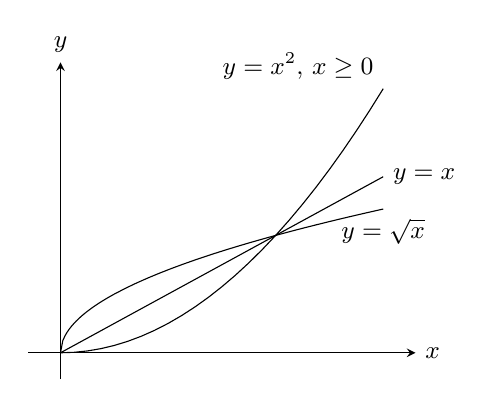
\begin{tikzpicture}[font=\small,declare function={f(\x)=\x^2;g(\x)=sqrt(\x);h(\x)=\x;}]
\begin{axis}[clip=false,small,axis lines=middle,enlargelimits=true,xlabel={$x$},ylabel={$y$},xlabel style={at={(current axis.right of origin)},anchor=west},ylabel style={at={(current axis.above origin)},anchor=south},xtick={\empty},ytick={\empty}]
\addplot[domain=0:1.5]{f(x)}node[above left]{$y=x^2,\, x\ge 0$};
\addplot[domain=0:0.25]{g(x)};
\addplot[domain=0.25:1.5]{g(x)}node[below]{$y=\sqrt{x}$};
\addplot[domain=0:1.5]{h(x)}node[right]{$y=x$};
\end{axis}
\end{tikzpicture}
\caption{
تفاعل \عددی{y=\sqrt{x}} اور \عددی{y=x^2,\, x\ge 0} ایک دوسرے کے الٹ ہیں (مثال \حوالہ{مثال_ماورائی_الٹ_تفاعل_کی_مثال})۔
}
\label{شکل_ماورائی_الٹ_تفاعل_تعریف}
\end{minipage}\hfill
\begin{minipage}{0.45\textwidth}
\centering
\begin{tikzpicture}[font=\small,declare function={f(\x)=1+3*(\x-1);g(\x)=\x;}]
\begin{axis}[clip=false,small,axis lines=middle,enlargelimits=true,xlabel={$x$},ylabel={$y$},xlabel style={at={(current axis.right of origin)},anchor=west},ylabel style={at={(current axis.above origin)},anchor=south},xtick={\empty},ytick={\empty}]
\addplot[domain=-0.25:2.25]{f(x)}node[above,align=left,xshift=3ex]{$y=\tfrac{1}{m}x-\tfrac{b}{m}$\\ ڈھلوان $\tfrac{1}{m}$};
\addplot[domain=0.25:3]({f(x)},x)node[pos=0.85,below,align=center,xshift=1ex]{$y=mx+b$\\ ڈھلوان m};
\addplot[domain=-0.5:5]{g(x)}node[right]{$y=x$};
\end{axis}
\end{tikzpicture}
\caption{
لکیر \عددی{y=x} میں منعکس غیر انتصابی لکیروں کے ڈھلوان ایک دوسرے کے بالعکس متناسب ہوتے ہیں۔
}
\label{شکل_ماورائی_عکس_میں_تفرق_تعلق}
\end{minipage}
\end{figure}


\جزوحصہء{قابل تفرق تفاعل کے الٹ کے تفرق}
تفاعل \عددی{f(x)=\tfrac{x}{2}+1}  اور اس کے الٹ \عددی{f^{-1}(x)=2x-2} (مثال \حوالہ{مثال_ماورائی_الٹ}) کے تفرق درج ذیل ہیں۔
\begin{align*}
\frac{\dif}{\dif x}f(x)&=\frac{\dif}{\dif x}\big(\frac{x}{2}+1\big)=\frac{1}{2}\\
\frac{\dif}{\dif x}f^{-1}(x)&=\frac{\dif}{\dif x}(2x-2)=2
\end{align*}
یہ تفرقات ایک دوسرے کے بالعکس متناسب ہیں۔ تفاعل \عددی{f} کی ترسیم لکیر \عددی{y=\tfrac{x}{2}+1} اور \عددی{f^{-1}} کی ترسیم لکیر \عددی{y=2x-2} ہے۔ ان لکیروں کے ڈھلوان ایک دوسرے کے بالعکس متناسب ہیں (شکل \حوالہ{شکل_ماورائی_عکس_میں_تفرق_تعلق})۔

یہ نتیجہ کسی مخصوص تفاعل کے لئے نہیں ہے۔ لکیر \عددی{y=x} میں کسی بھی غیر افقی یا غیر انتصابی لکیر کے عکس کا ڈھلوان اس لکیر کے ڈھلوان کے بالعکس متناسب ہو گا۔ یوں اگر دیے گئے لکیر کا ڈھلوان \عددی{m\ne 0} (شکل \حوالہ{شکل_ماورائی_عکس_میں_تفرق_تعلق}) ہو تب منعکس لکیر کا ڈھلوان \عددی{\tfrac{1}{m}} ہو گا۔ 

تفاعل اور اس کے الٹ کے ڈھلوانوں  کا بالعکس متناسب تعلق دیگر تفاعل کو بھی مطمئن کرتا ہے۔ اگر نقطہ \عددی{(a,f(a))} پر \عددی{y=f(x)} کا ڈھلوان \عددی{f'(a)\ne 0} ہو تب مطابقتی نقطہ \عددی{(f(a),a)} پر \عددی{y=f^{-1}(x)} کا ڈھلوان \عددی{\tfrac{1}{f'(a)}} ہو گا (شکل \حوالہ{شکل_ماورائی_ڈھلوان_بالعکس_متناسب})۔ یوں نقطہ \عددی{f(a)} پر \عددی{f^{-1}} کا تفرق، نقطہ \عددی{a} پر \عددی{f} کے تفرق کا بالعکس متناسب ہو گا۔ یہ تعلق اس صورت درست ہو گا جب \عددی{f} درج ذیل مسئلہ میں پیش   شرائط کو مطمئن کرتا ہو۔ یہ شرائط اعلٰی احصاء سے حاصل ہوتے ہیں۔ 

\begin{figure}
\centering
\begin{subfigure}{0.45\textwidth}
\centering
\begin{tikzpicture}[font=\small,declare function={f(\x)=(\x-1)^2;g(\x)=1+sqrt(\x);ta(\x)=9/16+3/2*(\x-7/4);}]
\pgfmathsetmacro{\a}{1.75}
\pgfmathsetmacro{\b}{f(\a)}
\begin{axis}[clip=false,small,axis lines=middle,enlargelimits=true,xlabel={$x$},ylabel={$y$},xlabel style={at={(current axis.right of origin)},anchor=west},ylabel style={at={(current axis.above origin)},anchor=south},xtick={\a}, xticklabels={$a$}, ytick={\b}, yticklabels={$f(a)$}]
\addplot[domain=1:2.2]{f(x)}node[above left]{$y=f(x)$};
%\addplot[domain=0:0.5]{g(x)};
%\addplot[domain=0.5:1.5]{g(x)};
\draw(\a,\b)node[circ]{}node[right,yshift=-1ex]{$(a,f(a))$};
%\draw(\b,\a)node[circ]{};
\addplot[domain=1.25:2.2]{ta(x)};
%\addplot[domain=1.25:2.25]({ta(x)},x);
\end{axis}
\end{tikzpicture}
\end{subfigure}\hfill
\begin{subfigure}{0.45\textwidth}
\centering
\begin{tikzpicture}[font=\small,declare function={f(\x)=(\x-1)^2;g(\x)=1+sqrt(\x);ta(\x)=9/16+3/2*(\x-7/4);}]
\pgfmathsetmacro{\a}{1.75}
\pgfmathsetmacro{\b}{f(\a)}
\begin{axis}[clip=false,small,axis lines=middle,enlargelimits=true,xlabel={$x$},ylabel={$y$},xlabel style={at={(current axis.right of origin)},anchor=west},ylabel style={at={(current axis.above origin)},anchor=south},xtick={\b},xticklabels={$f(a)$},ytick={\a},yticklabels={$a$}]
%\addplot[domain=1:2.2]{f(x)};
\addplot[domain=0:0.5]{g(x)};
\addplot[domain=0.5:1.5]{g(x)}node[pos=0.75,below right]{$y=f^{-1}(x)$};
%\draw(\a,\b)node[circ]{};
\draw(\b,\a)node[circ]{}node[right,yshift=-1ex]{$(f(a),a)$};
%\addplot[domain=1:2.2]{ta(x)};
\addplot[domain=1.4:2.25]({ta(x)},x);
\end{axis}
\end{tikzpicture}
\end{subfigure}
\caption{
الٹ تفاعل کے مطابقتی نقطوں پر ڈھلوان ایک دوسرے کا بالعکس متناسب 
\عددی{\left.\tfrac{\dif f^{-1}}{\dif x}\right\vert_{f(a)}=\tfrac{1}{\left.\tfrac{\dif f}{\dif x}\right\vert_{a}}} ہو گا۔
}
\label{شکل_ماورائی_ڈھلوان_بالعکس_متناسب}
\end{figure}
\ابتدا{مسئلہ}\شناخت{مسئلہ_ماورائی_الٹ_تفرق_قاعدہ}\موٹا{الٹ تفاعل کے تفرق کا قاعدہ}\\
اگر وقفہ \عددی{I} کے ہر نقطہ پر \عددی{f} قابل تفرق ہو اور \عددی{I} پر \عددی{\tfrac{\dif f}{\dif x}} کبھی بھی صفر  نہ ہو، تب وقفہ \عددی{f(I)} کے ہر نقطہ پر \عددی{f^{-1}} قابل تفرق ہو گا۔ کسی ایک مخصوص نقطہ \عددی{f(a)} پر \عددی{\tfrac{\dif f^{-1}}{\dif x}} کا تفرق نقطہ \عددی{a} پر تفرق \عددی{\tfrac{\dif f}{\dif x}} کا بالعکس متناسب ہو گا:
\begin{align}\label{مساوات_ماورائی_قاعدہ_الٹ_تفرق_الف}
\big(\frac{\dif f^{-1}}{\dif x}\big)_{x=f(a)}=\frac{1}{\big(\frac{\dif f}{\dif x}\big)_{x=a}}
\end{align}
اس کو مختصراً درج ذیل لکھا جا سکتا ہے۔
\begin{align}\label{مساوات_ماورائی_قاعدہ_الٹ_تفرق_ب}
(f^{-1})'=\frac{1}{f'}
\end{align}
\انتہا{مسئلہ}
%==================

\ابتدا{مثال}\شناخت{مثال_ماورائی_تفرق_الٹ_تفرق}
تفاعل \عددی{f(x)=x^2,\,x\ge 0} اور اس کے الٹ \عددی{f^{-1}(x)=\sqrt{x}} کے لئے درج ذیل لکھا جا سکتا ہے۔
\begin{align*}
\frac{\dif f}{\dif x}=\frac{\dif}{\dif x}(x^2)=2x,\quad \frac{\dif f^{-1}}{\dif x}=\frac{\dif}{\dif x}\sqrt{x}=\frac{1}{2\sqrt{x}},\,\,x>0
\end{align*}
نقطہ \عددی{(4,2)} لکیر \عددی{y=x} کی دوسری طرف نقطہ \عددی{(2,4)} کا عکس ہے (شکل \حوالہ{شکل_مثال_ماورائی_تفرق_الٹ_تفرق})۔ان نقطوں پر درج ذیل حاصل ہو گا۔
\begin{align*}
\frac{\dif f}{\dif x}&=2x=2(2)=4&&\text{\RL{نقطہ $(2,4)$ پر}}\\
\frac{\dif f^{-1}}{\dif x}&=\frac{1}{2\sqrt{x}}=\frac{1}{2\sqrt{4}}=\frac{1}{4}=\frac{1}{\dif f/\dif x}&&\text{\RL{نقطہ $(4,2)$ پر}}
\end{align*}
\انتہا{مثال}
%====================
\begin{figure}
\centering
\begin{minipage}{0.45\textwidth}
\centering
\begin{tikzpicture}[font=\small,declare function={f(\x)=\x^2;ta(\x)=4+4*(\x-2);tb(\x)=2+1/4*(\x-4);}]
\begin{axis}[clip=false,small,axis lines=middle,enlargelimits=true,xlabel={$x$},ylabel={$y$},xlabel style={at={(current axis.right of origin)},anchor=west},ylabel style={at={(current axis.above origin)},anchor=south},xtick={2,4},ytick={2,4}]
\addplot[domain=0:2.5]{f(x)}node[above,xshift=3ex]{$y=x^2,\, x \ge 0$};
\addplot[domain=0:3]({f(x)},{x})node[below]{$y=\tfrac{1}{\sqrt{x}}$};
\addplot[thick,domain=1.5:2.5]{ta(x)};
\addplot[thick,domain=2.5:8]{tb(x)};
\draw(2,4)node[circ]{}node[left]{$(2,4)$}node[right]{ڈھلوان 4};
\draw(4,2)node[circ]{}node[below]{$(4,2)$}node[above]{ڈھلوان $\tfrac{1}{4}$};
\end{axis}
\end{tikzpicture}
\caption{
نقطہ \عددی{(4,2)} پر \عددی{f^{-1}(x)=\sqrt{x}} کا تفرق نقطہ \عددی{(2,4)} پر \عددی{f(x)=x^2} کے تفرق کا بالعکس متناسب ہو گا (مثال \حوالہ{مثال_ماورائی_تفرق_الٹ_تفرق})۔
}
\label{شکل_مثال_ماورائی_تفرق_الٹ_تفرق}
\end{minipage}\hfill
\begin{minipage}{0.45\textwidth}
\centering
\begin{tikzpicture}[font=\small,declare function={f(\x)=\x^3-2;g(\x)=(\x+2)^(1/3); ta(\x)=6+12*(\x-2);tb(\x)=2+1/12*(\x-6);}]
\begin{axis}[clip=false,small,axis lines=middle,enlargelimits=true,xlabel={$x$},ylabel={$y$},xlabel style={at={(current axis.right of origin)},anchor=west},ylabel style={at={(current axis.above origin)},anchor=south},xtick={-2,6},ytick={-2,6}]
\addplot[domain=0:2.05]{f(x)}node[above,xshift=3ex]{$y=x^3-2$};
\addplot[domain=-2:-1.5]{g(x)};
\addplot[domain=-1.5:7]{g(x)};
\addplot[thick,domain=1.75:2.05]{ta(x)};
\addplot[thick,domain=3:7]{tb(x)};
\draw(2,6)node[circ]{}node[left]{$(2,6)$}node[right]{ڈھلوان 12};
\draw(6,2)node[circ]{}node[below]{$(6,2)$}node[above]{الٹ ڈھلوان $\tfrac{1}{12}$};
\end{axis}
\end{tikzpicture}
\caption{
نقطہ \عددی{x=2} پر \عددی{f(x)=x^3-2} کا تفرق ہمیں نقطہ \عددی{x=6} پر \عددی{f^{-1}} کا تفرق دیتا  ہے (مثال \حوالہ{مثال_ماورائی_ایک_نقطہ_پر_تفرق_سے_الٹ_تفرق_کا_حصول})۔
}
\label{شکل_مثال_ماورائی_ایک_نقطہ_پر_تفرق_سے_الٹ_تفرق_کا_حصول}
\end{minipage}
\end{figure}

بعض اوقات \عددی{f^{-1}} کا کلیہ نہ جانتے ہوئے بھی مساوات \حوالہ{مساوات_ماورائی_قاعدہ_الٹ_تفرق_الف} کی مدد سے \عددی{\tfrac{\dif f^{-1}}{\dif x}} کی مخصوص قیمتیں تلاش کی جا سکتی ہیں۔

\ابتدا{مثال}\شناخت{مثال_ماورائی_ایک_نقطہ_پر_تفرق_سے_الٹ_تفرق_کا_حصول}
مان لیں \عددی{f(x)=x^3-2} ہے۔ \عددی{f^{-1}(x)} کا کلیہ دریافت کیے بغیر نقطہ \عددی{x=6=f(2)} پر \عددی{\tfrac{\dif f^{-1}}{\dif x}} کی قیمت تلاش کریں۔

حل:  (شکل \حوالہ{شکل_مثال_ماورائی_ایک_نقطہ_پر_تفرق_سے_الٹ_تفرق_کا_حصول})
\begin{align*}
\left.\frac{\dif f}{\dif x}\right\vert_{x=2}&=\left.3x^2\right\vert_{x=2}=12\\
\left.\frac{\dif f^{-1}}{\dif x}\right\vert_{x=f(2)}&=\frac{1}{12}&&\text{\RL{مساوات \حوالہ{مساوات_ماورائی_قاعدہ_الٹ_تفرق_الف}}}
\end{align*}
\انتہا{مثال}
%=======================

مسئلہ \حوالہ{مسئلہ_ماورائی_الٹ_تفرق_قاعدہ} کو ایک مختلف نقطہ نظر سے دیکھا جا سکتا ہے۔ اگر \عددی{x=a} پر \عددی{y=f(x)}  قابل تفرق ہو اور ہم \عددی{x} کی قیمت میں معمولی تبدیلی \عددی{\dif x} لائیں تب \عددی{y} میں مطابقتی تبدیلی تخمیناً
\begin{align*}
\dif y=f'(a)\dif x
\end{align*}
ہو گا۔اس کا مطلب ہے کہ \عددی{y} کی تبدیلی، \عددی{x} کی تبدیلی کے تقریباً \عددی{f'(a)} گنّا ہو گی اور \عددی{x} کی تبدیلی، \عددی{y} کی تبدیلی کے تقریباً  \عددی{\tfrac{1}{f'(a)}} گنّا ہو گی۔

\حصہء{سوالات}
\موٹا{ایک ایک تفاعل کی نشاندہی}\\
سوال \حوالہ{سوال_ماورائی_ایک_ایک_نشاندہی_الف} تا سوال \حوالہ{سوال_ماورائی_ایک_ایک_نشاندہی_ث} میں تفاعل کے ترسیم دیے گئے ہیں۔ ان میں  ایک ایک تفاعل کی نشاندہی کریں۔

\ابتدا{سوال}\شناخت{سوال_ماورائی_ایک_ایک_نشاندہی_الف}
ترسیم شکل \حوالہ{شکل_سوال_ماورائی_ایک_ایک_نشاندہی_الف} میں دی گئی ہے۔\\
جواب:\quad
ایک ایک
\انتہا{سوال}
%=======================
\ابتدا{سوال}\شناخت{سوال_ماورائی_ایک_ایک_نشاندہی_ب}
ترسیم شکل \حوالہ{شکل_سوال_ماورائی_ایک_ایک_نشاندہی_ب} میں دی گئی ہے۔
\انتہا{سوال}
%=======================
\ابتدا{سوال}\شناخت{سوال_ماورائی_ایک_ایک_نشاندہی_پ}
ترسیم شکل \حوالہ{شکل_سوال_ماورائی_ایک_ایک_نشاندہی_پ} میں دی گئی ہے۔\\
جواب:\quad
غیر ایک ایک
\انتہا{سوال}
%=======================
\ابتدا{سوال}\شناخت{سوال_ماورائی_ایک_ایک_نشاندہی_ت}
ترسیم شکل \حوالہ{شکل_سوال_ماورائی_ایک_ایک_نشاندہی_ت} میں دی گئی ہے۔
\انتہا{سوال}
%=======================
\ابتدا{سوال}\شناخت{سوال_ماورائی_ایک_ایک_نشاندہی_ٹ}
ترسیم شکل \حوالہ{شکل_سوال_ماورائی_ایک_ایک_نشاندہی_ٹ} میں دی گئی ہے۔\\
جواب:\quad
ایک ایک
\انتہا{سوال}
%=======================
\ابتدا{سوال}\شناخت{سوال_ماورائی_ایک_ایک_نشاندہی_ث}
ترسیم شکل \حوالہ{شکل_سوال_ماورائی_ایک_ایک_نشاندہی_ث} میں دی گئی ہے۔
\انتہا{سوال}
%=================
\begin{figure}
\centering
\begin{minipage}{0.3\textwidth}
\centering
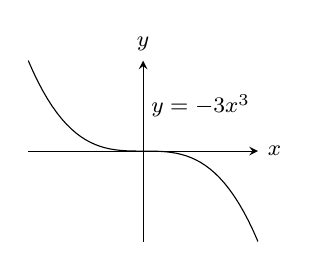
\begin{tikzpicture}[font=\footnotesize,declare function={f(\x)=-3*\x^3;}]
\begin{axis}[width=4.5cm,axis lines=middle,xlabel={$x$},ylabel={$y$},xlabel style={at={(current axis.right of origin)},anchor=west},ylabel style={at={(current axis.above origin)},anchor=south},xtick={\empty},ytick={\empty}]
\addplot[domain=0:2]{f(x)};
\addplot[domain=0:2]({-x},{-f(x)});
\draw(1,{-1/2*f(2)})node[]{$y=-3x^3$};
\end{axis}
\end{tikzpicture}
\caption{ترسیم سوال \حوالہ{سوال_ماورائی_ایک_ایک_نشاندہی_الف}}
\label{شکل_سوال_ماورائی_ایک_ایک_نشاندہی_الف}
\end{minipage}\hfill
\begin{minipage}{0.3\textwidth}
\centering
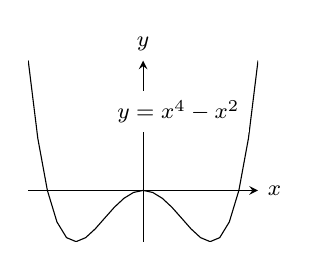
\begin{tikzpicture}[font=\footnotesize,declare function={f(\x)=\x^4-\x^2;}]
\begin{axis}[width=4.5cm,axis lines=middle,xlabel={$x$},ylabel={$y$},xlabel style={at={(current axis.right of origin)},anchor=west},ylabel style={at={(current axis.above origin)},anchor=south},xtick={\empty},ytick={\empty}]
\addplot[domain=-1.2:1.2]{f(x)}node[pos=0.9,above left,fill=white]{$y=x^4-x^2$};
\end{axis}
\end{tikzpicture}
\caption{ترسیم سوال \حوالہ{سوال_ماورائی_ایک_ایک_نشاندہی_ب}}
\label{شکل_سوال_ماورائی_ایک_ایک_نشاندہی_ب}
\end{minipage}\hfill
\begin{minipage}{0.3\textwidth}
\centering
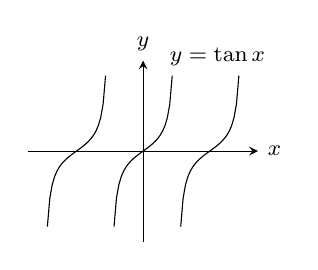
\begin{tikzpicture}[font=\footnotesize,declare function={f(\x)=tan(deg(\x));}]
\begin{axis}[clip=false,width=4.5cm,axis lines=middle,xlabel={$x$},ylabel={$y$},xlabel style={at={(current axis.right of origin)},anchor=west},ylabel style={at={(current axis.above origin)},anchor=south},xtick={\empty},ytick={\empty},enlargelimits=true]
\addplot[domain=-3/2*pi+0.2:-pi/2-0.2]{f(x)};
\addplot[domain=-pi/2+0.2:pi/2-0.2]{f(x)};
\addplot[domain=pi/2+0.2:3/2*pi-0.2]{f(x)}node[above  left,xshift=3ex]{$y=\tan x$};
\end{axis}
\end{tikzpicture}
\caption{ترسیم سوال \حوالہ{سوال_ماورائی_ایک_ایک_نشاندہی_پ}}
\label{شکل_سوال_ماورائی_ایک_ایک_نشاندہی_پ}
\end{minipage}
\end{figure}
%======================
\begin{figure}
\centering
\begin{minipage}{0.3\textwidth}
\centering
\begin{tikzpicture}[font=\footnotesize,declare function={f(\x)=-3*\x^3;}]
\pgfmathsetmacro{\k}{1.25/5}
\draw[-latex](-1.25,0)--(1.25,0)node[right]{$x$};
\draw[-latex](0,-1.25)--(0,1.25)node[above]{$y$};
\foreach \x in {-1,-2,-3,-4,0,1,2,3}{\draw(\x*\k,\x*\k)node[circ]{}--++(\k,0)node[ocirc]{};}
\draw(-0.75,0.75)node[]{$y=\lfloor x\rfloor$};
\end{tikzpicture}
\caption{ترسیم سوال \حوالہ{سوال_ماورائی_ایک_ایک_نشاندہی_ت}}
\label{شکل_سوال_ماورائی_ایک_ایک_نشاندہی_ت}
\end{minipage}\hfill
\begin{minipage}{0.3\textwidth}
\centering
\begin{tikzpicture}[font=\footnotesize,declare function={f(\x)=1/\x;}]
\begin{axis}[width=4.5cm,axis lines=middle,xlabel={$x$},ylabel={$y$},xlabel style={at={(current axis.right of origin)},anchor=west},ylabel style={at={(current axis.above origin)},anchor=south},xtick={\empty},ytick={\empty}]
\addplot[domain=0.2:5]{f(x)}node[pos=0.25,right]{$y=\tfrac{1}{x}$};
\addplot[domain=0.2:5](-x,{-f(x)});
\end{axis}
\end{tikzpicture}
\caption{ترسیم سوال \حوالہ{سوال_ماورائی_ایک_ایک_نشاندہی_ٹ}}
\label{شکل_سوال_ماورائی_ایک_ایک_نشاندہی_ٹ}
\end{minipage}\hfill
\begin{minipage}{0.3\textwidth}
\centering
\begin{tikzpicture}[font=\footnotesize,declare function={f(\x)=\x^(1/3);}]
\begin{axis}[clip=false,width=4.5cm,axis lines=middle,xlabel={$x$},ylabel={$y$},xlabel style={at={(current axis.right of origin)},anchor=west},ylabel style={at={(current axis.above origin)},anchor=south},xtick={\empty},ytick={\empty},enlargelimits=true]
\addplot[domain=0:6]{f(x)};
\draw (-3,1)node[]{$y=x^{1/3}$};
\addplot[domain=0:6](-x,{-f(x)});
\end{axis}
\end{tikzpicture}
\caption{ترسیم سوال \حوالہ{سوال_ماورائی_ایک_ایک_نشاندہی_ث}}
\label{شکل_سوال_ماورائی_ایک_ایک_نشاندہی_ث}
\end{minipage}
\end{figure}

\موٹا{الٹ تفاعل کی ترسیم}\\
سوال \حوالہ{سوال_ماورائی_ترسیم_دیا_الف} تا سوال \حوالہ{سوال_ماورائی_ترسیم_دیا_ت} میں \عددی{y=f(x)} کی ترسیم دی گئی ہے۔ اس کو نقل کر کے لکیر  \عددی{y=x} بھی بنائیں۔ لکیر \عددی{y=x} کے لحاظ سے تشاکلی استعمال کرتے ہوئے \عددی{y=f^{-1}(x)} ترسیم کریں۔(\عددی{f^{-1}} کا کلیہ معلوم کرنے کی ضرورت نہیں ہے۔) \عددی{f^{-1}} کے دائرہ کار اور سعت کی نشاندہی  کریں۔

\ابتدا{سوال}\شناخت{سوال_ماورائی_ترسیم_دیا_الف}
تفاعل کی ترسیم شکل \حوالہ{شکل_سوال_ماورائی_ترسیم_دیا_الف} میں دی گئی ہے۔\\
جواب:\quad
دائرہ کار \عددی{(0,1]}، سعت \عددی{[0,\infty)}، شکل \حوالہ{شکل_جواب_ماورائی_ترسیم_دیا_الف}
\انتہا{سوال}
%=======================
\ابتدا{سوال}\شناخت{سوال_ماورائی_ترسیم_دیا_ب}
تفاعل کی ترسیم شکل \حوالہ{شکل_سوال_ماورائی_ترسیم_دیا_ب} میں دی گئی ہے۔
\انتہا{سوال}
%=======================
\ابتدا{سوال}\شناخت{سوال_ماورائی_ترسیم_دیا_پ}
تفاعل کی ترسیم شکل \حوالہ{شکل_سوال_ماورائی_ترسیم_دیا_پ} میں دی گئی ہے۔\\
جواب:\quad
دائرہ کار \عددی{[-1,1]}، سعت \عددی{-\tfrac{\pi}{2},\tfrac{\pi}{2}} ،شکل \حوالہ{شکل_جواب_ماورائی_ترسیم_دیا_پ}
\انتہا{سوال}
%=======================
\ابتدا{سوال}\شناخت{سوال_ماورائی_ترسیم_دیا_ت}
تفاعل کی ترسیم شکل \حوالہ{شکل_سوال_ماورائی_ترسیم_دیا_ت} میں دی گئی ہے۔
\انتہا{سوال}
%=======================
\begin{figure}
\centering
\begin{minipage}{0.2\textwidth}
\centering
\begin{tikzpicture}[font=\tiny,declare function={f(\x)=1/(\x^2+1);}]
\begin{axis}[clip=false,width=4cm,axis lines=middle,xlabel={$x$},ylabel={$y$},xlabel style={at={(current axis.right of origin)},anchor=west},ylabel style={at={(current axis.above origin)},anchor=south},xtick={1},ytick={1},enlargelimits=true,ymin=0]
\addplot[domain=0:2]{f(x)}node[pos=0.5,above right]{$\begin{aligned}y&=f(x)\\ &=\frac{1}{\x^2+1},\, x\ge 0\end{aligned}$};
\end{axis}
\end{tikzpicture}
\caption{ترسیم سوال \حوالہ{سوال_ماورائی_ترسیم_دیا_الف}}
\label{شکل_سوال_ماورائی_ترسیم_دیا_الف}
\end{minipage}\hfill
\begin{minipage}{0.2\textwidth}
\centering
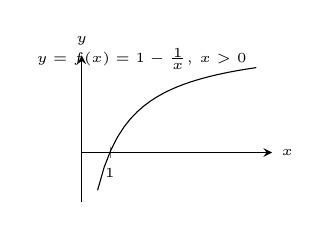
\begin{tikzpicture}[font=\tiny,declare function={f(\x)=1-1/\x;}]
\begin{axis}[clip=false,width=4cm,axis lines=middle,xlabel={$x$},ylabel={$y$},xlabel style={at={(current axis.right of origin)},anchor=west},ylabel style={at={(current axis.above origin)},anchor=south},xtick={1},ytick={1},enlargelimits=true]
\addplot[domain=0.75:4]{f(x)}node[pos=1,above left,yshift=-1ex]{$y=f(x)=1-\frac{1}{x},\, x> 0$};
\end{axis}
\end{tikzpicture}
\caption{ترسیم سوال \حوالہ{سوال_ماورائی_ترسیم_دیا_ب}}
\label{شکل_سوال_ماورائی_ترسیم_دیا_ب}
\end{minipage}\hfill
\begin{minipage}{0.2\textwidth}
\centering
\begin{tikzpicture}[font=\tiny,declare function={f(\x)=sin(deg(\x));}]
\pgfmathsetmacro{\k}{1/2*pi}
\begin{axis}[clip=false,width=4cm,axis lines=middle,xlabel={$x$},ylabel={$y$},xlabel style={at={(current axis.right of origin)},anchor=west},ylabel style={at={(current axis.above origin)},anchor=south},xtick={-\k,\k},xticklabels={$-\tfrac{\pi}{2}$,$\tfrac{\pi}{2}$},ytick={-1,1},enlargelimits=true]
\addplot[domain=-1/2*pi:1/2*pi]{f(x)};
\draw(-1/2*pi,1)node[]{$\begin{aligned}y&=f(x)=\sin x\\  &-\tfrac{\pi}{2}\le x\le \tfrac{\pi}{2}\end{aligned}$};
\draw(-\k,-1)node[circ]{}  (\k,1)node[circ]{};
\end{axis}
\end{tikzpicture}
\caption{ترسیم سوال \حوالہ{سوال_ماورائی_ترسیم_دیا_پ}}
\label{شکل_سوال_ماورائی_ترسیم_دیا_پ}
\end{minipage}\hfill
\begin{minipage}{0.2\textwidth}
\centering
\begin{tikzpicture}[font=\tiny,declare function={f(\x)=tan(deg(\x));}]
\pgfmathsetmacro{\k}{1/2*pi}
\begin{axis}[clip=false,width=4cm,axis lines=middle,xlabel={$x$},ylabel={$y$},xlabel style={at={(current axis.right of origin)},anchor=west},ylabel style={at={(current axis.above origin)},anchor=south}, xtick={-\k,\k},  xticklabels={$-\tfrac{\pi}{2}$,$\tfrac{\pi}{2}$}, ytick={\empty},xmin=-\k-0.1,xmax=\k+0.2]
\addplot[domain=-\k+0.4:\k-0.4]{f(x)};
\draw(-1/2*pi,2)node[]{$\begin{aligned}y&=f(x)=\tan x\\  &-\tfrac{\pi}{2}< x<\tfrac{\pi}{2}\end{aligned}$};
\end{axis}
\end{tikzpicture}
\caption{ترسیم سوال \حوالہ{سوال_ماورائی_ترسیم_دیا_ت}}
\label{شکل_سوال_ماورائی_ترسیم_دیا_ت}
\end{minipage}
\end{figure}
%
\begin{figure}
\centering
\begin{minipage}{0.3\textwidth}
\centering
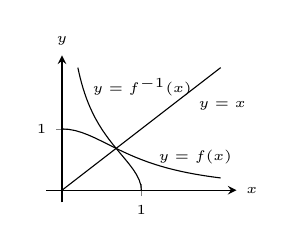
\begin{tikzpicture}[font=\tiny,declare function={f(\x)=1/(\x^2+1);m(\x)=\x;}]
\begin{axis}[clip=false,width=4cm,axis lines=middle,xlabel={$x$},ylabel={$y$},xlabel style={at={(current axis.right of origin)},anchor=west},ylabel style={at={(current axis.above origin)},anchor=south},xtick={1},ytick={1},enlargelimits=true,ymin=0]
\addplot[domain=0:2]{f(x)}node[pos=0.85,above]{$y=f(x)$};
\addplot[domain=0:2]({f(x)},x)node[pos=0.85,right]{$y=f^{-1}(x)$};
\addplot[domain=0:2]{m(x)}node[pos=0.8,below right]{$y=x$};
\end{axis}
\end{tikzpicture}
\caption{ترسیم جواب \حوالہ{سوال_ماورائی_ترسیم_دیا_الف}}
\label{شکل_جواب_ماورائی_ترسیم_دیا_الف}
\end{minipage}\hfill
\begin{minipage}{0.3\textwidth}
\centering
\begin{tikzpicture}[font=\tiny,declare function={f(\x)=sin(deg(\x));m(\x)=\x;}]
\pgfmathsetmacro{\k}{1/2*pi}
\begin{axis}[clip=false,width=4cm,axis lines=middle,xlabel={$x$},ylabel={$y$},xlabel style={at={(current axis.right of origin)},anchor=west},ylabel style={at={(current axis.above origin)},anchor=south},xtick={-\k,\k},xticklabels={$-\tfrac{\pi}{2}$,$\tfrac{\pi}{2}$},ytick={-1,1},enlargelimits=true]
\addplot[domain=-1/2*pi:1/2*pi]{f(x)}node[right]{$y=f(x)$};
\addplot[domain=-1/2*pi:1/2*pi]({f(x)},x)node[above]{$y=f^{-1}(x)$};
\addplot[domain=-1/2*pi:1/2*pi]{m(x)}node[right]{$y=x$};
%\draw(-1/2*pi,1)node[]{$\begin{aligned}y&=f(x)=\sin x\\  &-\tfrac{\pi}{2}\le x\le \tfrac{\pi}{2}\end{aligned}$};
\end{axis}
\end{tikzpicture}
\caption{ترسیم جواب \حوالہ{سوال_ماورائی_ترسیم_دیا_پ}}
\label{شکل_جواب_ماورائی_ترسیم_دیا_پ}
\end{minipage}\hfill
\begin{minipage}{0.3\textwidth}
\centering
\begin{tikzpicture}[font=\tiny,declare function={f(\x)=sqrt(1-\x^2);m(\x)=\x;}]
\pgfmathsetmacro{\k}{1/2*pi}
\begin{axis}[clip=false,width=4cm,axis lines=middle,xlabel={$x$},ylabel={$y$},xlabel style={at={(current axis.right of origin)},anchor=west},ylabel style={at={(current axis.above origin)},anchor=south},xtick={1},ytick={1},enlargelimits=true]
\addplot[domain=0:0.9]{f(x)}node[pos=0.5,above right]{$\begin{aligned}y&=f(x)\\  0&\le x\le 1\end{aligned}$};
\addplot[domain=0.9:1]{f(x)};
\end{axis}
\end{tikzpicture}
\caption{ترسیم جواب \حوالہ{سوال_ماورائی_تشاکلی_دریافت_الف}}
\label{شکل_جواب_ماورائی_تشاکلی_دریافت_الف}
\end{minipage}
\end{figure}

\ابتدا{سوال}\شناخت{سوال_ماورائی_تشاکلی_دریافت_الف}
(ا) تفاعل \عددی{f(x)=\sqrt{1-x^2},\, 0\le x\le 1} ترسیم کریں۔ اس ترسیم میں کون سی تشاکلی پائی جاتی ہے؟ (ب) دکھائیں کہ \عددی{f} اپنا ہی الٹ ہے۔ (یاد رہے کہ \عددی{x\ge 0} کی صورت میں \عددی{\sqrt{x^2}=x} ہوتا ہے۔)\\
جواب:\quad
لکیر \عددی{y=x} کے لحاظ سے تشاکلی ہے۔ شکل \حوالہ{شکل_جواب_ماورائی_تشاکلی_دریافت_الف}
\انتہا{سوال}
%==============
\ابتدا{سوال}
(ا) تفاعل \عددی{f(x)=\tfrac{1}{x}} ترسیم کریں۔ اس ترسیم میں کون سی تشاکلی پائی جاتی ہے؟ (ب) دکھائیں کہ \عددی{f} اپنا ہی الٹ ہے۔
\انتہا{سوال}
%==================
\موٹا{الٹ تفاعل کے کلیات}\\
سوال \حوالہ{سوال_ماورائی_ترسیم_کلیہ_الف} تا سوال \حوالہ{سوال_ماورائی_ترسیم_کلیہ_ث} میں تفاعل \عددی{y=f(x)} کا کلیہ دیا گیا ہے۔ \عددی{f} اور \عددی{f^{-1}} کی ترسیمات بھی دکھائی گئی ہیں۔ \عددی{f^{-1}} کا کلیہ تلاش کریں۔

\ابتدا{سوال}\شناخت{سوال_ماورائی_ترسیم_کلیہ_الف}
$f(x)=x^2+1,\quad x\ge 0$
ترسیم شکل \حوالہ{شکل_سوال_ماورائی_ترسیم_کلیہ_الف} میں دی گئی ہے۔\\
جواب:\quad
$f^{-1}(x)=\sqrt{x-1}$
\انتہا{سوال}
%===================
\ابتدا{سوال}\شناخت{سوال_ماورائی_ترسیم_کلیہ_ب}
$f(x)=x^2,\quad x\le 0$
ترسیم شکل \حوالہ{شکل_سوال_ماورائی_ترسیم_کلیہ_ب} میں دی گئی ہے۔
\انتہا{سوال}
%===================
\ابتدا{سوال}\شناخت{سوال_ماورائی_ترسیم_کلیہ_پ}
$f(x)=x^3-1$
ترسیم شکل \حوالہ{شکل_سوال_ماورائی_ترسیم_کلیہ_پ} میں دی گئی ہے۔\\
جواب:\quad
$f^{-1}(x)=\sqrt[3]{x+1}$
\انتہا{سوال}
%===================
\ابتدا{سوال}\شناخت{سوال_ماورائی_ترسیم_کلیہ_ت}
$f(x)=x^2-2x+1,\quad x\ge 1$
ترسیم شکل \حوالہ{شکل_سوال_ماورائی_ترسیم_کلیہ_ت} میں دی گئی ہے۔
\انتہا{سوال}
%===================
\ابتدا{سوال}\شناخت{سوال_ماورائی_ترسیم_کلیہ_ٹ}
$f(x)=(x+1)^2,\quad x\ge -1$
ترسیم شکل \حوالہ{شکل_سوال_ماورائی_ترسیم_کلیہ_ٹ} میں دی گئی ہے۔\\
جواب:\quad
$f^{-1}(x)=\sqrt{x}-1$
\انتہا{سوال}
%===================
\ابتدا{سوال}\شناخت{سوال_ماورائی_ترسیم_کلیہ_ث}
$f(x)=x^{2/3},\quad x\ge 0$
ترسیم شکل \حوالہ{شکل_سوال_ماورائی_ترسیم_کلیہ_ث} میں دی گئی ہے۔
\انتہا{سوال}
%===================
\begin{figure}
\centering
\begin{minipage}{0.3\textwidth}
\centering
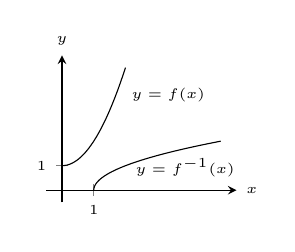
\begin{tikzpicture}[font=\tiny,declare function={f(\x)=\x^2+1;}]
\begin{axis}[clip=false,width=4cm,axis lines=middle,xlabel={$x$},ylabel={$y$},xlabel style={at={(current axis.right of origin)},anchor=west},ylabel style={at={(current axis.above origin)},anchor=south},xtick={1},ytick={1},enlargelimits=true,ymin=0]
\addplot[domain=0:2]{f(x)}node[pos=0.9,below right]{$y=f(x)$};
\addplot[domain=0:2]({f(x)},x)node[pos=0.75,below]{$y=f^{-1}(x)$};
\end{axis}
\end{tikzpicture}
\caption{ترسیم سوال \حوالہ{سوال_ماورائی_ترسیم_کلیہ_الف}}
\label{شکل_سوال_ماورائی_ترسیم_کلیہ_الف}
\end{minipage}\hfill
\begin{minipage}{0.3\textwidth}
\centering
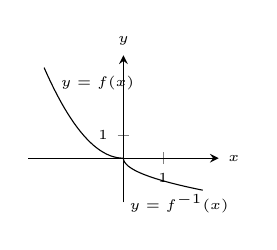
\begin{tikzpicture}[font=\tiny,declare function={f(\x)=\x^2;}]
\begin{axis}[clip=false,width=4cm,axis lines=middle,xlabel={$x$},ylabel={$y$},xlabel style={at={(current axis.right of origin)},anchor=west},ylabel style={at={(current axis.above origin)},anchor=south},xtick={1},ytick={1},enlargelimits=true]
\addplot[domain=0:2](-x,{f(x)})node[pos=0.85,right]{$y=f(x)$};
\addplot[domain=0:1.4142]({f(x)},-x)node[pos=0.75,below]{$y=f^{-1}(x)$};
\end{axis}
\end{tikzpicture}
\caption{ترسیم سوال \حوالہ{سوال_ماورائی_ترسیم_کلیہ_ب}}
\label{شکل_سوال_ماورائی_ترسیم_کلیہ_ب}
\end{minipage}\hfill
\begin{minipage}{0.3\textwidth}
\centering
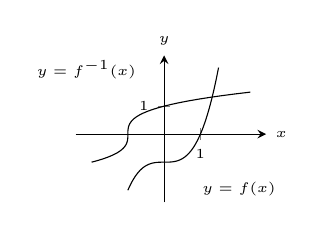
\begin{tikzpicture}[font=\tiny,declare function={f(\x)=\x^3-1;g(\x)=\x^3+1;}]
\begin{axis}[clip=false,width=4cm,axis lines=middle,xlabel={$x$},ylabel={$y$},xlabel style={at={(current axis.right of origin)},anchor=west},ylabel style={at={(current axis.above origin)},anchor=south},xtick={1},ytick={1},enlargelimits=true]
\addplot[domain=0:1.5]{f(x)}node[pos=0.25,below right,yshift={-2ex}]{$y=f(x)$};
\addplot[domain=0:1](-x,{-g(x)});
\addplot[domain=0:1.5]({f(x)},x)node[pos=0.25,above left,yshift=2ex]{$y=f^{-1}(x)$};
\addplot[domain=0:1]({-g(x)},-x);
\end{axis}
\end{tikzpicture}
\caption{ترسیم سوال \حوالہ{سوال_ماورائی_ترسیم_کلیہ_پ}}
\label{شکل_سوال_ماورائی_ترسیم_کلیہ_پ}
\end{minipage}
\end{figure}
%==============================
\begin{figure}
\centering
\begin{minipage}{0.3\textwidth}
\centering
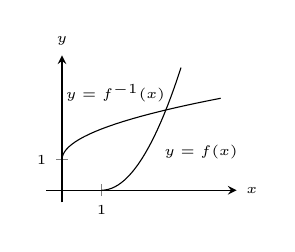
\begin{tikzpicture}[font=\tiny,declare function={f(\x)=\x^2-2*\x+1;}]
\begin{axis}[clip=false,width=4cm,axis lines=middle,xlabel={$x$},ylabel={$y$},xlabel style={at={(current axis.right of origin)},anchor=west},ylabel style={at={(current axis.above origin)},anchor=south},xtick={1},ytick={1},enlargelimits=true,ymin=0]
\addplot[domain=1:3]{f(x)}node[pos=0.5,below right]{$y=f(x)$};
\addplot[domain=1:3]({f(x)},x)node[pos=0.4,above,yshift=1ex]{$y=f^{-1}(x)$};
\end{axis}
\end{tikzpicture}
\caption{ترسیم سوال \حوالہ{سوال_ماورائی_ترسیم_کلیہ_ت}}
\label{شکل_سوال_ماورائی_ترسیم_کلیہ_ت}
\end{minipage}\hfill
\begin{minipage}{0.3\textwidth}
\centering
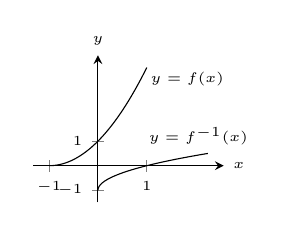
\begin{tikzpicture}[font=\tiny,declare function={f(\x)=(\x+1)^2;g(\x)=(\x-1)^2;}]
\begin{axis}[clip=false,width=4cm,axis lines=middle,xlabel={$x$},ylabel={$y$},xlabel style={at={(current axis.right of origin)},anchor=west},ylabel style={at={(current axis.above origin)},anchor=south},xtick={-1,1},ytick={-1,1},enlargelimits=true]
\addplot[domain=0:1](x,{f(x)})node[pos=0.85,right]{$y=f(x)$};
\addplot[domain=0:1](-x,{g(x)});
\addplot[domain=0:0.5]({f(x)},x)node[pos=0.85,above]{$y=f^{-1}(x)$};
\addplot[domain=0:1]({g(x)},-x);
\end{axis}
\end{tikzpicture}
\caption{ترسیم سوال \حوالہ{سوال_ماورائی_ترسیم_کلیہ_ٹ}}
\label{شکل_سوال_ماورائی_ترسیم_کلیہ_ٹ}
\end{minipage}\hfill
\begin{minipage}{0.3\textwidth}
\centering
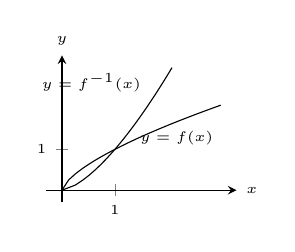
\begin{tikzpicture}[font=\tiny,declare function={f(\x)=(\x^2)^(1/3);}]
\begin{axis}[clip=false,width=4cm,axis lines=middle,xlabel={$x$},ylabel={$y$},xlabel style={at={(current axis.right of origin)},anchor=west},ylabel style={at={(current axis.above origin)},anchor=south},xtick={1},ytick={1},enlargelimits=true]
\addplot[domain=0:3]{f(x)}node[pos=0.75,below]{$y=f(x)$};
\addplot[domain=0:3]({f(x)},x)node[pos=0.75,above left,]{$y=f^{-1}(x)$};
\end{axis}
\end{tikzpicture}
\caption{ترسیم سوال \حوالہ{سوال_ماورائی_ترسیم_کلیہ_ث}}
\label{شکل_سوال_ماورائی_ترسیم_کلیہ_ث}
\end{minipage}
\end{figure}

سوال \حوالہ{سوال_ماورائی_تصدیق_الف} تا سوال \حوالہ{سوال_ماورائی_تصدیق_ب} میں تفاعل \عددی{y=f(x)} کا کلیہ دیا گیا ہے۔ \عددی{f^{-1}} دریافت کریں اور اس کے دائرہ کار اور سعت کی نشاندہی کریں۔ تصدیق کی خاطر دکھائیں کہ \عددی{f(f^{-1}(x))=f^{-1}(f(x))=x} ہے۔ 

\ابتدا{سوال}\شناخت{سوال_ماورائی_تصدیق_الف}
$f(x)=x^5$\\
جواب:\quad
$f^{-1}(x)=\sqrt[5]{x}$
 دائرہ کار \عددی{-\infty<x<\infty}، سعت \عددی{-\infty<y<\infty}
\انتہا{سوال}
%======================
\ابتدا{سوال}
$f(x)=x^4,\quad x\ge 0$
\انتہا{سوال}
%======================
\ابتدا{سوال}
$f(x)=x^3+1$\\
جواب:\quad
$f^{-1}(x)=\sqrt[3]{x-1}$
دائرہ کار \عددی{-\infty<x<\infty}، سعت \عددی{-\infty<y<\infty}
\انتہا{سوال}
%======================
\ابتدا{سوال}
$f(x)=\tfrac{x}{2}-\tfrac{7}{2}$
\انتہا{سوال}
%======================
\ابتدا{سوال}
$f(x)=\tfrac{1}{x^2},\quad x>0$\\
جواب:\quad
$f^{-1}(x)=\tfrac{1}{\sqrt{x}}$
دائرہ کار \عددی{x>0}، سعت \عددی{y>0}
\انتہا{سوال}
%======================
\ابتدا{سوال}\شناخت{سوال_ماورائی_تصدیق_ب}
$f(x)=\tfrac{1}{x^3},\quad x\ne 0$
\انتہا{سوال}
%======================
\موٹا{الٹ تفاعل کے تفرق}\\
سوال \حوالہ{سوال_ماورائی_تصدیق_تفرق_الف} تا سوال \حوالہ{سوال_ماورائی_تصدیق_تفرق_ب} میں درج ذیل اقدام کریں۔
\begin{enumerate}[a.]
\item
\عددی{f^{-1}(x)} تلاش کریں۔
\item
\عددی{f} اور \عددی{f^{-1}} کو ایک ساتھ ترسیم کریں۔
\item
نقطہ \عددی{x=a} پر \عددی{\tfrac{\dif f}{\dif x}} اور نقطہ \عددی{x=f(a)} پر \عددی{\tfrac{\dif f^{-1}}{\dif x}} کی قیمت حاصل کریں۔ تصدیق کریں کہ ان نقطوں پر \عددی{\tfrac{\dif f^{-1}}{\dif x}=\tfrac{1}{\big(\tfrac{\dif f}{\dif x}\big)}} ہو گا۔
\end{enumerate}

\ابتدا{سوال}\شناخت{سوال_ماورائی_تصدیق_تفرق_الف}
$f(x)=2x+3,\quad a=-1$\\
جواب:\quad
(ا) \عددی{f^{-1}(x)=\tfrac{x}{2}-\tfrac{3}{2}}، (ب) شکل \حوالہ{شکل_جواب_ماورائی_تصدیق_تفرق_الف}، (ج) \عددی{2,\tfrac{1}{2}}
\انتہا{سوال}
%============================
\ابتدا{سوال}
$f(x)=\tfrac{x}{5}+7,\quad a=-1$
\انتہا{سوال}
%============================
\ابتدا{سوال}\شناخت{سوال_ماورائی_تصدیق_تفرق_درکار_پ}
$f(x)=5-4x,\quad a=\tfrac{1}{2}$\\
جواب:\quad
(ا) \عددی{f^{-1}(x)=-\tfrac{x}{4}+\tfrac{5}{4}}، (ب) شکل \حوالہ{شکل_جواب_ماورائی_تصدیق_تفرق_درکار_پ}،  (ج) \عددی{-4,-\tfrac{1}{4}}
\انتہا{سوال}
%============================
\ابتدا{سوال}\شناخت{سوال_ماورائی_تصدیق_تفرق_ب}
$f(x)=2x^2,\quad x\ge 0,\quad a=5$
\انتہا{سوال}
%============================
\begin{figure}
\centering
\begin{minipage}{0.3\textwidth}
\centering
\begin{tikzpicture}[font=\tiny,declare function={f(\x)=2*\x+3;}]
\begin{axis}[clip=false,width=4cm,axis lines=middle,xlabel={$x$},ylabel={$y$},xlabel style={at={(current axis.right of origin)},anchor=west},ylabel style={at={(current axis.above origin)},anchor=south}, xtick={-1.5,3},xticklabels={$-\tfrac{3}{2}$,$3$},ytick={-1.5,3},yticklabels={$-\tfrac{3}{2}$,$3$}, enlargelimits=true]
\addplot[domain=-1.7:0.5]{f(x)}node[right]{$y=f(x)=2x+3$};
\addplot[domain=-1.7:0.5]({f(x)},x)node[above,]{$y=f^{-1}(x)=\tfrac{x}{2}-\tfrac{3}{2}$};
\end{axis}
\end{tikzpicture}
\caption{ترسیم جواب \حوالہ{سوال_ماورائی_تصدیق_تفرق_الف}}
\label{شکل_جواب_ماورائی_تصدیق_تفرق_الف}
\end{minipage}\hfill
\begin{minipage}{0.3\textwidth}
\centering
\begin{tikzpicture}[font=\tiny,declare function={f(\x)=-4*\x+5;}]
\begin{axis}[clip=false,width=4cm,axis lines=middle,xlabel={$x$},ylabel={$y$},xlabel style={at={(current axis.right of origin)},anchor=west},ylabel style={at={(current axis.above origin)},anchor=south}, xtick={1.25,5},xticklabels={$\tfrac{5}{4}$,$5$},ytick={1.25,5},yticklabels={$\tfrac{5}{4}$,$5$}, enlargelimits=true]
\addplot[domain=-0.5:1.5]{f(x)}node[pos=0.25,right]{$y=f(x)=-4x+5$};
\addplot[domain=-0.25:1.5]({f(x)},x)node[pos=0.5,above right]{$y=f^{-1}(x)=-\tfrac{x}{4}+\tfrac{5}{4}$};
\end{axis}
\end{tikzpicture}
\caption{ترسیم جواب \حوالہ{سوال_ماورائی_تصدیق_تفرق_درکار_پ}}
\label{شکل_جواب_ماورائی_تصدیق_تفرق_درکار_پ}
\end{minipage}\hfill
\begin{minipage}{0.3\textwidth}
\centering
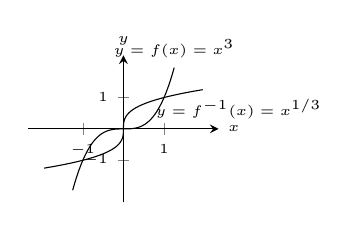
\begin{tikzpicture}[font=\tiny,declare function={f(\x)=\x^3;}]
\begin{axis}[clip=false,width=4cm,axis lines=middle,xlabel={$x$},ylabel={$y$},xlabel style={at={(current axis.right of origin)},anchor=west},ylabel style={at={(current axis.above origin)},anchor=south}, xtick={-1,1},ytick={-1,1}, enlargelimits=true]
\addplot[domain=0:1.25]{f(x)}node[above]{$y=f(x)=x^3$};
\addplot[domain=0:1.25](-x,{-f(x)});
\addplot[domain=0:1.25]({f(x)},x)node[below,xshift=3ex]{$y=f^{-1}(x)=x^{1/3}$};
\addplot[domain=0:1.25]({-f(x)},-x);
\end{axis}
\end{tikzpicture}
\caption{ترسیم جواب \حوالہ{سوال_ماورائی_تصدیق_تفرق_درکار_ت}}
\label{شکل_جواب_ماورائی_تصدیق_تفرق_درکار_ت}
\end{minipage}
\end{figure}
%===================================
\ابتدا{سوال}\شناخت{سوال_ماورائی_تصدیق_تفرق_درکار_ت}
\begin{enumerate}
\item
دکھائیں کہ \عددی{f(x)=x^3} اور \عددی{g(x)=\sqrt[3]{x}} ایک دوسرے کے الٹ ہیں۔
\item
\عددی{f} اور \عددی{g} ترسیم کریں جس میں ان کے نقاط تقاطع \عددی{(1,1)} اور \عددی{(-1,-1)} نظر آئیں۔ آپ کو لکیر \عددی{y=x} میں تشاکلی نظر آنی چاہیے۔
\item
نقاط \عددی{(1,1)} اور \عددی{(-1,-1)} پر \عددی{f} اور \عددی{g} کی ترسیمات کے مماس کی ڈھلوان تلاش کریں۔ (کل چار مماس۔)
\item
مبدا پر ان منحنیات کے مماس تلاش کریں۔
\end{enumerate}
جواب:\quad
(ب) شکل \حوالہ{شکل_جواب_ماورائی_تصدیق_تفرق_درکار_ت}، (ج) \عددی{(1,1)} پر \عددی{f} کی ڈھلوان \عددی{3} ہے؛ \عددی{(1,1)} پر \عددی{g} کی ڈھلوان \عددی{\tfrac{1}{3}} ہے؛ \عددی{-1,-1} پر \عددی{f} کی ڈھلوان \عددی{3} اور \عددی{(-1,-1)} پر \عددی{g} ڈھلوان \عددی{\tfrac{1}{3}} ہے۔  (د) \عددی{x=0} پر \عددی{y=x^3} کا مماس \عددی{y=0} ہے؛ \عددی{x=0} پر \عددی{y=\sqrt[3]{x}} کا مماس \عددی{x=0} ہے۔
\انتہا{سوال}
%========================
\ابتدا{سوال}
\begin{enumerate}
\item
دکھائیں کہ \عددی{h(x)=\tfrac{x^3}{4}} اور \عددی{k(x)=(4x)^{1/3}} ایک دوسرے کے الٹ ہیں۔
\item
\عددی{h} اور \عددی{k} ترسیم کریں جس میں ان کے نقاط تقاطع \عددی{(2,2)} اور \عددی{(-2,-2)} نظر آئیں۔ آپ کو لکیر \عددی{y=x} میں تشاکلی نظر آنی چاہیے۔
\item
نقاط \عددی{(2,2)} اور \عددی{(-2,-2)} پر \عددی{h} اور \عددی{k} کی ترسیمات کے مماس کی ڈھلوان تلاش کریں۔ (کل چار مماس۔)
\item
مبدا پر ان منحنیات کے مماس تلاش کریں۔
\end{enumerate}
\انتہا{سوال}
%========================
\ابتدا{سوال}
مان لیں \عددی{f(x)=x^3-3x^2-1,\,x\ge 2} ہے۔ نقطہ \عددی{x=-1=f(3)} پر \عددی{\tfrac{\dif f^{-1}}{\dif x}} کی قیمت تلاش کریں۔\\
جواب:\quad
$\tfrac{1}{9}$
\انتہا{سوال}
%=======================
\ابتدا{سوال}
مان لیں \عددی{f(x)=x^2-4x-5,\,x> 2} ہے۔ نقطہ \عددی{x=0=f(5)} پر \عددی{\tfrac{\dif f^{-1}}{\dif x}} کی قیمت تلاش کریں۔
\انتہا{سوال}
%=======================
\ابتدا{سوال}
فرض کریں قابل تفرق تفاعل \عددی{y=f(x)} کا الٹ پایا جاتا ہے اور \عددی{f} کی ترسیم نقطہ \عددی{(2,4)} سے گزرتی ہے جہاں اس کی ڈھلوان \عددی{\tfrac{1}{3}} ہے۔ نقطہ \عددی{x=4} پر \عددی{\tfrac{\dif f^{-1}}{\dif x}} کی قیمت تلاش کریں۔\\
جواب:\quad
$3$
\انتہا{سوال}
%=====================
\ابتدا{سوال}
فرض کریں قابل تفرق تفاعل \عددی{y=g(x)} کا الٹ پایا جاتا ہے اور \عددی{g} کی ترسیم مبدا سے گزرتی ہے جہاں اس کی ڈھلوان \عددی{2} ہے۔ مبدا پر \عددی{g^{-1}} کی ترسیم کی ڈھلوان تلاش کریں۔
\انتہا{سوال}
%===================
\ابتدا{سوال}
\begin{enumerate}[a.]
\item
تفاعل \عددی{f(x)=mx} کا الٹ تلاش کریں جہاں \عددی{m} غیر صفر مستقل ہے۔
\item
تفاعل \عددی{y=f(x)} کی ترسیم مبدا سے گزرتی لکیر ہے جس کی ڈھلوان \عددی{m} غیر صفر ہے۔ اس تفاعل کے الٹ کے بارے میں کیا کہا جا سکتا ہے؟
\end{enumerate}
جواب:\quad
(ا) \عددی{f^{-1}(x)=\tfrac{x}{m}}، (ب) \عددی{f^{-1}} کی ترسیم مبدا سے گزرتی ہے اور اس کی ڈھلوان \عددی{\tfrac{1}{m}} ہے۔ 
\انتہا{سوال}
%======================
\ابتدا{سوال}
دکھائیں کہ \عددی{f(x)=mx+b}، جہاں \عددی{m} اور \عددی{b} مستقل ہیں اور \عددی{m\ne 0} ہے، کا الٹ ایک لکیر ہے جس کی
 ڈھلوان \عددی{\tfrac{1}{m}} ہے اور جو محور \عددی{y} کو \عددی{-\tfrac{b}{m}} پر قطع کرتی ہے۔
\انتہا{سوال}
%===================
\ابتدا{سوال}
\begin{enumerate}[a.]
\item
تفاعل \عددی{f(x)=x+1} کا الٹ تلاش کریں۔ \عددی{f} اور اس کا الٹ ایک ساتھ ترسیم کریں۔ لکیر \عددی{y=x} کو بھی شامل کریں۔
\item
تفاعل \عددی{f(x)=x+b}  کا الٹ تلاش کریں جہاں \عددی{b} مستقل ہے۔ \عددی{f^{-1}} کی ترسیم کا \عددی{f} کی ترسیم کے ساتھ کیا تعلق ہے؟
\item
لکیر \عددی{y=x} کے متوازی تفاعل کے الٹ کے بارے میں کیا کہنا ممکن ہو گا؟
\end{enumerate}
جواب:\quad
(ا) \عددی{f^{-1}(x)=x-1}، (ب) \عددی{f^{-1}(x)=x-b}، \عددی{f^{-1}} کی ترسیم \عددی{f} کی ترسیم کے متوازی ہے۔\عددی{f^{-1}} اور \عددی{f} کی ترسیمات لکیر \عددی{y=x} کے مخالف اطراف پر اور اس لکیر سے برابر فاصلہ پر ہیں۔ (ج) ترسیمات ایک دوسرے کے متوازی ہوں گے اور لکیر \عددی{y=x} کے مخالف اطراف اور برابر فاصلہ پر ہوں گے۔
\انتہا{سوال}
%=====================
\ابتدا{سوال}
\begin{enumerate}[a.]
\item
تفاعل \عددی{f(x)=-x+1} کا الٹ معلوم کریں۔ لکیر \عددی{y=-x+1} اور لکیر \عددی{y=x} کو ایک ساتھ ترسیم کریں۔ ان لکیروں کے بیچ زاویہ کتنا ہے۔
\item
تفاعل \عددی{f(x)=-x+b} کا الٹ معلوم کریں جہاں \عددی{b} مستقل ہے۔ لکیر \عددی{y=-x+b} اور لکیر \عددی{y=x} کے مابین زاویہ کتنا ہے؟
\item
لکیر \عددی{y=x} کے عمودی تفاعل کے الٹ کے بارے میں کیا کہا جا سکتا ہے؟
\end{enumerate}
\انتہا{سوال}
%========================
\موٹا{بڑھتا ہوا اور گھٹتا ہوا تفاعل}\\
\ابتدا{سوال}\شناخت{سوال_ماورائی_بڑھتا_گھٹتا_تفاعل}
اگر وقفہ \عددی{I} میں کسی دو نقطوں \عددی{x_1} اور \عددی{x_2} پر 
\begin{align*}
x_2>x_1\quad \implies f(x_2)>f(x_1)
\end{align*}
ہو تب \عددی{I} پر تفاعل \عددی{f(x)} بڑھتا ہو گا (حصہ \حوالہ{حصہ_استعمال_مسئلہ_اوسط_قیمت})۔اسی طرح  درج ذیل صورت میں \عددی{I} پر \عددی{f(x)} گھٹتا ہو گا۔
\begin{align*}
x_2>x_1\quad \implies f(x_2)<f(x_1)
\end{align*}
دکھائیں کہ بڑھتے تفاعل اور گھٹتے تفاعل ایک ایک تفاعل ہیں یعنی دکھائیں کہ \عددی{I} میں کسی بھی دو نقطوں \عددی{x_1} اور \عددی{x_2} کے لئے \عددی{x_2\ne x_1} سے مراد \عددی{f(x_2)\ne f(x_1)} ہو گا۔ 
\انتہا{سوال}
%======================
سوال \حوالہ{سوال_ماورائی_الٹ_پایا_الف} تا سوال \حوالہ{سوال_ماورائی_الٹ_پایا_ب} میں سوال \حوالہ{سوال_ماورائی_بڑھتا_گھٹتا_تفاعل} کے نتائج استعمال کرتے ہوئے دکھائیں کہ دیے تفاعل کا اپنے وقفہ پر الٹ پایا جاتا ہے۔ مسئلہ \حوالہ{مسئلہ_ماورائی_الٹ_تفرق_قاعدہ} کی مدد سے \عددی{\tfrac{\dif f^{-1}}{\dif x}} کا کلیہ تلاش کریں۔

\ابتدا{سوال}\شناخت{سوال_ماورائی_الٹ_پایا_الف}
$f(x)=\tfrac{x}{3}+\tfrac{5}{6}$
\انتہا{سوال}
%============================
\ابتدا{سوال}
$f(x)=27x^3$\\
جواب:\quad
بڑھتا، لہٰذا ایک ایک؛ \عددی{\tfrac{\dif f^{-1}}{\dif x}=\tfrac{1}{9}x^{-2/3}}
\انتہا{سوال}
%============================
\ابتدا{سوال}
$f(x)=1-8x^3$
\انتہا{سوال}
%============================
\ابتدا{سوال}
$f(x)=(1-x)^3$\\
جواب:\quad
گھٹتا، لہٰذا ایک ایک؛ \عددی{\tfrac{\dif f^{-1}}{\dif x}=-\tfrac{1}{3}x^{-2/3}}
\انتہا{سوال}
%============================
\ابتدا{سوال}\شناخت{سوال_ماورائی_الٹ_پایا_ب}
$f(x)=x^{5/3}$
\انتہا{سوال}
%============================
\موٹا{نظریہ اور استعمال}\\
\ابتدا{سوال}
اگر \عددی{f(x)} ایک ایک ہو تب \عددی{g(x)=-f(x)} کے بارے میں کیا کہا جا سکتا ہے؟ اپنے جواب کی وجہ پیش کریں۔
\انتہا{سوال}
%====================
\ابتدا{سوال}
اگر \عددی{} ایک ایک اور غیر صفر ہو تب \عددی{h(x)=\tfrac{1}{f(x)}} کے بارے میں کیا کہنا ممکن ہے؟ اپنے جواب کی وجہ پیش کریں۔
\انتہا{سوال}
%===================
\ابتدا{سوال}
فرض کریں کہ \عددی{g} کی سعت، \عددی{f} کے دائرہ کار میں پائی جاتی ہے لہٰذا مرکب تفاعل \عددی{f\circ g} معین ہے۔ اگر \عددی{f} اور \عددی{g} ایک ایک ہوں تب \عددی{f\circ g} کے بارے میں کیا کہنا ممکن ہو گا؟ اپنے جواب کی وجہ پیش کریں۔
\انتہا{سوال}
%======================
\ابتدا{سوال}
اگر مرکب تفاعل \عددی{f\circ g} ایک ایک ہو تب کیا \عددی{g} لازماً ایک ایک ہو گا؟ اپنے جواب کی وجہ پیش کریں۔
\انتہا{سوال}
%===================
\ابتدا{سوال}
فرض کریں وقفہ \عددی{[a,b]} پر \عددی{f(x)} مثبت، استمراری ور بڑھتا تفاعل  ہے۔ ترسیم کی تاویل کرتے ہوئے درج ذیل دکھائیں۔
\begin{align*}
\int_a^bf(x)\dif x+\int_{f(a)}^{f(b)}f^{-1}\dif x=bf(b)-af(a)
\end{align*}
\انتہا{سوال}
%====================
\ابتدا{سوال}
مستقل \عددی{a}، \عددی{b}، \عددی{c} اور \عددی{d} پر مسلط وہ شرائط تلاش کریں جو ناطق تفاعل
\begin{align*}
f(x)=\frac{ax+b}{cx+d}
\end{align*}
کا الٹ ممکن بناتے ہیں۔
\انتہا{سوال}
%====================
\ابتدا{سوال}
اگر ہم \عددی{f^{-1}(x)} کی جگہ \عددی{g(x)} لکھیں تب مساوات \حوالہ{مساوات_ماورائی_قاعدہ_الٹ_تفرق_الف} کو درج ذیل لکھا جا سکتا ہے۔
\begin{align*}
g'(f(a))=\frac{1}{f'(a)}\quad \implies g'(f(a))\cdot f'(a)=1
\end{align*}
اس میں \عددی{a} کی جگہ \عددی{x} پر کرنے سے  
\begin{align*}
g'(f(x))\cdot f'(x)=1
\end{align*}
ملتا ہے جو زنجیری قاعدہ یاد دلاتی ہے۔ یقیناً درج بالا اور زنجیری قاعدے کے بیچ تعلق پایا جاتا ہے۔

فرض کریں \عددی{f} اور \عددی{g} قابل تفرق اور ایک دوسرے کے الٹ ہیں لہٰذا \عددی{(f\circ g)(x)=x} ہو گا۔ زنجیری قاعدہ استعمال کرتے ہوئے اس مساوات کے دونوں اطراف کا \عددی{x} کے لحاظ سے  تفرق لے کر  \عددی{(f\circ g)'(x)} کو \عددی{f} اور \عددی{g} کے تفرق کی صورت میں لکھ کر دیکھیں  کیا حاصل ہوتا ہے؟ (مسئلہ \حوالہ{مسئلہ_ماورائی_الٹ_تفرق_قاعدہ} کو دیکھنے کا یہ بھی ایک طریقہ ہے۔)
\انتہا{سوال}
%=========================
\ابتدا{سوال}\ترچھا{ترکیب چھلا اور ترکیب خول کی مساوات}\\
فرض کریں وقفہ \عددی{a\le x\le b} پر \عددی{f} قابل تفرق ہے جہاں \عددی{a>0} ہے اور \عددی{f} کا قابل تفرق الٹ \عددی{f^{-1}} پایا جاتا ہے۔ تفاعل \عددی{f}،  لکیر \عددی{x=a} اور لکیر \عددی{y=f(b)} کے بیچ خطہ کو محور \عددی{y} کے گرد گھما کر جسم طواف پیدا کیا جاتا ہے۔ ترکیب چھلا اور ترکیب خول اس جسم کے حجم  کے کلیات ایک جیسا نتیجہ دیتی ہیں:
\begin{align*}
\int_{f(a)}^{f(b)}\big((f^{-1}(y))^2-a^2\big)\dif y=\int_a^b2\pi x(f(b)-f(x))\dif x
\end{align*}
اس مساوات کو ثابت کرنے کی خاطر درج ذیل متعارف کریں۔
\begin{align*}
C(t)&=\int_{f(a)}^{f(t)}\pi\big((f^{-1}(y))^2-a^2\big)\dif y\\
K(t)&=\int_a^t2\pi x(f(t)-f(x))\dif x
\end{align*}
اس کے بعد دکھائیں کہ \عددی{[a,b]} کے کسی نقطہ پر \عددی{C(t)} اور \عددی{K(t)} کی قیمتیں ایک جیسی ہیں اور \عددی{[a,b]} پر ان کے تفرق بھی ایک جیسے ہیں۔ صفحہ \حوالہصفحہ{سوال_تکمل_یکتائی_حل_کی_شرط} پر سوال \حوالہ{سوال_تکمل_یکتائی_حل_کی_شرط} کے نتیجہ کے  مطابق \عددی{[a,b]} میں تمام \عددی{t} کے لئے \عددی{C(t)=K(t)} ہو گا۔ بالخصوص \عددی{C(b)=K(b)} ہو گا۔
\انتہا{سوال}
%========================
\موٹا{کمپیوٹر کا استعمال}\\
سوال \حوالہ{سوال_ماورائی_کمپیوٹر_تخمینی_تفاعل_الف} تا سوال \حوالہ{سوال_ماورائی_کمپیوٹر_تخمینی_تفاعل_ب} میں آپ چند تفاعل اور ان کے الٹ پر غور کریں گے۔ اس کے علاوہ دیے گئے نقطہ پر ان کے تفرق اور خطی تخمینی تفاعل غور کریں گے۔ ان سوالات میں درج ذیل اقدام کریں۔ 
\begin{enumerate}[a.]
\item
دیے گئے وقفہ پر تفاعل \عددی{y=f(x)} اور اس کا تفرق ترسیم کریں۔ بتلائیں کہ آپ کیسے جانتے ہیں کہ اس وقفہ پر \عددی{f} ایک ایک ہے۔
\item
مساوات \عددی{y=f(x)} کو \عددی{x} کے لئے حل کر کے حاصل الٹ تفاعل کو \عددی{g} سے ظاہر کریں۔
\item
دیے گئے نقطہ \عددی{(x_0,f(x_0))} پر \عددی{f} کے مماس کی مساوات دریافت کریں۔
\item
لکیر \عددی{y=x} کے دوسری جانب تشاکلی نقطہ \عددی{(f(x_0),x_0)} پر \عددی{g} کے مماس کی مساوات دریافت کریں۔ مسئلہ \حوالہ{مسئلہ_ماورائی_الٹ_تفرق_قاعدہ} کی مدد سے اس مماسی لکیر کی ڈھلوان معلوم کریں۔
\item
تفاعل \عددی{f}، \عددی{g}، لکیر \عددی{y=x}، دونوں مماسی خط اور نقطہ \عددی{(x_0,f(x_0))} اور \عددی{(f(x_0),x_0)} کو جوڑنے والا سیدھا خط ترسیم کریں۔ آپ کو جو تشاکلی نظر آتی ہے اس پر تبصرہ کریں؟
\end{enumerate}
\ابتدا{سوال}\شناخت{سوال_ماورائی_کمپیوٹر_تخمینی_تفاعل_الف}
   $y=\sqrt{3x-2},\quad\tfrac{2}{3}\le x\le 4,\quad x_0=3$
\انتہا{سوال}
%===========================
\ابتدا{سوال}
$y=\frac{3x+2}{2x-11},\quad -2\le x\le 2,\quad x_0=\frac{1}{2}$
\انتہا{سوال}
%===========================
\ابتدا{سوال}
$y=\frac{4x}{x^2+1},\quad -1\le x\le 1,\quad x_0=\frac{1}{2}$
\انتہا{سوال}
%===========================
\ابتدا{سوال}
$y=\frac{x^3}{x^2+1},\quad -1\le x\le 1,\quad x_0=\frac{1}{2}$
\انتہا{سوال}
%===========================
\ابتدا{سوال}
$y=x^3-3x^2-1,\quad 2\le x\le 5,\quad x_0=\frac{27}{10}$
\انتہا{سوال}
%===========================
\ابتدا{سوال}
$y=2-x-x^3,\quad -2\le x\le 2,\quad x_0=\frac{3}{2}$
\انتہا{سوال}
%===========================
\ابتدا{سوال}
$y=e^x,\quad -3\le x\le 5,\quad x_0=1$
\انتہا{سوال}
%===========================
\ابتدا{سوال}\شناخت{سوال_ماورائی_کمپیوٹر_تخمینی_تفاعل_ب}
$y=\sin x,\quad -\frac{\pi}{2}\le x\le \frac{\pi}{2},\quad x_0=1$
\انتہا{سوال}
%===========================
سوال \حوالہ{سوال_ماورائی_خفی_حل_الف} اور سوال \حوالہ{سوال_ماورائی_خفی_حل_ب} میں درج بالا تمام اقدام بروئے کار لاتے ہوئے دیے گئے وقفہ پر خفی تفاعل تفاعل کو حل کر کے  \عددی{y=f(x)} اور \عددی{x=f^{-1}(y)} حاصل کریں۔

\ابتدا{سوال}\شناخت{سوال_ماورائی_خفی_حل_الف}
$y^{1/3}-1=(x+2)^3,\quad -5\le x\le 5,\quad x_0=-\frac{3}{2}$
\انتہا{سوال}
%==================
\ابتدا{سوال}\شناخت{سوال_ماورائی_خفی_حل_ب}
$\cos y=x^{1/5},\quad 0\le x\le 1,\quad x_0=\frac{1}{2}$
\انتہا{سوال}
%==================

\حصہ{قدرتی لوگارتھم}
علم حساب اور سائنس میں اہم ترین تفاعل اور الٹ کی جوڑی قدرتی لوگارتھم \عددی{\ln x}اور قوت نما تفاعل \عددی{e^x} کی جوڑی ہے۔ تفاعل \عددی{e^x} کی وضاحت  \عددی{\ln x} سے ہوتی ہے لہٰذا ہم پہلے \عددی{\ln x}  متعارف کرتے ہیں۔لوگارتھم نے پہلے علم حساب میں بہتری پیدا کی۔ لوگارتھم کی  خوبیوں نے سترھویں صدی میں آفاقی میکانیات کا حساب اور ساحل سے دور راہ تلاش کرنا ممکن بنایا۔ اگرچہ آج کل پیچیدہ حساب کمپیوٹر کی مدد سے کیا جاتا ہے، بہر حال لوگارتھم کی خوبیاں آج بھی اتنی ہی اہمیت رکھتی ہیں۔

\جزوحصہء{قدرتی لوگارتھمی تفاعل}
مثبت عدد \عددی{x} کے قدرتی لوگارتھم  کو \عددی{\ln x} لکھا جاتا ہے جس کی تعریف  درج ذیل تکمل دیتا ہے۔
\begin{align*}
\ln x&=\int_1^t \frac{1}{x}\dif t,\quad x>0&&\text{\RL{قدرتی لوگارتھمی تفاعل کی تعریف}}
\end{align*}

اگر \عددی{x>1} ہو تب \عددی{t=1} سے \عددی{t=x} تک منحنی \عددی{y=\tfrac{1}{t}} کے نیچے رقبہ \عددی{\ln x} ہو گا (شکل \حوالہ{شکل_ماورائی_قدرتی_لوگارتھمی_تفاعل_تعریف})۔ اگر \عددی{0<x<1}ہو تب \عددی{x} سے \عددی{1} تک منحنی \عددی{y=\tfrac{1}{t}}  کے نیچے رقبے کا منفی \عددی{\ln x} ہو گا۔ قدرتی لوگارتھمی تفاعل وقفہ \عددی{x\le 0} کے لئے غیر معین ہے۔ لوگارتھمی تفاعل کی تعریف سے درج ذیل ملتا ہے۔
\begin{align*}
\ln 1&=\int_1^1\frac{1}{t}\dif t=0&&\text{\RL{بالائی اور زیریں حد ایک جیسے ہیں}}
\end{align*}
%
\begin{figure}
\centering
\begin{subfigure}{0.45\textwidth}
\centering
\begin{tikzpicture}[font=\small,declare function={f(\x)=ln(\x);g(\x)=1/\x;}]
\begin{axis}[clip=false,small,axis lines=middle,xlabel={$x$},ylabel={$y$},xlabel style={at={(current axis.right of origin)},anchor=west},ylabel style={at={(current axis.above origin)},anchor=south},xmin=0,xtick={1,3},xticklabels={$1$,$x$},ytick={1}]
\addplot[name path=curR,domain=1:3,smooth]{g(x)};;
\addplot[name path=axisR]plot coordinates {(1,0) (3,0)};
\addplot[lgray]fill between[of=curR and axisR];
\addplot[domain=0.3:4,smooth]{g(x)}node[pos=0,right]{$y=\frac{1}{x}$};
\addplot[domain=0.3:4,smooth]{f(x)}node[above left]{$y=\ln x$};
\draw(1,{g(1)})--(1,0)  (3,{g(3)})--(3,0);
\draw(1.2,{g(1.5)})--(1.5,1.5)node[above,align=right]{\RL{$x>1$ کی صورت میں}\\  $\ln x=\int_1^x\tfrac{1}{t}\dif t$};
\draw(1.1,-0.1)--(2,-1)node[below,align=center]{\RL{اگر $x=1$ ہو تب}\\  $\ln 1=\int_1^1\tfrac{1}{t}\dif t=0$};
\end{axis}
\end{tikzpicture}
\end{subfigure}\hfill
\begin{subfigure}{0.45\textwidth}
\centering
\begin{tikzpicture}[font=\small,declare function={f(\x)=ln(\x);g(\x)=1/\x;}]
\begin{axis}[clip=false,small,axis lines=middle,xlabel={$x$},ylabel={$y$},xlabel style={at={(current axis.right of origin)},anchor=west},ylabel style={at={(current axis.above origin)},anchor=south},xmin=0,xtick={0.5,1},xticklabels={$x$,$1$},ytick={1}]
\addplot[name path=curL,domain=0.5:1,smooth]{g(x)};
\addplot[name path=axisL]plot coordinates {(0.5,0) (1,0)};
\addplot[lgray]fill between[of=curL and axisL];
\addplot[domain=0.3:4,smooth]{g(x)}node[pos=0,right]{$y=\frac{1}{x}$};
\addplot[domain=0.3:4,smooth]{f(x)}node[pos=0.8,above]{$y=\ln x$};
\draw(0.5,{g(0.5)})--(0.5,0)  (1,{g(1)})--(1,0);
\draw(0.75,1)--(1.75,1.75)node[above,align=right]{\RL{$x<1$ کی صورت میں}\\  $\ln x=-\int_1^x\tfrac{1}{t}\dif t$};
\draw(1.1,-0.1)--(2,-1)node[below,align=center]{\RL{اگر $x=1$ ہو تب}\\  $\ln 1=\int_1^1\tfrac{1}{t}\dif t=0$};
\end{axis}
\end{tikzpicture}
\end{subfigure}
\caption{
تفاعل \عددی{y=\tfrac{1}{x},\,x>0} اور قدرتی لوگارتھمی تفاعل \عددی{y=\ln x} کا تعلق۔ قدرتی لوگارتھمی تفاعل \عددی{x>1} کے لئے مثبت اور \عددی{x<1} کے لئے منفی ہے۔ 
}
\label{شکل_ماورائی_قدرتی_لوگارتھمی_تفاعل_تعریف}
\end{figure}

دھیان رہے کہ ہم شکل \حوالہ{شکل_ماورائی_قدرتی_لوگارتھمی_تفاعل_تعریف} میں \عددی{y=\tfrac{1}{x}} ترسیم کرتے ہیں لیکن تکمل میں \عددی{y=\tfrac{1}{t}} استعمال کرتے ہیں۔ ہر متغیر کو \عددی{x} لکھنے سے
\begin{align*}
\ln x=\int_1^x\frac{1}{x}\dif x
\end{align*}
لکھا جائے گا جہاں  \عددی{x} کے دو مختلف معنی ہیں۔ اسی لئے ہم تکمل میں متغیر کو تبدیل کرتے ہوئے \عددی{t} لکھتے ہیں۔

\عددی{x} کی مختلف قیمتوں کے لئے  تین اعشاریہ درست قدرتی لوگارتھمی قیمتیں درج ذیل ہیں۔
\begin{align*}
\begin{array}{c|cccccccc}
x&0&0.05&0.5&1&2&3&4&10\\
\hline
\ln x&\text{\RL{غیر معین}} & -3.00&-0.69&0&0.69&1.10&1.39&2.30  
\end{array}
\end{align*}

\جزوحصہء{قدرتی لوگارتھمی تفاعل کا تفرق}
احصاء کے بنیادی مسئلہ کے جزو اول (مسئلہ \حوالہ{مسئلہ_تکمل_بنیادی_مسئلہ_جزو_اول}) سے
\begin{align*}
\frac{\dif}{\dif x}\ln x=\frac{\dif}{\dif x}\int_1^x\frac{1}{t}\dif t=\frac{1}{x}
\end{align*}
لکھا جا سکتا ہے لہٰذا \عددی{x} کی ہر مثبت قیمت کے کئے درج ذیل ہو گا۔
\begin{align*}
\frac{\dif}{\dif x}\ln x=\frac{1}{x}
\end{align*}

اگر \عددی{u} متغیر \عددی{x} کا قابل تفرق تفاعل ہو اور \عددی{u} کی قیمتیں مثبت ہوں، تا کہ \عددی{\ln u} معین  ہو، تب تفاعل \عددی{y=\ln u} پر زنجیری قاعدہ
\begin{align*}
\frac{\dif y}{\dif x}=\frac{\dif y}{\dif u}\frac{\dif u}{\dif x}
\end{align*}
 کی اطلاق سے 
\begin{align*}
\frac{\dif}{\dif x}\ln u=\frac{\dif}{\dif u}\ln u\cdot \frac{\dif u}{\dif x}=\frac{1}{u}\frac{\dif u}{\dif x}
\end{align*}
ملتا ہے لہٰذا درج ذیل ہو گا۔
\begin{align}\label{مساوات_ماورائی_لوگارتھمی_تفرق_الف}
\frac{\dif}{\dif x}\ln u=\frac{1}{u}\frac{\dif u}{\dif x},\quad u>0
\end{align}

\ابتدا{مثال}\شناخت{مثال_ماورائی_قدرتی_لوگارتھمی_تفرق}
\begin{align*}
\frac{\dif}{\dif x}\ln 2x=\frac{1}{2x}\frac{\dif}{\dif x}(2x)=\frac{1}{2x}(2)=\frac{1}{x}
\end{align*}
\انتہا{مثال}
%=====================

آپ نے مثال \حوالہ{مثال_ماورائی_قدرتی_لوگارتھمی_تفرق} میں دیکھا کہ تفاعل \عددی{y=\ln 2x} کا تفرق وہی ہے جو تفاعل \عددی{y=\ln x} کا ہے۔ درحقیقت کسی بھی تفاعل \عددی{y=\ln ax} کے لئے درست ہے جہاں \عددی{a} کوئی عدد ہے:
\begin{align}\label{مساوات_ماورائی_لوگارتھمی_تفرق_ب}
\frac{\dif}{\dif x}\ln ax=\frac{1}{ax}\frac{\dif}{\dif x}(ax)=\frac{1}{ax}(ax)=\frac{1}{x}
\end{align}

\ابتدا{مثال}
اگر مساوات \حوالہ{مساوات_ماورائی_لوگارتھمی_تفرق_الف} میں \عددی{u=x^2+3} پر کیا جائے تب درج ذیل ہو گا۔
\begin{align*}
\frac{\dif}{\dif x}\ln(x^2+3)=\frac{1}{x^2+3}\cdot\frac{\dif}{\dif x}(x^2+3)=\frac{1}{x^2+3}\cdot 2x=\frac{2x}{x^2+3}
\end{align*}
\انتہا{مثال}
%=====================

\جزوحصہء{خواص لوگارتھم}
کمپیوٹر کی ایجاد سے پہلے  علم حساب میں سب سے زیادہ بہتری  لوگارتھم کے سر ہے\حاشیہد{اسکاچی ریاضی دان جان نیپر نے سولہویں صدی میں لوگارتھم ایجاد کیا۔ انہوں نے اپنی زندگی کے آخری بیس برس لوگارتھمی جدول مکمل کرنے میں صرف کیے}۔ لوگارتھم کی وہ خوبیاں جن کی بدولت حساب میں بہتری پیدا ہوئی جدول \حوالہ{جدول_ماورائی_خواص_قدرتی_لوگارتھم} میں دی گئی ہیں۔ ان خواص کی بنا مثبت اعداد کے ضرب کی جگہ جمع اور مثبت اعداد کی تقسیم کی جگہ تفریق استعمال ہونے لگا۔ اس کے علاوہ طاقت کی جگہ ضرب استعمال کیا جانے لگا۔ وقتی طور پر ہم جزو د میں طاقت \عددی{n} کو ناطق عدد تصور کرتے ہیں۔ اس کی وضاحت جزو د کے ثبوت کے دوران ہو گی۔  
\begin{table}
\caption{خواص قدرتی لوگارتھم}
\label{جدول_ماورائی_خواص_قدرتی_لوگارتھم}
\centering
\begin{tabular}{crl}
 \toprule
\multicolumn{3}{c}{\RL{کسی بھی اعداد \عددی{a>0} اور \عددی{x>0} کے لئے۔}}\\
\midrule
الف& قاعدہ ضرب& $\ln ax=\ln a+\ln x$\\
ب&قاعدہ حاصل تقسیم & $\ln \frac{a}{x}=\ln a-\ln x$\\
ج&قاعدہ بالعکس متناسب& $\ln \frac{1}{x}=-\ln x$\\
د&قاعدہ طاقت&$\ln x^n=n\ln x$\\
\bottomrule
\end{tabular}
\end{table}

\ابتدا{مثال}
\begin{align*}
\ln 6&=\ln (2\cdot 3)=\ln 2+\ln 3&&\text{\RL{ضرب}}\\
\ln 4-\ln 5&=\ln \frac{4}{5}=\ln 0.8&&\text{\RL{حاصل تقسیم}}\\
\ln \frac{1}{8}&=-\ln 8&&\text{\RL{بالعکس متناسب}}\\
&=-\ln 2^3=-3\ln 2&&\text{\RL{طاقت}}
\end{align*}
\انتہا{مثال}
%====================
\ابتدا{مثال}
\begin{align*}
\ln 4+\ln\sin x&=\ln (4\sin x)&&\text{\RL{ضرب}}\\
\ln\frac{x+1}{2x-3}&=\ln(x+1)-\ln(2x-3)&&\text{\RL{حاصل تقسیم}}\\
\ln \sec x&=\ln \frac{1}{\cos x}=-\ln \cos x&&\text{\RL{بالعکس متناسب}}\\
\ln\sqrt[3]{x+1}&=\ln(x+1)^{1/3}=\frac{1}{3}\ln(x+1)&&\text{\RL{طاقت}}
\end{align*}
\انتہا{مثال}
%====================

\ابتدا{ثبوت}\موٹا{برائے $\ln ax=\ln a+\ln x$}\\
اس کا دلیل عجیب اور  عمدہ ہے۔ ہم دیکھتے ہیں کہ \عددی{\ln ax} کا تفرق اور \عددی{\ln x} کا تفرق ایک دوسرے کے برابر ہیں (مساوات \حوالہ{مساوات_ماورائی_لوگارتھمی_تفرق_ب})۔ مسئلہ اوسط قیمت کے ضمنی نتیجہ دوم (صفحہ \حوالہ{نتیجہ_صریح_استعمال_دوم}) کہتا ہے کہ ان تفاعل میں مستقل کا فرق ہو گا:
\begin{align}\label{مساوات_ماورائی_مستقل_کیا_الف}
\ln ax&=\ln x+C &&\text{\RL{$C$ مستقل}}
\end{align}
اب صرف یہ دکھانا باقی ہے کہ \عددی{C} اور \عددی{\ln a} ایک دوسرے کے برابر ہیں۔

مساوات \حوالہ{مساوات_ماورائی_مستقل_کیا_الف} \عددی{x} کی تمام مثبت قیمتوں کے لئے درست ہے لہٰذا یہ \عددی{x=1} کے لئے بھی درست ہو گا۔یوں درج ذیل ہو گا۔
\begin{align*}
\ln (a\cdot 1)&=\ln 1+C\\
\ln a&=0+C&&\ln 1=0\\
C&=\ln a&&\text{\RL{ترتیب دی گئی ہے}}
\end{align*}
مساوات \حوالہ{مساوات_ماورائی_مستقل_کیا_الف} میں \عددی{C=\ln a} پر کرنے سے ہمیں درکار تعلق حاصل ہوتا ہے۔
\begin{align}\label{مساوات_ماورائی_مستقل_کیا_ب}
\ln ax=\ln a+\ln x
\end{align}
\انتہا{ثبوت}
%====================

\ابتدا{ثبوت}\موٹا{برائے $\ln\tfrac{a}{x}=\ln a-\ln x$}\\
ہم مساوات \حوالہ{مساوات_ماورائی_مستقل_کیا_ب} کو دو بار استعمال کر کے ثبوت پیش کرتے ہیں۔ مساوات \حوالہ{مساوات_ماورائی_مستقل_کیا_ب} میں \عددی{a} کی جگہ \عددی{\tfrac{1}{x}} پر کرنے سے
\begin{align*}
\ln\frac{1}{x}+\ln x&=\ln \big(\frac{1}{x}\cdot x\big)\\
&=\ln 1=0
\end{align*}
ملتا ہے لہٰذا 
\begin{align*}
\ln\frac{1}{x}=-\ln x
\end{align*}
ہو گا۔ مساوات \حوالہ{مساوات_ماورائی_مستقل_کیا_ب} میں \عددی{x} کی جگہ \عددی{\tfrac{1}{x}} پر کرنے سے
\begin{align*}
\ln\frac{a}{x}&=\ln\big(a\cdot \frac{1}{x}\big)=\ln a+\ln \frac{1}{x}\\
&=\ln a-\ln x
\end{align*}
ملتا ہے۔
\انتہا{ثبوت}
%=====================

\ابتدا{ثبوت}\موٹا{برائے $\ln x^n=n\ln x$ جہاں \عددی{n} ناطق ہے}\\
تمام مثبت \عددی{x} قیمتوں کے لئے درج ذیل ہو گا۔ (درج ذیل میں یاد رہے کہ ہم نے طاقتی قاعدہ صرف ناطق اعداد کے لئے ثابت کیا ہے۔)
\begin{align*}
\frac{\dif}{\dif x}\ln x^n&=\frac{1}{x^n}\frac{\dif}{\dif x}(x^n)&&\text{\RL{مساوات \حوالہ{مساوات_ماورائی_لوگارتھمی_تفرق_الف} میں $u=x^n$}}\\
&=\frac{1}{x^n}nx^{n-1}&&\text{\RL{یہاں $n$ کا ناطق ہونا ضروری ہے}}\\
&=n\cdot \frac{1}{x}=\frac{\dif}{\dif x}(n\ln x)
\end{align*}
چونکہ \عددی{\ln x^n} اور \عددی{n\ln x} کے تفرق ایک دوسرے کے برابر ہیں لہٰذا
\begin{align*}
\ln x^n&=n\ln x+C&&\text{\RL{$C$ مستقل}}
\end{align*}
ہو گا جس میں \عددی{x=1} پر کرنے سے \عددی{C=0} ملتا ہے۔
\انتہا{ثبوت}
%=================

اگرچہ ہم نے غیر ناطق \عددی{n} کے لئے قاعدہ \عددی{\ln x^n=n\ln x} ثابت نہیں کیا ہے، یہ قاعدہ غیر ناطق اعداد کے لئے بھی درست ہے لہٰذا اس کو بغیر فقر استعمال کریں۔ 

\جزوحصہء{$\ln x$ کی ترسیم اور سعت}
چونکہ \عددی{x>0} کے لئے  \عددی{\tfrac{\dif}{\dif x}(\ln x)=\tfrac{1}{x}} ہے لہٰذا \عددی{\ln x} متغیر \عددی{x} کا بڑھتا تفاعل ہے۔ اس کا دو رتبی تفرق، \عددی{-\tfrac{1}{x^2}}، منفی ہے لہٰذا \عددی{\ln x} کی ترسیم نیچے مقعر ہے۔

اعدادی تراکیب سے  \عددی{\ln 2} کی قیمت تقریباً \عددی{0.69} حاصل ہوتی ہے۔یوں
\begin{align*}
\ln 2^n=n\ln 2>n\big(\frac{1}{2}\big)=\frac{n}{2}
\end{align*}
اور
\begin{align*}
\ln 2^{-n}=-n\ln 2<-n\big(\frac{1}{2}\big)=-\frac{n}{2}
\end{align*}
ہوں گے۔ان سے درج ذیل اخذ کیے جا سکتے ہیں۔
\begin{align*}
\lim_{x\to \infty}\ln x=\infty\quad \text{اور}\quad \lim_{x\to 0^+}\ln x=-\infty
\end{align*}
\عددی{\ln x} کا دائرہ کار مثبت حقیقی اعداد کا سلسلہ ہے جبکہ \عددی{\ln x} کی سعت پوری حقیقی لکیر ہے۔

\جزوحصہء{لوگارتھمی تفرق}
حاصل ضرب، حاصل تقسیم اور طاقت  پر مبنی مثبت تفاعل کا تفرق لینے سے پہلے  تفاعل کا لوگارتھم لینا سودمند ثابت ہوتا ہے۔ لوگارتھم لیتے ہوئے ہم جدول \حوالہ{جدول_ماورائی_خواص_قدرتی_لوگارتھم} کے قواعد استعمال کرتے ہوئے تفاعل کی سادہ صورت حاصل کرتے ہیں جس کا تفرق نسبتاً آسانی سے حاصل ہوتا ہے۔ اس عمل کو \اصطلاح{لوگارتھمی تفرق}\فرہنگ{لوگارتھمی تفرق}\حاشیہب{logarithmic differentiation}\فرہنگ{differentiation!logarithmic} کہتے ہیں۔ 

\ابتدا{مثال}
تفاعل \عددی{y=\tfrac{(x^2+1)(x+3)^{1/2}}{x-1},\, x>1} کے لئے \عددی{} تلاش کریں۔

حل:\quad
ہم دونوں اطراف کا قدرتی لوگارتھم لے کر جدول \حوالہ{جدول_ماورائی_خواص_قدرتی_لوگارتھم} کے قواعد سے سادہ صورت حاصل کرتے ہیں۔
\begin{align*}
\ln y&=\ln \frac{(x^2+1)(x+3)^{1/2}}{x-1}\\
&=\ln \big((x^2+1)(x+3)^{1/2}\big)-\ln(x-1)&&\text{\RL{قاعدہ حاصل تقسیم}}\\
&=\ln (x^2+1)+\ln (x+3)^{1/2}-\ln(x-1)&&\text{\RL{قاعدہ ضرب}}\\
&=\ln(x^2+1)+\frac{1}{2}\ln (x+3)-\ln(x-1)&&\text{\RL{قاعدہ طاقت}}
\end{align*}
اب ہم دونوں اطراف کا \عددی{x} کے لحاظ سے تفرق لیتے ہیں۔ (بائیں ہاتھ مساوات \حوالہ{مساوات_ماورائی_لوگارتھمی_تفرق_الف} استعمال کرتے ہیں۔)
\begin{align*}
\frac{1}{y}\frac{\dif y}{\dif x}=\frac{1}{x^2+1}\cdot 2x+\frac{1}{2}\cdot\frac{1}{x+3}-\frac{1}{x-1}
\end{align*}
اس کو \عددی{\tfrac{\dif y}{\dif x}} کے لئے حل کرتے ہیں:
\begin{align*}
\frac{\dif y}{\dif x}=y\big(\frac{2x}{x^2+1}+\frac{1}{2x+6}-\frac{1}{x-1}\big)
\end{align*}
آخر میں ہم \عددی{y} کی قیمت پر کرتے ہیں:
\begin{align*}
\frac{\dif y}{\dif x}= \frac{(x^2+1)(x+3)^{1/2}}{x-1}\big(\frac{2x}{x^2+1}+\frac{1}{2x+6}-\frac{1}{x-1}\big)
\end{align*}
\انتہا{مثال}
%======================

\جزوحصہء{تفاعل \عددی{y=f(x)>0} کا لوگارتھمی تفرق}
کسی بھی تفاعل کا لوگارتھمی تفرق درج ذیل اقدام سے حاصل ہو گا۔
\begin{align*}
\ln y&=\ln f(x)&&\text{\RL{دونوں اطراف لوگارتھم لیں}}\\
\frac{\dif}{\dif x}\ln y&=\frac{\dif}{\dif x}(\ln f(x))&&\text{\RL{دونوں اطراف تفرق لیں}}\\
\frac{1}{y}\frac{\dif y}{\dif x}&=\frac{\dif}{\dif x}(\ln f(x))&&\text{\RL{بائیں ہاتھ مساوات \حوالہ{مساوات_ماورائی_لوگارتھمی_تفرق_الف}}}\\
\frac{\dif y}{\dif x}&=y\frac{\dif}{\dif x}(\ln f(x))&&\text{\RL{$\frac{\dif y}{\dif x}$ کے لئے حل کریں}}\\
\frac{\dif y}{\dif x}&=f(x)\frac{\dif}{\dif x}(\ln f(x))&&\text{\RL{$y=f(x)$ پر کریں}}
\end{align*}

\جزوحصہء{تکمل $\int \tfrac{\dif u}{u}$}
مساوات \حوالہ{مساوات_ماورائی_لوگارتھمی_تفرق_الف} سے تکمل کا کلیہ 
\begin{align}\label{مساوات_ماورائی_تفاعل_لوگارتھمی_تکمل_الف}
\int\frac{1}{u}\dif u&=\ln u+C&&\text{\RL{$C$مستقل}}
\end{align}
ملتا ہے  جہاں \عددی{u} مثبت قابل تفرق تفاعل ہے۔ منفی \عددی{u} کی صورت میں کیا ہو گا؟ اگر \عددی{u} منفی ہو تب \عددی{-u} مثبت ہو گا لہٰذا
\begin{gather}
\begin{aligned}\label{مساوات_ماورائی_تفاعل_لوگارتھمی_تکمل_ب}
\int\frac{1}{u}\dif u&=\int\frac{1}{(-u)}\dif (-u)\\
&=\ln (-u)+C&&\text{\RL{مساوات \حوالہ{مساوات_ماورائی_تفاعل_لوگارتھمی_تکمل_الف} میں \عددی{u} کی جگہ \عددی{-u}}}
\end{aligned}
\end{gather}
لکھا جا سکتا ہے۔ مساوات \حوالہ{مساوات_ماورائی_تفاعل_لوگارتھمی_تکمل_الف} اور مساوات \حوالہ{مساوات_ماورائی_تفاعل_لوگارتھمی_تکمل_ب}  میں دائیں ہاتھ کو \عددی{\ln\abs{x}+C} لکھا جا سکتا ہے۔ یوں دونوں مساوات کو
\begin{align}\label{مساوات_ماورائی_تفاعل_لوگارتھمی_تکمل_پ}
\int\frac{1}{u}\dif u=\ln\abs{u}+C
\end{align}
میں ضم کیا جا سکتا ہے جہاں \عددی{u} غیر صفر قابل تفرق تفاعل ہے۔

ہم درج ذیل جانتے ہیں
\begin{align*}
\int u^n\dif u=\frac{u^{n+1}}{n+1}+C,\quad n\ne -1
\end{align*}
اور \عددی{n=-1} کے لئے مساوات \حوالہ{مساوات_ماورائی_تفاعل_لوگارتھمی_تکمل_پ} کی طرف دیکھ سکتے ہیں۔

مساوات \حوالہ{مساوات_ماورائی_تفاعل_لوگارتھمی_تکمل_پ} کے تحت درج ذیل ہو گا
\begin{align*}
\int\frac{f'(x)}{f(x)}\dif x=\ln\abs{f(x)}+C
\end{align*}
جہاں \عددی{f(x)} قابل تفرق تفاعل ہے جس کی علامت پورے دائرہ کار پر تبدیل نہیں ہوتی ہے۔

\ابتدا{مثال}
\begin{align*}
\int_0^2\frac{2x}{x^2-5}\dif x&=\int_{-5}^{-1}\frac{\dif u}{u}=\left.\ln\abs{u}\right\vert_{-5}^{-1}&&u=x^2-5\\
&=\ln\abs{-1}-\ln\abs{-5}=\ln 1-\ln 5=-\ln 5
\end{align*}
\انتہا{مثال}
%======================
\ابتدا{مثال}
\begin{align*}
\int_{-\pi/2}^{\pi/2}\frac{4\cos \theta}{3+2\sin\theta}\dif \theta&=\int_1^5\frac{2}{u}\dif u&&u=3+2\sin\theta\\
&=\left.2\ln\abs{u}\right\vert_{1}^{5}\\
&=2\ln\abs{5}-2\ln\abs{1}=2\ln 5
\end{align*}
\انتہا{مثال}
%=================

\جزوحصہء{$\tan x$ اور $\cot x$ کے تکمل}
ہمیں مساوات \حوالہ{مساوات_ماورائی_تفاعل_لوگارتھمی_تکمل_پ} کی مدد سے \عددی{\tan x} اور \عددی{\cot x} کا تکمل لے سکتے ہیں۔ٹینجنٹ کے لئے درج ذیل ہو گا۔
\begin{align*}
\int\tan x\dif x&=\int\frac{\sin x}{\cos x}\dif x=\int\frac{-\dif u}{u}&&u=\cos x\\
&=-\int\frac{\dif u}{u}=-\ln \abs{u}+C&&\text{\RL{مساوات \حوالہ{مساوات_ماورائی_تفاعل_لوگارتھمی_تکمل_پ}}}\\
&=-\ln\abs{\cos x}+C=\ln\frac{1}{\abs{\cos x}}+C&&\text{\RL{قاعدہ بالعکس متناسب}}\\
&=\ln\abs{\sec x}+C
\end{align*}
کوٹینجنٹ کے لئے درج ذیل ہو گا۔
\begin{align*}
\int\cot x\dif x&=\int\frac{\cos x}{\sin x}\dif x=\int\frac{\dif u}{u}&&u=\sin x\\
&=\ln\abs{u}+C=\ln\abs{\sin x}+C=-\ln\abs{\csc x}+C
\end{align*}
اس طرح درج ذیل کلیات حاصل ہوتے ہیں۔
\begin{align*}
\int \tan u \dif u&=-\ln \abs{\cos u}+C=\ln\abs{\sec u}+C\\
\int\cot u\dif u&=\ln \abs{\sin u}+C=-\ln\abs{\csc x}+C
\end{align*}

\ابتدا{مثال}
\begin{align*}
\int_0^{\pi/6}\tan 2x\dif x&=\int_0^{\pi/3}\tan u\cdot \frac{\dif u}{2}=\frac{1}{2}\int_0^{\pi/3}\tan u \dif u&&u=2x\\
&=\left.\frac{1}{2}\ln\abs{\sec u}\right\vert_0^{\pi/3}=\frac{1}{2}(\ln 2-\ln 1)=\frac{1}{2}\ln 2
\end{align*}
\انتہا{مثال}
%=====================

\حصہء{سوالات}
\موٹا{لوگارتھم کے خواص}

\ابتدا{سوال}
مندرجہ ذیل کو \عددی{\ln 2} اور \عددی{\ln 3} کی صورت میں لکھیں۔
\begin{multicols}{3}
\begin{enumerate}[a.]
\item
$\ln 0.75$
\item
$\ln (4/9)$
\item
$\ln (1/2)$
\item
$\ln\sqrt[3]{9}$
\item
$\ln 3\sqrt{2}$
\item
$\ln\sqrt{13.5}$
\end{enumerate}
\end{multicols}
جواب:\quad
(ا) \عددی{\ln 3-2\ln 2}، (ب) \عددی{2(\ln 2-\ln 3)}، (ج) \عددی{-\ln 2}، (د) \عددی{\tfrac{2}{3}\ln 3}، (ہ) \عددی{\ln 3+\tfrac{1}{2}\ln 2}، (و) \عددی{\tfrac{1}{2}(3\ln 3-\ln 2)}
\انتہا{سوال}
%==================
\ابتدا{سوال}
مندرجہ ذیل کو \عددی{\ln 5} اور \عددی{\ln 7} کی صورت میں لکھیں۔
\begin{multicols}{3}
\begin{enumerate}[a.]
\item
$\ln (1/125)$
\item
$\ln 9.8$
\item
$\ln 7\sqrt{7}$
\item
$\ln1225$
\item
$\ln 0.056$
\item
$ \tfrac{\ln 35+\ln(1/7)}{\ln 25}$
\end{enumerate}
\end{multicols}
\انتہا{سوال}
%==================
سوال \حوالہ{سوال_ماورائی_سادہ_الف} اور سوال \حوالہ{سوال_ماورائی_سادہ_ب} میں خواص لوگارتھم کی مدد سے دیے گئے ریاضی فقرے کی سادہ صورت تلاش کریں۔

\ابتدا{سوال}\شناخت{سوال_ماورائی_سادہ_الف}
\begin{multicols}{3}
\begin{enumerate}[a.]
\item
$\ln \sin\theta-\ln \big(\frac{\sin\theta}{5}\big)$
\item
$\ln(3x^2-9x)+\ln\big(\frac{1}{3x}\big)$
\item
$\frac{1}{2}\ln(4t^4)-\ln 2$
\end{enumerate}
\end{multicols}
جواب:\quad
(ا) \عددی{\ln 5}، (ب) \عددی{\ln(x-3)}، (ج) \عددی{\ln(t^2)}
\انتہا{سوال}
%=============================
\ابتدا{سوال}\شناخت{سوال_ماورائی_سادہ_ب}
\begin{multicols}{2}
\begin{enumerate}[a.]
\item
$\ln \sec\theta+\ln\cos\theta$
\item
$\ln(8x+4)-2\ln2$
\item
$3\ln\sqrt[3]{t^2-1}-\ln(t+1)$
\end{enumerate}
\end{multicols}
\انتہا{سوال}
%========================
\موٹا{لوگارتھم کے تفرق}\\
سوال \حوالہ{سوال_ماورائی_لوگارتھم_تفرق_لیں_الف} تا سوال \حوالہ{سوال_ماورائی_لوگارتھم_تفرق_لیں_ب} میں \عددی{x}، \عددی{t} یا \عددی{\theta} کے لحاظ سے \عددی{y} کا تفرق لیں۔

\ابتدا{سوال}\شناخت{سوال_ماورائی_لوگارتھم_تفرق_لیں_الف}
$y=\ln 3x$\\
جواب:\quad
$\tfrac{1}{x}$
\انتہا{سوال}
%====================
\ابتدا{سوال}
$y=\ln kx,\quad \text{\RL{$k$ مستقل}}$
\انتہا{سوال}
%====================
\ابتدا{سوال}
$y=\ln(t^2)$\\
جواب:\quad
$\tfrac{2}{t}$
\انتہا{سوال}
%====================
\ابتدا{سوال}
$y=\ln(t^{3/2})$
\انتہا{سوال}
%====================
\ابتدا{سوال}
$y=\ln\frac{3}{x}$\\
جواب:\quad
$-\tfrac{1}{x}$
\انتہا{سوال}
%====================
\ابتدا{سوال}
$y=\ln\frac{10}{x}$
\انتہا{سوال}
%====================
\ابتدا{سوال}
$y=\ln(\theta+1)$\\
جواب:\quad
$\tfrac{1}{\theta+1}$
\انتہا{سوال}
%====================
\ابتدا{سوال}
$y=\ln(2\theta+2)$
\انتہا{سوال}
%====================
\ابتدا{سوال}
$y=\ln x^3$\\
جواب:\quad
$\tfrac{3}{x}$
\انتہا{سوال}
%====================
\ابتدا{سوال}
$y=(\ln x)^3$
\انتہا{سوال}
%====================
\ابتدا{سوال}
$y=t(\ln t)^2$\\
جواب:\quad
$2\ln t+(\ln t)^2$
\انتہا{سوال}
%====================
\ابتدا{سوال}
$y=t\sqrt{\ln t}$
\انتہا{سوال}
%====================
\ابتدا{سوال}
$y=\frac{x^4}{4}\ln x-\frac{x^4}{16}$\\
جواب:\quad
$x^3\ln x$
\انتہا{سوال}
%====================
\ابتدا{سوال}
$y=\frac{x^3}{3}\ln x-\frac{x^3}{9}$
\انتہا{سوال}
%====================
\ابتدا{سوال}
$y=\frac{\ln t}{t}$\\
جواب:\quad
$\tfrac{1-\ln t}{t^2}$
\انتہا{سوال}
%====================
\ابتدا{سوال}
$y=\frac{1+\ln t}{t}$
\انتہا{سوال}
%====================
\ابتدا{سوال}
$y=\frac{\ln x}{1+\ln x}$\\
جواب:\quad
$\tfrac{1}{x(1+\ln x)^2}$
\انتہا{سوال}
%====================
\ابتدا{سوال}
$y=\frac{x\ln x}{1+\ln x}$
\انتہا{سوال}
%====================
\ابتدا{سوال}
$y=\ln(\ln x)$\\
جواب:\quad
$\tfrac{1}{x\ln x}$
\انتہا{سوال}
%====================
\ابتدا{سوال}
$y=\ln(\ln(\ln x))$
\انتہا{سوال}
%====================
\ابتدا{سوال}
$y=\theta(\sin(\ln \theta))+\cos(\ln \theta)$\\
جواب:\quad
$2\cos (\ln \theta)$
\انتہا{سوال}
%====================
\ابتدا{سوال}
$y=\ln(\sec\theta+\tan\theta)$
\انتہا{سوال}
%====================
\ابتدا{سوال}
$y=\ln\frac{1}{x\sqrt{x+1}}$\\
جواب:\quad
$-\tfrac{3x+2}{2x(x+1)}$
\انتہا{سوال}
%====================
\ابتدا{سوال}
$y=\frac{1}{2}\ln\frac{1+x}{1-x}$
\انتہا{سوال}
%====================
\ابتدا{سوال}
$y=\frac{1+\ln t}{1-\ln t}$\\
جواب:\quad
$\tfrac{2}{t(1-\ln t)^2}$
\انتہا{سوال}
%====================
\ابتدا{سوال}
$y=\sqrt{\ln\sqrt{t}}$
\انتہا{سوال}
%====================
\ابتدا{سوال}
$y=\ln(\sec(\ln\theta))$\\
جواب:\quad
$\tfrac{\tan(\ln\theta)}{\theta}$
\انتہا{سوال}
%====================
\ابتدا{سوال}
$y=\ln\big(\frac{\sqrt{\sin\theta\cos\theta}}{1+2\ln\theta}\big)$
\انتہا{سوال}
%====================
\ابتدا{سوال}
$y=\ln\big(\frac{(x^2+1)^5}{\sqrt{1-x}}\big)$\\
جواب:\quad
$\tfrac{10x}{x^2+1}+\tfrac{1}{2(1-x)}$
\انتہا{سوال}
%====================
\ابتدا{سوال}
$y=\ln\sqrt{\frac{(x+1)^5}{(x+2)^{20}}}$
\انتہا{سوال}
%====================
\ابتدا{سوال}
$y=\int_{x^2/2}^{x^2}\ln\sqrt{t}\dif t$\\
جواب:\quad
$2x\ln\abs{x}-x\ln\tfrac{\abs{x}}{\sqrt{2}}$
\انتہا{سوال}
%====================
\ابتدا{سوال}\شناخت{سوال_ماورائی_لوگارتھم_تفرق_لیں_ب}
$y=\int_{\sqrt{x}}^{\sqrt[3]{x}}\ln t\dif t$
\انتہا{سوال}
%====================

\موٹا{لوگارتھمی تفرق}\\
سوال \حوالہ{سوال_لوگارتھمی_تفرق_الف} تا سوال \حوالہ{سوال_لوگارتھمی_تفرق_ب} میں لوگارتھمی تفرق استعمال کرتے ہوئے \عددی{y} کا دیے گئے غیر قابو متغیر کے لحاظ سے تفرق لیں۔

\ابتدا{سوال}\شناخت{سوال_لوگارتھمی_تفرق_الف}
$y=\sqrt{x(x+1)}$\\
جواب:\quad
$\tfrac{1}{2}\sqrt{x(x+1)}\big(\tfrac{1}{x}+\tfrac{1}{x+1}\big)=\tfrac{2x+1}{2\sqrt{x(x+1)}}$
\انتہا{سوال}
%=======================
\ابتدا{سوال}
$y=\sqrt{(x^2+1)(x-1)^2}$
\انتہا{سوال}
%=======================
\ابتدا{سوال}
$y=\sqrt{\frac{t}{t+1}}$\\
جواب:\quad
$\tfrac{1}{2}\sqrt{\tfrac{t}{t+1}}\big(\tfrac{1}{t}-\tfrac{1}{t+1}\big)=\tfrac{1}{2\sqrt{t}(t+1)^{3/2}}$
\انتہا{سوال}
%=======================
\ابتدا{سوال}
$y=\sqrt{\frac{1}{t(t+1)}}$
\انتہا{سوال}
%=======================
\ابتدا{سوال}
$y=\sqrt{\theta+3}\sin\theta$\\
جواب:\quad
$\sqrt{\theta+3}(\sin\theta)\big(\tfrac{1}{2(\theta+3)}+\cot \theta\big)$
\انتہا{سوال}
%=======================
\ابتدا{سوال}
$y=(\tan\theta)\sqrt{2\theta+1}$
\انتہا{سوال}
%=======================
\ابتدا{سوال}
$y=t(t+1)(t+2)$\\
جواب:\quad
$t(t+1)(t+2)[\tfrac{1}{t}+\tfrac{1}{t+1}+\tfrac{1}{t+2}]=3t^2+6t+2$
\انتہا{سوال}
%=======================
\ابتدا{سوال}
$y=\frac{1}{t(t+1)(t+2)}$
\انتہا{سوال}
%=======================
\ابتدا{سوال}
$y=\frac{\theta+5}{\theta\cos\theta}$\\
جواب:\quad
$\tfrac{\theta+5}{\theta\cos\theta}[\tfrac{1}{\theta+5}-\tfrac{1}{\theta}+\tan\theta]$
\انتہا{سوال}
%=======================
\ابتدا{سوال}
$y=\frac{\theta\sin\theta}{\sqrt{\sec\theta}}$
\انتہا{سوال}
%=======================
\ابتدا{سوال}
$y=\frac{x\sqrt{x^2+1}}{(x+1)^{2/3}}$\\
جواب:\quad
$\tfrac{x\sqrt{x^2+1}}{(x+1)^{2/3}}[\tfrac{1}{x}+\tfrac{x}{x^2+1}-\tfrac{2}{3(x+1)}]$
\انتہا{سوال}
%=======================
\ابتدا{سوال}
$y=\sqrt{\frac{(x+1)^{10}}{(2x+1)^5}}$
\انتہا{سوال}
%=======================
\ابتدا{سوال}
$y=\sqrt[3]{\frac{x(x-2)}{x^2+1}}$\\
جواب:\quad
$\tfrac{1}{3}\sqrt[3]{\tfrac{x(x-2)}{x^2+1}}\big(\tfrac{1}{x}+\tfrac{1}{x-2}-\tfrac{2x}{x^2+1}\big)$
\انتہا{سوال}
%=======================
\ابتدا{سوال}\شناخت{سوال_لوگارتھمی_تفرق_ب}
$y=\sqrt[3]{\frac{x(x+1)(x-2)}{(x^2+1)(2x+3)}}$
\انتہا{سوال}
%=======================
\موٹا{تکمل}\\
سوال \حوالہ{سوال_ماورائی_تکمل_قیمت_الف} تا سوال \حوالہ{سوال_ماورائی_تکمل_قیمت_ب} میں تکمل حل کریں۔

\ابتدا{سوال}\شناخت{سوال_ماورائی_تکمل_قیمت_الف}
$\int_{-3}^{-2}\frac{\dif x}{x}$\\
جواب:\quad
$\ln\big(\tfrac{2}{3}\big)$
\انتہا{سوال}
%=======================
\ابتدا{سوال}
$\int_{-1}^0\frac{3\dif x}{3x-2}$
\انتہا{سوال}
%=======================
\ابتدا{سوال}
$\int\frac{2y\dif y}{y^2-25}$\\
جواب:\quad
$\ln\abs{y^2-25}+C$
\انتہا{سوال}
%=======================
\ابتدا{سوال}
$\int\frac{8r\dif r}{4r^2-5}$
\انتہا{سوال}
%=======================
\ابتدا{سوال}
$\int_0^{\pi}\frac{\sin t}{2-\cos t}\dif t$\\
جواب:\quad
$\ln 3$
\انتہا{سوال}
%=======================
\ابتدا{سوال}
$\int_0^{\pi/3}\frac{4\sin \theta}{1-4\cos \theta}\dif \theta$
\انتہا{سوال}
%=======================
\ابتدا{سوال}
$\int_1^2\frac{2\ln x}{x}\dif x$\\
جواب:\quad
$(\ln 2)^2$
\انتہا{سوال}
%=======================
\ابتدا{سوال}
$\int_2^4\frac{\dif x}{x\ln x}$
\انتہا{سوال}
%=======================
\ابتدا{سوال}
$\int_2^4\frac{\dif x}{x(\ln x)^2}$\\
جواب:\quad
$\tfrac{1}{\ln 4}$
\انتہا{سوال}
%=======================
\ابتدا{سوال}
$\int_2^{16}\frac{\dif x}{2x\sqrt{\ln x}}$
\انتہا{سوال}
%=======================
\ابتدا{سوال}
$\int\frac{3\sec^2t}{6+3\tan t}\dif t$\\
جواب:\quad
$\ln\abs{6+3\tan t}+C$
\انتہا{سوال}
%=======================
\ابتدا{سوال}
$\int\frac{\sec y\tan y}{2+\sec y}\dif y$
\انتہا{سوال}
%=======================
\ابتدا{سوال}
$\int_{0}^{\pi/2}\tan\frac{x}{2}\dif x$\\
جواب:\quad
$\ln 2$
\انتہا{سوال}
%=======================
\ابتدا{سوال}
$\int_{\pi/4}^{\pi/2}\cot t\dif t$
\انتہا{سوال}
%=======================
\ابتدا{سوال}
$\int_{\pi/2}^{\pi}2\cot \frac{\theta}{3}\dif \theta$\\
جواب:\quad
$\ln 27$
\انتہا{سوال}
%=======================
\ابتدا{سوال}
$\int_0^{\pi/12}6\tan3x\dif x$
\انتہا{سوال}
%=======================
\ابتدا{سوال}
$\int\frac{\dif x}{2\sqrt{x}+2x}$\\
جواب:\quad
$\ln(1+\sqrt{x})+C$
\انتہا{سوال}
%=======================
\ابتدا{سوال}\شناخت{سوال_ماورائی_تکمل_قیمت_ب}
$\int\frac{\sec x\dif x}{\sqrt{\ln(\sec x+\tan x)}}$
\انتہا{سوال}
%=======================

\موٹا{نظریہ اور استعمال}

\ابتدا{سوال}
درج ذیل کے مطلق انتہائی قیمتیں تلاش کریں۔
\begin{multicols}{2}
\begin{enumerate}[a.]
\item
$\ln(\cos x),\quad [-\tfrac{\pi}{4},\tfrac{\pi}{3}]$
\item
$\cos(\ln x),\quad [\tfrac{1}{2},2]$
\end{enumerate}
\end{multicols}
جواب:\quad
  (ا)\عددی{x=0} پر بلند تر \عددی{0} اور  \عددی{x=\tfrac{\pi}{3}} پر کم تر \عددی{-\ln 2}؛ (ب) \عددی{x=1} پر بلند تر \عددی{1} اور \عددی{x=\tfrac{1}{2}} پر کم تر \عددی{\cos(\ln 2)}
\انتہا{سوال}
%==========================
\ابتدا{سوال}
(ا) ثابت کریں کہ \عددی{x>1} کے لئے \عددی{f(x)=x-\ln x} بڑھتا ہے۔ (ب) \عددی{x>1} کی صورت میں جزو-ا استعمال کرتے ہوئے دکھائیں کہ \عددی{\ln x<x} ہو گا۔
\انتہا{سوال}
%========================
\ابتدا{سوال}
منحنی \عددی{y=\ln x} اور \عددی{y=\ln 2x} کے بیچ \عددی{x=1} تا \عددی{x=5} رقبہ تلاش کریں۔\\
جواب:\quad
$\ln 16$
\انتہا{سوال}
%====================
\ابتدا{سوال}
منحنی \عددی{y=\tan x} اور محور \عددی{x} کے بیچ \عددی{x=-\tfrac{\pi}{4}} تا \عددی{x=\tfrac{\pi}{3}} رقبہ تلاش کریں۔
\انتہا{سوال}
%========================
\ابتدا{سوال}
ربع اول میں محددی لکیروں، منحنی \عددی{x=\tfrac{2}{\sqrt{y+1}}} اور لکیر \عددی{y=3} کے بیچ خطہ کو محور \عددی{y} کے گرد گھما کر جسم طواف پیدا کیا جاتا ہے۔اس جسم کا حجم تلاش کریں۔\\
جواب:\quad
$4\pi\ln 4$
\انتہا{سوال}
%========================
\ابتدا{سوال}
منحنی \عددی{y=\sqrt{\cot x}} اور محور \عددی{x} پر \عددی{x=\tfrac{\pi}{6}} تا \عددی{x=\tfrac{\pi}{2}} کے بیچ خطہ کو محور \عددی{x} کے گرد گھما کر جسم طواف پیدا کیا جاتا ہے۔ اس جسم کا حجم تلاش کریں۔
\انتہا{سوال}
%=========================
\ابتدا{سوال}
منحنی \عددی{y=\tfrac{1}{x^2}} اور محور \عددی{x} پر \عددی{x=\tfrac{1}{2}} تا \عددی{x=2} کے بیچ خطہ کو محور \عددی{y} کے گرد گھما کر جسم طواف پیدا کیا جاتا ہے۔ اس جسم کا حجم تلاش کریں۔\\
جواب:\quad
$\pi \ln 16$
\انتہا{سوال}
%========================
\ابتدا{سوال}
منحنی \عددی{y=\tfrac{9x}{\sqrt{x^3+9}}} اور محور \عددی{x} پر \عددی{x=0} تا \عددی{x=3} کے بیچ خطہ  کو صفحہ \حوالہصفحہ{سوال_تکمل_استعمال_ترکیب_چھلا_ث} پر سوال \حوالہ{سوال_تکمل_استعمال_ترکیب_چھلا_ث}  میں محور \عددی{y} کے گرد گھما کر \عددی{36\pi} حجم کا جسم طواف پیدا کیا جاتا ہے۔ اگر اس خطہ کو محور \عددی{x} کے گرد گھمایا کر جسم طواف پیدا کیا جائے تب اس جسم کا حجم کتنا ہو گا؟
\انتہا{سوال}
%==========================
\ابتدا{سوال}
درج ذیل منحنیات کی لمبائی تلاش کریں۔
\begin{multicols}{2}
\begin{enumerate}[a.]
\item
$y=\tfrac{x^2}{8}-\ln x,\quad 4\le x\le 8$
\item
$x=(\tfrac{y}{4})^2-2\ln(\tfrac{y}{4}),\quad 4\le y\le 12$
\end{enumerate}
\end{multicols}
جواب:\quad
(ا) \عددی{6+\ln 2}، (ب) \عددی{8+\ln 9}
\انتہا{سوال}
%=======================
\ابتدا{سوال}
ایک منحنی کی \عددی{x=1} تا \عددی{x=2} لمبائی درج ذیل ہے۔ اس منحنی کو تلاش کریں۔
\begin{align*}
L=\int_1^2\sqrt{1+\frac{1}{x^2}}\dif x
\end{align*}
\انتہا{سوال}
%===================
\ابتدا{سوال}
(ا) منحنی \عددی{y=\tfrac{1}{x}} اور محور \عددی{x} پر \عددی{x=1} تا \عددی{x=2} کے بیچ خطے کا وسطانی مرکز دو اعشاریہ درستگی تک تلاش کریں۔ (ب) خطے کا خاکہ بنا کر وسطانی مرکز دکھائیں۔\\
جواب:\quad
(ا) \عددی{\bar{x}\approx 1.44,\, \bar{y}\approx 0.36}
\انتہا{سوال}
%======================
\ابتدا{سوال}
(ا) ایک پتلی چادر جس کی کثافت مستقل ہے منحنی \عددی{y=\tfrac{1}{\sqrt{x}}} اور محور \عددی{x} پر \عددی{x=1} تا \عددی{=16} کے بیچ پایا جاتا ہے۔ اس چادر کی کمیت کا مرکز تلاش کریں۔ (ب) اگر چادر کی کثافت \عددی{\delta(x)=\tfrac{4}{\sqrt{x}}} ہو تب اس کی کمیت کا مرکز کیا ہو گا؟
\انتہا{سوال}
%========================
سوال \حوالہ{سوال_ماورائی_ابتدائی_قیمت_الف} اور سوال \حوالہ{سوال_ماورائی_ابتدائی_قیمت_ب} میں دیے گئے ابتدائی قیمت مسائل کو حل کریں۔

\ابتدا{سوال}\شناخت{سوال_ماورائی_ابتدائی_قیمت_الف}
$\frac{\dif y}{\dif x}=1+\frac{1}{x},\quad y(1)=3$\\
جواب:\quad
$y=x+\ln\abs{x}+2$
\انتہا{سوال}
%=======================
\ابتدا{سوال}\شناخت{سوال_ماورائی_ابتدائی_قیمت_ب}
$\frac{\dif^{\,2} y}{\dif x^2}=\sec^2 x, \quad y(0)=0,\, y'(0)=1$
\انتہا{سوال}
%=======================
\ابتدا{سوال}
نقطہ \عددی{x=0} پر \عددی{\ln(1+x)} کی خط بندی کی خاطر \عددی{x=1} کے قریب \عددی{x} کی تخمین کی بجائے ہم \عددی{x=0} کے قریب \عددی{\ln(1+x)} کی تخمین لیتے ہیں۔اس طرح نسبتاً سادہ کلیہ حاصل ہوتا ہے۔ (ا) نقطہ \عددی{x=0} کے قریب \عددی{\ln(1+x)\approx x} کی خط بندی کریں۔ (ب) وقفہ \عددی{[0,0.1]} پر \عددی{\ln(1+x)} کی بجائے \عددی{x}  استعمال کرنے سے پیدا خلل کو \عددی{5} اعشاریہ تک تلاش کریں۔ (ج) منحنی \عددی{y=\ln(1+x)} اور \عددی{y=x} کو ایک ساتھ وقفہ \عددی{[0,0.5]} پر ترسیم کریں۔ کس نقطہ پر خط بندی بہتر سے بہتر ہے؟  خراب سے خراب ہے؟ ترسیم سے زیادہ سے زیادہ خلل پڑھ کر تلاش کریں۔\\
جواب:\quad
 (ب)\عددی{0.00469}
\انتہا{سوال}
%=================
\ابتدا{سوال}
اگرچہ لوگارتھمی تفاعل کی خط بندی سے چھوٹے وقفہ پر بہترین نتائج حاصل ہوتے ہیں، قاعدہ سمسن کسی مخصوص \عددی{\ln x} کی زیادہ بہتر قیمت دیتا ہے۔

یہ دیکھنے کی خاطر \عددی{\ln(1.2)} اور \عددی{\ln(0.8)} کی \عددی{5} اعشاریہ قیمتیں بالترتیب \عددی{0.18232} اور \عددی{-0.22314} ہیں۔ ان قیمتوں کہ پہلے کلیہ \عددی{\ln(1+x)\approx x} اور اور بعد میں \عددی{n=2} لیتے ہوئے قاعدہ سمسن سے حاصل کریں۔ (نتائج حیرت کن حد تک درست ہیں!)
\انتہا{سوال}
%========================
\ابتدا{سوال}
\عددی{\lim\limits_{x\to\infty}\tfrac{\ln(x^2)}{\ln x}} کی قیمت تلاش کریں۔ اس نتیجہ کو عمومی بنائیں۔\\
جواب:\quad
$2$
\انتہا{سوال}
%============================
\ابتدا{سوال}
کیا ہر نقطہ پر \عددی{y=\ln 3x} اور \عددی{y=\ln 3x} کے تفرق برابر ہو سکتے ہیں۔ (تفرق لے کر دیکھیں۔) تفاعل \عددی{y=\ln kx} جہاں \عددی{k} مثبت مستقل ہے کے لئے کیا کہا جا سکتا ہے؟ اپنے جواب کی وجہ پیش کریں۔
\انتہا{سوال}
%============================
\ابتدا{سوال}
تفاعل \عددی{\ln x}، \عددی{\ln 2x}، \عددی{\ln 4x}، \عددی{\ln 8x} اور \عددی{\ln 16x} کو \عددی{0<x\le 10} کے لئے ترسیم کریں۔ آپ کیا دیکھتے ہیں؟ وجہ بیان کریں۔
\انتہا{سوال}
%==========================
\ابتدا{سوال}
تفاعل \عددی{y=\ln\abs{\sin x}} کو ترسیم کر کے کمپیوٹر کے شیشہ پر  \عددی{0\le x\le 22} اور \عددی{-2\le y\le 0} کے بیچ نتائج  دیکھیں۔ آپ کو کیا نظر آتا ہے؟ وجہ بیان کریں۔  ترسیم کو الٹا کرنے کے لئے تفاعل میں کیا تبدیلی کرنی ہو گی؟
\انتہا{سوال}
%=======================
\ابتدا{سوال}
(ا) تفاعل \عددی{y=\sin x} اور \عددی{y=\ln(a+\sin x)} کو \عددی{a=2,4,8,20,50} کے لئے ایک ساتھ \عددی{0\le x\le 23} پر ترسیم کریں۔  (ب) \عددی{a} کی قیمت بڑھنے سے ترسیمات افقی صورت کیوں اختیار کرتے ہیں؟ (اشارہ۔ \عددی{a} کے لحاظ سے \عددی{\abs{y'}} کی بالائی حد تلاش کریں۔)
\انتہا{سوال}
%======================
\ابتدا{سوال}
کیا \عددی{y=\sqrt{x}-\ln x,\, x>0} کا نقطہ تصریف پایا جاتا ہے؟ اس کا جواب (ا) ترسیم اور (ب) احصاء سے دیں۔
\انتہا{سوال}
%==========================

\حصہ{قوت نمائی تفاعل}
اگر وقت کے لحاظ سے کسی مقدار \عددی{y} میں تبدیلی اس کی موجودہ قیمت  \عددی{y}  کے راست متناسب ہو تب یہ مقدار ایسا تفاعل ہو گا جو درج ذیل تفرقی مساوات کو مطمئن کرے گا۔
\begin{align*}
\frac{\dif y}{\dif t}&=k y&&\text{\RL{$k$ مستقل}}
\end{align*} 
اگر لمحہ \عددی{t=0} پر \عددی{y=y_0} ہو تب یہ قوت نمائی تفاعل \عددی{y=y_0e^{kt}} ہو گا۔  اس حصہ میں قوت نمائی تفاعل کی تعریف (یہ \عددی{\ln x} کا الٹ ہے) پیش کی جائے گی اور ان خواص پر غور کیا جائے گا جن کی بدولت قوت نمائی تفاعل ریاضیات اور استعمال میں کثرت سے پایا جاتا ہے (حصہ \حوالہ{حصہ_ماورائی_افزائش_تنزل})۔

\جزوحصہء{\عددی{\ln x} کا الٹ اور عدد \عددی{e}}
تفاعل \عددی{\ln x} متغیر \عددی{x} کا بڑھتا تفاعل ہے۔ \عددی{\ln x} کا دائرہ کار \عددی{(0,\infty)} اور سعت \عددی{(-\infty,\infty)}  ہے جبکہ اس کا الٹ \عددی{\ln^{-1} x} ہے جس کا دائرہ کار \عددی{(-\infty,\infty)} اور سعت \عددی{(0,\infty)} ہے۔ لکیر \عددی{y=x} میں \عددی{\ln x} کا عکس تفاعل \عددی{\ln^{-1} x} کی ترسیم دیتی ہے۔ آپ تصدیق کر سکتے ہیں کہ تفاعل \عددی{\ln^{-1} x} کے لئے
\begin{align*}
\lim_{x\to\infty} \ln^{-1}x=\infty,\quad \lim_{x\to-\infty} \ln^{-1}x=0
\end{align*}
ہو گا۔ عدد \عددی{\ln^{-1}1} کو حرف \عددی{e} سے ظاہر کیا جاتا ہے (شکل \حوالہ{شکل_ماورائی_قوت_نمائی_تعریف})۔
\begin{align*}
e&=\ln^{-1}1&&\text{\RL{تعریف}}
\end{align*}
%
\begin{figure}
\centering
\begin{tikzpicture}[font=\small,declare function={f(\x)=ln(\x);g(\x)=\x;}]
\pgfmathsetmacro{\e}{2.718}
\begin{axis}[clip=false,small,axis lines=middle,xlabel={$x$},ylabel={$y$},xlabel style={at={(current axis.right of origin)},anchor=west},ylabel style={at={(current axis.above origin)},anchor=south},xtick={-1,1,2,\e,3,4},xticklabels={$-1$,$1$,$2$,$e$,,$4$}, ytick={1,2,\e,3,4}, yticklabels={$1$,$2$,$e$,,$4$}]
\addplot[smooth,domain=0.4:5]{f(x)}node[above left]{$y=\ln x$};
\addplot[smooth,domain=0.2:6]({f(\x)},x)node[pos=0.95,fill=white,align=center]{$y=\ln^{-1}x$\\  \RL{یا}\\ $x=\ln y$};
\addplot[domain=-1:5]{g(x)}node[pos=0.9,above]{$y=x$};
\draw(1,0)--(1,\e)node[right]{$(1,e)$};
\draw[-stealth](1,\e)--(0,\e);
\draw[dashed](0,1)--(\e,1);
\draw[dashed,-stealth](\e,1)--(\e,0);
\end{axis}
\end{tikzpicture}
\caption{تفاعل $y\ln x$ اور تفاعل $y=\ln^{-1} x$۔ عدد $e$ سے مراد $\ln^{-1} 1$ ہے۔}
\label{شکل_ماورائی_قوت_نمائی_تعریف}
\end{figure}
اگرچہ \عددی{e} ناطق عدد نہیں ہے، ہم باب میں دیکھیں گے کہ درج ذیل کلیہ سے، کمپیوٹر استعمال کرتے ہوئے، ہم  جتنے اعشاریہ تک اس کی قیمت چاہیں معلوم کر سکتے ہیں۔
\begin{align*}
e=\lim_{n\to \infty}\big(1+1+\frac{1}{2}+\frac{1}{6}+\cdots+\frac{1}{n!}\big)
\end{align*}
\عددی{15} اعشاریہ تک \عددی{e} کی قیمت درج ذیل ہے۔
\begin{align*}
e=\num{2.718281828459045}
\end{align*}

\جزوحصہء{تفاعل $y=e^x$}
کسی بھی مثبت عدد کی طرح ہم عدد \عددی{e} کو \عددی{x} کی ناطق طاقت تک بڑھا سکتا ہیں:
\begin{align*}
e^2=e\cdot e,\quad e^{-2}=\frac{1}{e^2},\quad e^{1/2}=\sqrt{e}
\end{align*}
چونکہ \عددی{e} مثبت ہے لہٰذا \عددی{e^x} بھی مثبت ہو گا اور یوں  \عددی{e^x} کا لوگارتھم بھی پایا جائے گا:
\begin{align}\label{مساوات_ماورائی_قوت_نمائی_لوگارتھم_الف}
\ln e^x=x\ln e=x\cdot 1=x
\end{align} 
چونکہ \عددی{\ln x} ایک ایک ہے اور \عددی{\ln(\ln^{-1}x)=x} ہے لہٰذا مساوات \حوالہ{مساوات_ماورائی_قوت_نمائی_لوگارتھم_الف} کے تحت
\begin{align}\label{مساوات_ماورائی_قوت_نمائی_لوگارتھم_ب}
e^x&=\ln^{-1}x&&\text{\RL{ناطق $x$}}
\end{align}
ہو گا۔مساوات \حوالہ{مساوات_ماورائی_قوت_نمائی_لوگارتھم_ب} کی مدد سے \عددی{e^x} کی تعریف کو وسعت دے کر غیر ناطق \عددی{x} کو بھی شامل کیا جا سکتا ہے۔ \عددی{x} کی تمام قیمتوں کے لئے تفاعل \عددی{\ln^{-1}x} معین ہے لہٰذا ہم اس کو استعمال کرتے ہوئے \عددی{e^x} کو ان نقطوں پر بھی قیمت مختص کر سکتے ہیں جہاں پہلے \عددی{e^x} کی کوئی قیمت نہیں پائی جاتی تھی۔ اس طرح قوت نمائی تفاعل کی عالمگیر تعریف درج ذیل ہو گی۔

\موٹا{تعریف $e^x$}
\begin{align*}
e^x&=\ln^{-1}x,&&\text{\RL{ہر حقیقی عدد $x$ کے لئے}}
\end{align*}

\جزوحصہء{ایسی مساواتیں جن میں $\ln x$ اور $e^x$ موجود ہوں}
چونکہ \عددی{\ln x} اور \عددی{e^x} ایک دوسرے کے الٹ ہیں لہٰذا ان کی الٹ مساواتیں درج ذیل ہوں گی۔
\begin{align}
e^{\ln x}&=x&&\text{\RL{تمام $x>0$}}\label{مساوات_ماورائی_الٹ_الف}\\
\ln(e^x)&=x,&&\text{\RL{تمام $x$}}\label{مساوات_ماورائی_الٹ_ب}
\end{align}
ہو گا۔اگلی مثال کے کچھ حصوں کو کیلکولیٹر سے حل کریں۔

\ابتدا{مثال}
\begin{multicols}{2}
\begin{enumerate}[a.]
\item
$\ln e^2=2$,
\item
$\ln e^{-1}=-1$,
\item
$ \ln \sqrt{e}=\frac{1}{2}$,
\item
$\ln e^{\sin x}=\sin x$,
\item
$ e^{\ln 2}=2$,
\item
$ e^{\ln(x^2+1)}=x^2+1$,
\item
$e^{3\ln 2}=e^{\ln 2^3}=e^{\ln 8}=8$ \quad ایک طریقہ
\item
$e^{3\ln 2}=(e^{\ln 2})^3=2^3=8$\quad دوسرا طریقہ
\end{enumerate}
\end{multicols}
\انتہا{مثال}
%========================
\ابتدا{مثال}
مساوات \عددی{\ln y=3t+5} میں \عددی{y} تلاش کریں۔

حل:\quad
دونوں اطراف کا قوت نما لیتے ہیں:
\begin{align*}
e^{\ln y}&=e^{3t+5}\\
y&=e^{3t+5}&&\text{\RL{مساوات \حوالہ{مساوات_ماورائی_الٹ_الف}}}
\end{align*}
\انتہا{مثال}
%======================
\ابتدا{مثال}
اگر \عددی{e^{2k}=10} تب \عددی{k} کتنا ہو گا؟

حل:\quad
دونوں اطراف کا قدرتی لوگارتھم لیتے ہیں:
\begin{align*}
e^{2k}&=10\\
\ln e^{2k}&=\ln 10\\
2k&=\ln 10&&\text{\RL{مساوات\حوالہ{مساوات_ماورائی_الٹ_ب}}}\\
k&=\frac{1}{2}\ln 10
\end{align*}
\انتہا{مثال}
%=======================

\جزوحصہء{قواعد قوت نما}
اگرچہ \عددی{e^x} کی تعریف \عددی{\ln^{-1}x} پر منحصر ہے، یہ الجبرا کے قواعد (جدول \حوالہ{جدول_ماورائی_قواعد_قوت_نما}) برائے قوت نما کو مطمئن کرتا ہے۔
\begin{table}
\caption{قواعد برائے $e^x$ کے قوت نما}
\label{جدول_ماورائی_قواعد_قوت_نما}
\centering
\renewcommand{\arraystretch}{2} 
\begin{tabular}{r|l}
\toprule
\multicolumn{2}{c}{تمام اعداد $x_1$ اور $x_2$ کے لئے}\\
\midrule
ا & $e^{x_1}\cdot e^{x_2}=e^{x_1+x_2}$\\
ب&$e^{-1}=\tfrac{1}{e^x}$\\
ج&$\tfrac{e^{x_1}}{e^{x_2}}=e^{x_1-x_2}$\\
د&
$(e^{x_1})^{x_2}=e^{x_1x_2}=(e^{x_2})^{x_1}$\\
\bottomrule
\end{tabular}
\end{table}

\ابتدا{ثبوت}\موٹا{برائے قاعدہ-ا}
اگر ذیل ذیل
\begin{align*}
y_1=e^{x_1},\quad y_2=e^{x_2}
\end{align*}
ہوں تب مساوات کے دونوں  اطراف کے لوگارتھم لیتے ہوئے 
\begin{align*}
x_1&=\ln y_1\\
x_2&=\ln y_2
\end{align*}
ہوں گے۔یوں درج ذیل ہو گا۔
\begin{align*}
x_1+x_2&=\ln y_1+\ln y_2\\
&=\ln y_1y_2&&\text{\RL{قاعدہ ضرب}}\\
e^{x_1+x_2}&=e^{\ln y_1y_2}&&\text{\RL{قوت نما}}\\
&=y_1y_2&&e^{\ln u}=u\\
&=e^{x_1}e^{x_2}
\end{align*}
\انتہا{ثبوت}
%===========================
قاعدہ-د کا ثبوت بھی اس سے ملتا جلتا ہے۔ قواعد-ب اور ج کو قاعدہ-ا سے حاصل کیا جا سکتا ہے (سوال \حوالہ{سوال_ماورائی_قواعد_قوت_نما})۔

\ابتدا{مثال}
\begin{align*}
e^{x+\ln 2}&=e^x\cdot e^{\ln 2}=2e^x&&\text{\RL{قاعدہ-ا}}\\
e^{-\ln x}&=\frac{1}{e^{\ln x}}=\frac{1}{x}&&\text{\RL{قاعدہ-ب}}\\
\frac{e^{2x}}{e}&=e^{2x-1}&&\text{\RL{قاعدہ-ج}}\\
(e^3)^x&=e^{3x}=(e^x)^3&&\text{\RL{قاعدہ-د}}
\end{align*}
\انتہا{مثال}
%==========================

\جزوحصہء{$e^x$ کا تفرق اور تکمل}
قوت نمائی تفاعل ایک ایسے قابل تفرق تفاعل کا الٹ ہے جس کا تفرق کبھی بھی صفر نہیں ہوتا ہے لہٰذا قوت نمائی تفاعل بھی قابل تفرق ہو گا۔ \عددی{y=e^x} سے شروع کرتے ہوئے درج ذیل لکھا جا سکتا ہے۔
\begin{align*}
y&=e^x\\
\ln y&=x&&\text{\RL{دونوں اطراف لوگارتھم}}\\
\frac{1}{y}\frac{\dif y}{\dif x}&=1&&\text{\RL{دونوں اطراف $x$ کے لحاظ سے تفرق}}\\
\frac{\dif y}{\dif x}&=y\\
\frac{\dif y}{\dif x}&=e^x&&\text{\RL{$y$ کی جگہ $e^x$}}
\end{align*}
یوں ثابت ہوتا ہے کہ \عددی{e^x} کا تفرق ازخود \عددی{e^x} ہے۔ 

ہم حصہ \حوالہ{حصہ_ماورائی_افزائش_تنزل} میں دیکھیں گے کہ یہ خاصیت صرف \عددی{e^x} کے مستقل مضرب تفاعل رکھتا ہے۔
\begin{align}\label{مساوات_ماورائی_قوت_نمائی_تفرق_الف}
\frac{\dif}{\dif x}e^x=e^x
\end{align}
\ابتدا{مثال}
\begin{align*}
\frac{\dif}{\dif x}(5e^{x})=5\frac{\dif}{\dif x}e^x=5e^x
\end{align*}
\انتہا{مثال}
%============================

زنجیری قاعدہ مساوات \حوالہ{مساوات_ماورائی_قوت_نمائی_تفرق_الف} کو وسعت دے کر عمومی روپ دیتا ہے۔ اگر \عددی{u} متغیر \عددی{x} کا قابل تفرق تفاعل ہو تب درج ذیل ہو گا۔
\begin{align}\label{مساوات_ماورائی_قوت_نمائی_تفرق_ب}
\frac{\dif}{\dif x}e^u=e^u\frac{\dif u}{\dif x}
\end{align}

\ابتدا{مثال}\شناخت{مثال_ماورائی_دو_ایک_ساتھ}
\begin{align*}
\text{(ا)}\quad \frac{\dif}{\dif x}e^{-x}&=e^{-x}\frac{\dif}{\dif x}(-x)=e^{-x}(-1)=-e^{-x}&&\text{\RL{مساوات \حوالہ{مساوات_ماورائی_قوت_نمائی_تفرق_ب} میں $u=-x$}}\\
\text{(ب)}\quad \frac{\dif}{\dif x}e^{\sin x}&=e^{\sin x}\frac{\dif}{\dif x}(\sin x)=e^{\sin x}\cdot \cos x&&\text{\RL{مساوات \حوالہ{مساوات_ماورائی_قوت_نمائی_تفرق_ب} میں $u=\sin x$}}
\end{align*}
\انتہا{مثال}
%====================
مساوات \حوالہ{مساوات_ماورائی_قوت_نمائی_تفرق_ب} کا تکملی مساوی درج ذیل ہے جہاں \عددی{C} مستقل ہے۔
\begin{align*}
\int e^u\dif u=e^u+C
\end{align*}
\ابتدا{مثال}
\begin{align*}
\int_0^{\ln 2}e^{3x}\dif x&=\int_0^{\ln 8}e^u\cdot \frac{1}{3}\dif u&&u=3x\\
&=\frac{1}{3}\int_0^{\ln 8}e^u\dif u\\
&=\left.\frac{1}{3}e^u\right\vert_0^{\ln 8}\\
&=\frac{1}{3}[8-1]=\frac{7}{3}
\end{align*}
\انتہا{مثال}
%======================
\ابتدا{مثال}
\begin{align*}
\int_0^{\pi/2}e^{\sin x}\cos x\dif x&=\left.e^{\sin x}\right\vert_0^{\pi/2}&&\text{\RL{مثال \حوالہ{مثال_ماورائی_دو_ایک_ساتھ}}}\\
&=e^1-e^0=e-1
\end{align*}
\انتہا{مثال}
%==========================
\ابتدا{مثال}
درج ذیل ابتدائی قیمت مسئلہ حل کریں۔
\begin{align*}
e^y\frac{\dif y}{\dif x}=2x,\quad x>\sqrt{3},\quad y(2)=0
\end{align*}
حل:\quad
ہم دونوں اطراف کا \عددی{x} کے لحاظ سے تکمل لیتے ہیں۔
\begin{align*}
e^y=x^2+C
\end{align*}
ہم ابتدائی معلومات استعمال کرتے ہوئے مستقل \عددی{C} دریافت کرتے ہیں۔
\begin{align*}
C&=e^0-(2)^2\\
&=1-4=-3
\end{align*}
یوں درج ذیل ہو گا۔
\begin{align}\label{مساوات_ماورائی_مثال_الف}
e^y=x^2-3
\end{align}
\عددی{y} تلاش کرنے کی خاطر ہم دونوں اطراف کا لوگارتھم لیتے ہیں۔
\begin{gather}
\begin{aligned}\label{مساوات_ماورائی_مثال_ب}
\ln e^y&=\ln(x^2-3)\\
y&=\ln(x^2-3)
\end{aligned}
\end{gather}
آپ دیکھ سکتے ہیں کہ \عددی{x>\sqrt{3}} کے لئے حل درست ہے۔

تفرقی مساوات میں حل کو پر کر کے تصدیق کرنا بہتر ثابت ہوتا ہے۔ مساوات \حوالہ{مساوات_ماورائی_مثال_الف} اور مساوات \حوالہ{مساوات_ماورائی_مثال_ب} کو تفرقی مساوات میں پر کرتے ہیں۔
\begin{align*}
e^y\frac{\dif y}{\dif x}&=e^y\frac{\dif}{\dif x}(x^2-3)\\
&=e^y\frac{2x}{x^2-3}\\
&=(x^2-3)\frac{2x}{x^2-3}\\
&=2x
\end{align*}
یوں تفرقی مساوات کو حل مطمئن کرتا ہے۔
\انتہا{مثال}
%====================

\حصہء{سوالات}
\موٹا{قوت نما اور لوگارتھم کے ساتھ الجبرائی حساب}\\
سوال \حوالہ{سوال_ماورائی_سادہ_صورت_الف} تا سوال \حوالہ{سوال_ماورائی_سادہ_صورت_ب} میں سادہ صورت دریافت کریں۔

\ابتدا{سوال}\شناخت{سوال_ماورائی_سادہ_صورت_الف}
(ا) \عددی{e^{\ln 7.2}}، (ب) \عددی{e^{-\ln x^2}}، (ج) \عددی{e^{\ln x-\ln y}}\\
جواب:\quad
(ا) \عددی{7.2}، (ب) \عددی{\tfrac{1}{x^2}}، (ج) \عددی{\tfrac{x}{y}}
\انتہا{سوال}
%======================
\ابتدا{سوال}
(ا) \عددی{e^{\ln (x^2+y^2)}}، (ب) \عددی{e^{-\ln 0.3}}، (ج) \عددی{e^{\ln \pi x-\ln 2}}
\انتہا{سوال}
%======================
\ابتدا{سوال}
(ا) \عددی{2\ln \sqrt{e}}، (ب) \عددی{\ln(\ln e^{\,e})}، (ج) \عددی{\ln(e^{-x^2-y^2})}\\
جواب:\quad
(ا) \عددی{1}، (ب) \عددی{1}، (ج) \عددی{-x^2-y^2}
\انتہا{سوال}
%======================
\ابتدا{سوال}\شناخت{سوال_ماورائی_سادہ_صورت_ب}
(ا) \عددی{\ln(e^{\,\sec\theta})}، (ب) \عددی{\ln(e^{(e^{\,x})})}، (ج) \عددی{\ln(e^{2\ln x})}
\انتہا{سوال}
%======================
\موٹا{لوگارتھمی یا قوت نمائی اجزاء والے مساوات کا حل}\\
سوال \حوالہ{سوال_ماورائی_قوت_نما_لوگارتھم_حل_الف} تا سوال \حوالہ{سوال_ماورائی_قوت_نما_لوگارتھم_حل_ب} میں \عددی{t} یا \عددی{x} (جیسا موزوں ہو) کے لحاظ سے \عددی{y} کے لئے حل کریں۔

\ابتدا{سوال}\شناخت{سوال_ماورائی_قوت_نما_لوگارتھم_حل_الف}
$\ln y=2t+4$\\
جواب:\quad
$e^{2t+4}$
\انتہا{سوال}
%====================
\ابتدا{سوال}
$\ln y=-t+5$
\انتہا{سوال}
%====================
\ابتدا{سوال}
$\ln(y-40)=5t$\\
جواب:\quad
$e^{5t}+40$
\انتہا{سوال}
%====================
\ابتدا{سوال}
$\ln(1-2y)=t$
\انتہا{سوال}
%====================
\ابتدا{سوال}
$\ln(y-1)-\ln 2=x+\ln x$\\
جواب:\quad
$y=2xe^x+1$
\انتہا{سوال}
%====================
\ابتدا{سوال}\شناخت{سوال_ماورائی_قوت_نما_لوگارتھم_حل_ب}
$\ln(y^2-1)-\ln(y+1)=\ln(\sin x)$
\انتہا{سوال}
%====================
سوال \حوالہ{سوال_ماورائی_کے_الف} اور سوال \حوالہ{سوال_ماورائی_کے_ب} کو \عددی{k} کے لئے حل کریں۔

\ابتدا{سوال}\شناخت{سوال_ماورائی_کے_الف}
(ا) \عددی{e^{2k}=4}، (ب) \عددی{100e^{10k}=200}، (ج) \عددی{e^{k/1000}=a}\\
جواب:\quad
(ا) \عددی{k=\ln 2}، (ب) \عددی{k=\tfrac{1}{10}\ln 2}، (ج) \عددی{k=1000\ln a}
\انتہا{سوال}
%==========================
\ابتدا{سوال}\شناخت{سوال_ماورائی_کے_ب}
(ا) \عددی{e^{5k}=\tfrac{1}{4}}، (ب) \عددی{80e^k=1}، (ج) \عددی{e^{(\ln 0.8)k}=0.8}
\انتہا{سوال}
%=======================
سوال \حوالہ{سوال_ماورائی_ٹی_الف} تا سوال \حوالہ{سوال_ماورائی_ٹی_ب} کو \عددی{t} کے لئے حل کریں۔

\ابتدا{سوال}\شناخت{سوال_ماورائی_ٹی_الف}
(ا) \عددی{e^{-0.3t}=27}، (ب) \عددی{e^{kt}=\tfrac{1}{2}}، (ج) \عددی{e^{(\ln 0.2)t}=0.4}\\
جواب:\quad
(ا) \عددی{t=-10\ln 3}، (ب) \عددی{t=-\tfrac{\ln 2}{k}}، (ج) \عددی{t=\tfrac{\ln 0.4}{\ln 0.2}}
\انتہا{سوال}
%========================
\ابتدا{سوال}
(ا) \عددی{e^{-0.01t}=1000}، (ب) \عددی{e^{kt}=\tfrac{1}{10}}، (ج) \عددی{e^{(\ln 2)t}=\tfrac{1}{2}}
\انتہا{سوال}
%========================
\ابتدا{سوال}
$e^{\sqrt{t}}=x^2$\\
جواب:\quad
$4(\ln x)^2$
\انتہا{سوال}
%========================
\ابتدا{سوال}\شناخت{سوال_ماورائی_ٹی_ب}
$e^{(x^2)}e(2x+1)=e^t$
\انتہا{سوال}
%========================
\موٹا{تفرقات}\\
سوال\حوالہ{سوال_ماورائی_تفرقات_الف} تا سوال \حوالہ{سوال_ماورائی_تفرقات_ب} میں \عددی{x}، \عددی{t} یا \عددی{\theta} (جیسا موزوں ہو) کے لحاظ سے \عددی{y} کا تفرق تلاش کریں۔

\ابتدا{سوال}\شناخت{سوال_ماورائی_تفرقات_الف}
$y=e^{-5x}$\\
جواب:\quad
$-5e^{-5x}$
\انتہا{سوال}
%===================
\ابتدا{سوال}
$y=e^{2x/3}$
\انتہا{سوال}
%===================
\ابتدا{سوال}
$y=e^{5-7x}$\\
جواب:\quad
$-7e^{5-7x}$
\انتہا{سوال}
%===================
\ابتدا{سوال}
$y=e^{4\sqrt{x}+x^2}$
\انتہا{سوال}
%===================
\ابتدا{سوال}
$y=xe^x-e^x$\\
جواب:\quad
$xe^x$
\انتہا{سوال}
%===================
\ابتدا{سوال}
$y=(1+2x)e^{-2x}$
\انتہا{سوال}
%===================
\ابتدا{سوال}
$y=(x^2-2x+2)e^x$\\
جواب:\quad
$x^2e^x$
\انتہا{سوال}
%===================
\ابتدا{سوال}
$y=(9x^2-6x+2)e^{3x}$
\انتہا{سوال}
%===================
\ابتدا{سوال}
$y=e^{\theta}(\sin\theta+\cos\theta)$\\
جواب:\quad
$2e^{\theta}\cos\theta$
\انتہا{سوال}
%===================
\ابتدا{سوال}
$y=\ln(3\theta e^{-\theta})$
\انتہا{سوال}
%===================
\ابتدا{سوال}
$y=\cos(e^{-\theta^{\,2}})$\\
جواب:\quad
$2\theta e^{\,-\theta^{\,2}}\sin(e^{\,-\theta^{\,2}})$
\انتہا{سوال}
%===================
\ابتدا{سوال}
$y=\theta^3e^{-2\theta}\cos 5\theta$
\انتہا{سوال}
%===================
\ابتدا{سوال}
$y=\ln(3te^{-t})$\\
جواب:\quad
$\tfrac{1-t}{t}$
\انتہا{سوال}
%===================
\ابتدا{سوال}
$y=\ln(2e^{-t}\sin t)$
\انتہا{سوال}
%===================
\ابتدا{سوال}
$y=\ln\big(\frac{e^{\,\theta}}{1+e^{\,\theta}}\big)$\\
جواب:\quad
$\tfrac{1}{1+e^{\theta}}$
\انتہا{سوال}
%===================
\ابتدا{سوال}
$y=\ln\big(\frac{\sqrt{\theta}}{1+\sqrt{\theta}}\big)$
\انتہا{سوال}
%===================
\ابتدا{سوال}
$y=e^{(\cos t+\ln t)}$\\
جواب:\quad
$e^{\cos t}(1-t\sin t)$
\انتہا{سوال}
%===================
\ابتدا{سوال}
$y=e^{\sin t}(\ln t^2+1)$
\انتہا{سوال}
%===================
\ابتدا{سوال}
$y=\int_0^{\ln x}\sin e^t\dif t$\\
جواب:\quad
$\tfrac{\sin x}{x}$
\انتہا{سوال}
%===================
\ابتدا{سوال}\شناخت{سوال_ماورائی_تفرقات_ب}
$y=\int_{e^{4\sqrt{x}}}^{e^{2x}}\ln t\dif t$
\انتہا{سوال}
%===================
سوال \حوالہ{سوال_ماورائی_تفرق_تلاش_الف} تا سوال \حوالہ{سوال_ماورائی_تفرق_تلاش_ب} میں \عددی{\tfrac{\dif y}{\dif x}} تلاش کریں۔

\ابتدا{سوال}\شناخت{سوال_ماورائی_تفرق_تلاش_الف}
$\ln y=e^y\sin x$\\
جواب:\quad
$\tfrac{ye^y\cos x}{1-ye^y\sin x}$
\انتہا{سوال}
%=================
\ابتدا{سوال}
$\ln xy=e^{x+y}$
\انتہا{سوال}
%=================
\ابتدا{سوال}
$e^{2x}=\sin(x+3y)$\\
جواب:\quad
$\tfrac{2e^{2x}-\cos(x+3y)}{3\cos(x+3y)}$
\انتہا{سوال}
%=================
\ابتدا{سوال}\شناخت{سوال_ماورائی_تفرق_تلاش_ب}
$\tan y=e^{x}+\ln x$
\انتہا{سوال}
%=================
\موٹا{تکملات}\\
سوال\حوالہ{سوال_ماورائی_تکمل_الف} تا سوال \حوالہ{سوال_ماورائی_تکمل_ب} میں تکمل حل کریں۔

\ابتدا{سوال}\شناخت{سوال_ماورائی_تکمل_الف}
  $\int(e^{ex}+5e^{-x})\dif x$\\
جواب:\quad
$\tfrac{1}{3}e^{3x}-5e^{-x}+C$
\انتہا{سوال}
%========================
\ابتدا{سوال}
  $\int(2e^x-3e^{-2x})\dif x$
\انتہا{سوال}
%========================
\ابتدا{سوال}
  $\int_{\ln 2}^{\ln 3}e^x\dif x$\\
جواب:\quad
$1$
\انتہا{سوال}
%========================
\ابتدا{سوال}
  $\int_{-\ln 2}^{0}e^{-x}\dif x$
\انتہا{سوال}
%========================
\ابتدا{سوال}
  $\int8e^{(x+1)}\dif x$\\
جواب:\quad
$8e^{x+1}+C$
\انتہا{سوال}
%========================
\ابتدا{سوال}
  $\int 2e^{2x-1}\dif x$
\انتہا{سوال}
%========================
\ابتدا{سوال}
  $\int_{\ln 4}^{\ln 9}e^{x/2}\dif x$\\
جواب:\quad
$2$
\انتہا{سوال}
%========================
\ابتدا{سوال}
  $\int_0^{\ln 16}e^{x/4}\dif x$
\انتہا{سوال}
%========================
\ابتدا{سوال}
  $\int\frac{e^{\,\sqrt{r}}}{\sqrt{r}}\dif r$\\
جواب:\quad
$2e^{\,\sqrt{r}}+C$
\انتہا{سوال}
%========================
\ابتدا{سوال}
  $\int\frac{e^{-\sqrt{r}}}{\sqrt{r}}\dif r$
\انتہا{سوال}
%========================
\ابتدا{سوال}
  $\int 2te^{-t^2}\dif t$\\
جواب:\quad
$-e^{-t^2}+C$
\انتہا{سوال}
%========================
\ابتدا{سوال}
  $\int t^3e^{\,t^4}\dif t$
\انتہا{سوال}
%========================
\ابتدا{سوال}
  $\int\frac{e^{1/x}}{x^2}\dif x$\\
جواب:\quad
$-e^{1/x}+C$
\انتہا{سوال}
%========================
\ابتدا{سوال}
  $\int\frac{e^{-1/x^2}}{x^3}\dif x$
\انتہا{سوال}
%========================
\ابتدا{سوال}
  $\int_0^{\pi/4}(1+e^{\tan \theta})\sec^2\theta\dif\theta$\\
جواب:\quad
$e$
\انتہا{سوال}
%========================
\ابتدا{سوال}
  $\int_{\pi/4}^{\pi/2}(1+e^{\cot \theta})\csc^2\theta \dif \theta$
\انتہا{سوال}
%========================
\ابتدا{سوال}
  $\int e^{\sec \pi t}\sec\pi t\tan \pi t\dif t$\\
جواب:\quad
$\tfrac{1}{\pi}e^{\,\sec\pi t}+C$
\انتہا{سوال}
%========================
\ابتدا{سوال}
  $\int e^{\csc (\pi+t)}\csc(\pi+t)\cot(\pi+t)\dif t$
\انتہا{سوال}
%========================
\ابتدا{سوال}
  $\int_{\ln(\pi/6)}^{\ln(\pi/2)}2e^y\cos e^y\dif y$\\
جواب:\quad
$1$
\انتہا{سوال}
%========================
\ابتدا{سوال}
  $\int_0^{\sqrt{\ln \pi}}2xe^{\,x^2}\cos(e^{\,x^2})\dif x$
\انتہا{سوال}
%========================
\ابتدا{سوال}
  $\int\frac{e^r}{1+e^r}\dif r$\\
جواب:\quad
$\ln(1+e^r)+C$
\انتہا{سوال}
%========================
\ابتدا{سوال}\شناخت{سوال_ماورائی_تکمل_ب}
  $\int\frac{\dif x}{1+e^x}$
\انتہا{سوال}
%========================
\موٹا{ابتدائی قیمت مسائل}\\
سوال \حوالہ{سوال_ماورائی_ابتدائی_حل_الف} تا سوال \حوالہ{سوال_ماورائی_ابتدائی_حل_ب} میں دیے گئے ابتدائی قیمت مسائل حل کریں۔

\ابتدا{سوال}\شناخت{سوال_ماورائی_ابتدائی_حل_الف}
$\frac{\dif y}{\dif x}=e^t\sin(e^t-2),\quad y(\ln 2)=0$\\
جواب:\quad
$y=1-\cos(e^t-2)$
\انتہا{سوال}
%======================
\ابتدا{سوال}
$\frac{\dif y}{\dif t}=e^{-t}\sec^2(\pi e^{-t}),\quad y(\ln 4)=\tfrac{2}{\pi}$
\انتہا{سوال}
%======================
\ابتدا{سوال}
$\frac{\dif^{\,2}}{\dif x^2}=2e^{-x},\quad y(0)=1,\quad y'(0)=0$\\
جواب:\quad
$y=2(e^{-x}+x)-1$
\انتہا{سوال}
%======================
\ابتدا{سوال}\شناخت{سوال_ماورائی_ابتدائی_حل_ب}
$\frac{\dif^{\,2}}{\dif t^2}=1-e^{2t},\quad y(1)=-1,\quad y'(1)=0$
\انتہا{سوال}
%======================
\موٹا{نظریہ اور استعمال}

\ابتدا{سوال}
وقفہ \عددی{[0,1]} پر \عددی{f(x)=e^x-2x} کی مطلق زیادہ سے زیادہ قیمت اور مطلق کم سے کم قیمت تلاش کریں۔\\
جواب:\quad
نقطہ \عددی{x=0} پر مطلق زیادہ سے زیادہ \عددی{1}؛ نقطہ \عددی{x=\ln 2} پر مطلق کم سے کم \عددی{2-2\ln 2}
\انتہا{سوال}
%=======================
\ابتدا{سوال}\شناخت{سوال_ماورائی_قوت_نما_سائن}
تفاعل \عددی{f(x)=2e^{\sin\tfrac{x}{2}}} کے مطلق انتہا قیمتیں کیا اور کہاں ہیں (شکل \حوالہ{شکل_سوال_ماورائی_قوت_نما_سائن})۔
\انتہا{سوال}
%======================
\begin{figure}
\centering
\begin{minipage}{0.45\textwidth}
\centering
\begin{tikzpicture}[font=\small,declare function={f(\x)=2*e^(sin(deg(1/2*\x)));}]
\begin{axis}[clip=false,small,axis lines=middle,xlabel={$x$},ylabel={$y$},xlabel style={at={(current axis.right of origin)},anchor=west},ylabel style={at={(current axis.above origin)},anchor=south},xtick={\empty},ytick={\empty},axis on top=true,ymin=0]
\addplot[domain=-15:20,smooth]{f(x)}node[pos=0.85,left,xshift=1ex,yshift=2ex]{$y=2e^{\sin\tfrac{x}{2}}$};
\end{axis}
\end{tikzpicture}
\caption{ترسیم برائے سوال \حوالہ{سوال_ماورائی_قوت_نما_سائن}}
\label{شکل_سوال_ماورائی_قوت_نما_سائن}
\end{minipage}\hfill
\begin{minipage}{0.45\textwidth}
\centering
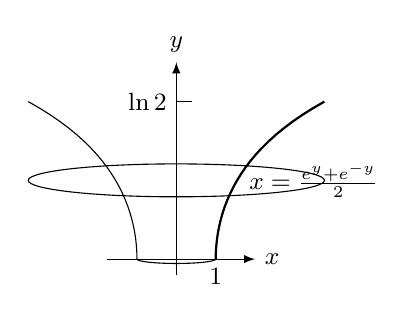
\begin{tikzpicture}[xscale=0.5,font=\small,declare function={f(\x)=1/2*(e^(\x)+e^(-\x));}]
\pgfmathsetmacro{\r}{f(2)}
\pgfmathsetmacro{\ra}{f(0)}
\pgfmathsetmacro{\ya}{ln(2)}
\draw[-latex](-1.75,0)--(2,0)node[right]{$x$};
\draw[-latex](0,-0.2)--(0,2.5)node[above]{$y$};
\draw[thick]plot[domain=0:2]({f(\x)},\x);
\draw[]plot[domain=0:2]({-f(\x)},\x);
\draw(1,0)node[below]{$1$};
\draw(0,\x) circle (\r cm and 1/18*\r cm);
\draw([shift={(180:\ra cm and 1/18*\ra cm)}]0,0) arc (180:360:\ra cm and 1/18*\ra cm);
\draw(0,2)node[left]{$\ln 2$}--++(0.4,0);
\draw(1,1)node[right,xshift=2ex]{$x=\frac{e^y+e^{-y}}{2}$};
\end{tikzpicture}
\caption{برائے سوال \حوالہ{سوال_ماورائی_سطح_طواف_رقبہ}}
\label{شکل_سوال_ماورائی_سطح_طواف_رقبہ}
\end{minipage}
\end{figure}
\ابتدا{سوال}
تفاعل \عددی{f(x)=x^2\ln\tfrac{1}{x}} کی مطلق زیادہ سے زیادہ قیمت تلاش کریں۔ یہ قیمت کہاں پائی جاتی ہے۔\\
جواب:\quad
\عددی{x=\tfrac{1}{\sqrt{e}}} پر مطلق زیادہ سے زیادہ \عددی{\tfrac{1}{2e}}
\انتہا{سوال}
%===================
\ابتدا{سوال}
تفاعل \عددی{f(x)=(x-3)^2e^x} اور اس کا ایک رتبی تفرق ایک ساتھ ترسیم کریں۔ \عددی{f'} کی قیمت اور علامت کے لحاظ سے \عددی{f} کے رویہ پر تبصرہ کریں۔ احصاء کی مدد سے ترسیم پر نمایاں نقطوں کی نشاندہی کریں۔
\انتہا{سوال}
%=====================
\ابتدا{سوال}
ربع اول میں بالائی جانب قوس \عددی{y=e^{2x}}، نچلی جانب قوس \عددی{y=e^x} اور دائیں جانب لکیر \عددی{x=\ln 3} میں محیط تکونی رقبہ تلاش کریں۔ \\
جواب:\quad
$2$
\انتہا{سوال}
%=======================
\ابتدا{سوال}
ربع اول میں بالائی جانب قوس \عددی{y=e^{x/2}}، نچلی جانب قوس \عددی{y=e^{-x/2}} اور دائیں جانب لکیر \عددی{x=2\ln 2} میں محیط تکونی رقبہ تلاش کریں۔ 
\انتہا{سوال}
%=======================
\ابتدا{سوال}
مستوی \عددی{xy} میں مبدا سے گزرتی وہ قوس  تلاش کریں جس کی لمبائی \عددی{x=0} سے \عددی{x=1} تک \عددی{L=\int_0^1\sqrt{1+\tfrac{e^x}{4}}\dif x} ہے۔\\
جواب:\quad
$y=e^{x/2}-1$
\انتہا{سوال}
%========================
\ابتدا{سوال}\شناخت{سوال_ماورائی_سطح_طواف_رقبہ}
منحنی \عددی{x=\tfrac{e^y+e^{-y}}{2},\,0\le y\le \ln 2} کو محور \عددی{y} کے گرد گھما کر سطح طواف پیدا کیا جاتا ہے (شکل \حوالہ{شکل_سوال_ماورائی_سطح_طواف_رقبہ})۔ اس سطح کا رقبہ تلاش کریں۔
\انتہا{سوال}
%========================
\ابتدا{سوال}
(ا) دکھائیں \عددی{\int\ln x\dif x=x\ln x-x+C}، (ب) وقفہ \عددی{[1,e]} پر \عددی{\ln x} کی اوسط قیمت تلاش کریں۔\\
جواب:\quad
(ا) \عددی{\tfrac{\dif}{\dif x}(x\ln x-x+C)=x\cdot\tfrac{1}{x}+\ln x-1+0=\ln x}، (ب) \عددی{\tfrac{1}{e-1}}
\انتہا{سوال}
%====================
\ابتدا{سوال}
وقفہ \عددی{[1,2]} پر \عددی{f(x)=\tfrac{1}{x}} کی اوسط قیمت تلاش کریں۔
\انتہا{سوال}
%====================
\ابتدا{سوال}\ترچھا{نقطہ $x=0$ پر $e^x$ کی خط بندی}\\
\begin{enumerate}[a.]
\item
نقطہ \عددی{x=0} پر خط بندی \عددی{e^x\approx 1+x} حاصل کریں۔
\item
وقفہ \عددی{[0,0.2]} پر \عددی{e^x} کی جگہ \عددی{1+x} استعمال کرنے سے پیدا خلل کو \عددی{5} اعشاریہ تک تلاش کریں۔
\item
وقفہ \عددی{-2\le x\le 2} پر \عددی{e^x} اور \عددی{1+x} کو ایک ساتھ کمپیوٹر پر ترسیم کریں۔ کس وقفہ پر تخمین زیادہ قیمت دیتی ہے؟  کم قیمت دیتی ہے؟
\end{enumerate}
جواب:\quad
(ب) حتمی خلل تقریباً \عددی{0.02140}
\انتہا{سوال}
%====================
\ابتدا{سوال}\شناخت{سوال_ماورائی_قواعد_قوت_نما}\ترچھا{قواعد قوت نما}\\
\begin{enumerate}[a.]
\item
مساوات \عددی{e^{x_1}e^{x_2}=e^{x_1+x_2}} جس کو اس حصہ میں حاصل کیا گیا، سے شروع کر کے دکھائیں کہ کسی بھی حقیقی عدد \عددی{x} کے لئے \عددی{e^{-x}=\tfrac{1}{e^x}} ہو گا۔ اس کے بعد کسی بھی دو اعداد \عددی{x_1} اور \عددی{x_2} کے لئے دکھائیں کہ \عددی{\tfrac{e_{x_1}}{e^{x_2}}=e^{x_1-x_2}} ہو گا۔
\item
کسی بھی دو اعداد \عددی{x_1} اور \عددی{x_2} کے لئے دکھائیں کہ \عددی{(e^{x_1})^{x_2}=e^{x_1x_2}=(e^{x_2})^{x_1}} ہو گا۔
\end{enumerate}
\انتہا{سوال}
%==================
\ابتدا{سوال}\ترچھا{$e$ کا اعشاری اظہار}\\
مساوات\عددی{\ln x=1} کو حل کرتے ہوئے \عددی{e} کی قیمت اتنے اعشاریہ تک تلاش کریں جتنے تک آپ کا کیلکولیٹر استعمال کرتے ہوئے ممکن ہو۔\\
جواب:\quad
$\num{2.71828183}$  
\انتہا{سوال}
%=====================
\ابتدا{سوال}\ترچھا{$\ln x$ اور $e^x$ کے مابین الٹ تعلق}\\
کیلکولیٹر استعمال کرتے ہوئے مرکبات \عددی{e^{\ln x}} اور \عددی{\ln(e^x)} کی قیمت تلاش کریں۔
\انتہا{سوال}
%=======================
\ابتدا{سوال}\شناخت{سوال_ماورائی_قوت_نما_تعلق_الف}
دکھائیں کہ کسی بھی عدد \عددی{a>1} کے لئے درج ذیل ہو گا (شکل \حوالہ{شکل_سوال_ماورائی_قوت_نما_تعلق_الف})۔
\begin{align*}
\int_16a\ln x\dif x+\int_0^{\ln a}e^y\dif y=a\ln a
\end{align*}
\انتہا{سوال}
%============
\begin{figure}
\centering
\begin{minipage}{0.45\textwidth}
\centering
\begin{tikzpicture}[font=\small,declare function={f(\x)=ln(\x);}]
\pgfmathsetmacro{\a}{2}
\pgfmathsetmacro{\b}{ln(\a)}
\begin{axis}[small,axis lines=middle,xlabel={$x$},ylabel={$y$},xlabel style={at={(current axis.right of origin)},anchor=west},ylabel style={at={(current axis.above origin)},anchor=south},xtick={1,\a},xticklabels={$1$,$a$},ytick={\b},yticklabels={$\ln a$},xmin=0,axis on top=true]
\fill[lgray](0,0) rectangle (\a,\b);
\addplot[domain=0.5:3]{f(x)}node[pos=0.85,left,yshift=1ex]{$y=\ln x$};
\draw(\a,0)--(\a,\b)--(0,\b);
\end{axis}
\end{tikzpicture}
\caption{ترسیم برائے سوال \حوالہ{سوال_ماورائی_قوت_نما_تعلق_الف}}
\label{شکل_سوال_ماورائی_قوت_نما_تعلق_الف}
\end{minipage}\hfill
\begin{minipage}{0.45\textwidth}
\centering
\begin{tikzpicture}[font=\small,declare function={f(\x)=\x^3;g(\x)=3.375+6.75*(\x-1.5);}]
\pgfmathsetmacro{\a}{1.2}
\pgfmathsetmacro{\b}{1.8}
\pgfmathsetmacro{\c}{1/2*(\a+\b)}
\begin{axis}[small,axis lines=middle,xlabel={$x$},ylabel={$y$},xlabel style={at={(current axis.right of origin)},anchor=west},ylabel style={at={(current axis.above origin)},anchor=south},xtick={\a,\b,\c},xticklabels={$\ln a$,$\ln b$,$\tfrac{\ln a+\ln b}{2}$},ymin=0,axis on top=true, axis y line=none]
\addplot[domain=1:2]{f(x)}node[pos=0.85,above left]{$y=e^x$};
\draw[name path=kL,dashed](\a,0)--(\a,{f(\a)})node[above]{$E$};
\draw[name path=kR,dashed](\b,0)--(\b,{f(\b)})node[above]{$F$};
\draw(\c,{f(\c)})coordinate[](kT)node[circ]{}node[below]{$M$};
\draw(\a,{f(\a)})--(\b,{f(\b)});
\addplot[domain=\a:\b]{g(x)};
\draw(\a,{g(\a)})node[left,yshift=-1ex]{$B$} (\b,{g(\b)})node[right]{$C$}  (\a,0)node[above right]{$A$}  (\b,0)node[above left]{$D$};
\end{axis}
\end{tikzpicture}
\caption{ترسیم برائے سوال \حوالہ{سوال_ماورائی_قوت_نما_تعلق_ب}}
\label{شکل_سوال_ماورائی_قوت_نما_تعلق_ب}
\end{minipage}
\end{figure}
\ابتدا{سوال}\شناخت{سوال_ماورائی_قوت_نما_تعلق_ب}\ترچھا{تکونیاتی، لوگارتھمی اور حسابی اوسط عدم مساوات}\\
\begin{enumerate}[a.]
\item
دکھائیں کہ \عددی{x} کے ہر وقفہ پر \عددی{e^x} کی ترسیم مقعر اوپر ہے۔
\item
اگر \عددی{0<a<b} ہو تب دکھائیں کہ درج ذیل ہو گا (شکل \حوالہ{شکل_سوال_ماورائی_قوت_نما_تعلق_ب})۔
\begin{align*}
e^{(\ln a+\ln b)/2}\cdot(\ln b-\ln a)<\int_{\ln a}^{\ln b} e^x\dif x<\frac{e^{\ln a}+e^{\ln b}}{2}\cdot (\ln b-\ln a)
\end{align*}
\item
جزو-ب کی عدم مساوات کو استعمال کرتے ہوئے  درج ذیل کی تصدیق کریں۔
\begin{align*}
\sqrt{ab}<\frac{b-1}{\ln b-\ln a}<\frac{a+b}{2}
\end{align*}
یہ عدم مساوات کہتی ہے کہ دو مثبت اعداد کا ہندسی اوسط ان کے لوگارتھمی اوسط سے کم ہو گا جو از خود ان کی حسابی اوسط سے کم ہو گا۔
\end{enumerate}
\انتہا{سوال}
%=========================

\حصہ{$a^x$ \, اور \, $\log_a x$}
اب تک ماسوائے \عددی{e} کے ہم نے مثبت اعداد کو غیر ناطق طاقت دینا نہیں سیکھا ہے۔ قوت نمائی تفاعل کی تعریف \عددی{e^x=\ln^{-1}x}، متغیر  \عددی{x} کی تمام حقیقی قیمتوں، ناطق اور غیر ناطق،  کے لئے درست ہے۔ اس حصہ میں ہم اس تعریف کو استعمال کر کے کسی بھی مثبت عدد کو کسی بھی ناطق یا غیر ناطق کی طاقت دینا سیکھ کر مثبت عدد \عددی{a} کے لئے قوت نمائی تفاعل \عددی{y=a^x} کی تعریف پیش کریں گے۔ اس کے ساتھ ساتھ ہم تفرق کے طاقتی قاعدہ کو حتمی شکل دیں گے (جو تمام قوت نما کے لئے درست ہو گا) اور ایک تفاعل کو دوسرے تفاعل کی طاقت دیں گے مثلاً \عددی{x^x} اور \عددی{(\sin x)^{\tan x}}، وغیرہ۔

جیسا \عددی{e^x} بہت سارے قوت نما تفاعل میں سے ایک ہے، اسی طرح \عددی{\ln x} بھی بہت سارے لوگارتھمی تفاعل،جو تفاعل \عددی{a^x} کے الٹ ہیں،  میں سے ایک ہے۔

\جزوحصہء{تفاعل $a^x$}
چونکہ کسی بھی مثبت عدد \عددی{a} کے لئے \عددی{a=e^{\ln a}} ہوتا ہے لہٰذا  ہم \عددی{a^x} کو \عددی{(e^{\,\ln a})^x=e^{\,x\ln a}} تصور کر سکتے ہیں۔ یوں ہم درج ذیل تعریف پیش کرتے ہیں۔
\begin{align}
a^x&=e^{\,x\ln a},\quad\quad a>0 &&\text{تعریف}
\end{align}

\ابتدا{مثال}
\begin{align*}
\text{(ا)}\quad 2^{\sqrt{3}}&=e^{\,\sqrt{3}\ln 2}\\
\text{(ب)}\quad 2^{\pi}&=e^{\pi\ln 2}
\end{align*}
\انتہا{مثال}
%=======================
تفاعل\عددی{a^x} قوت نما کے عمومی قواعد جنہیں جدول \حوالہ{جدول_ماورائی_قوت_نما_عمومی_قواعد} میں پیش کیا گیا ہے کو مطمئن کرتا ہے۔ ہم ان قواعد کے ثبوت پیش نہیں کریں گے۔
\begin{table}
\caption{قواعد برائے قوت نما}
\label{جدول_ماورائی_قوت_نما_عمومی_قواعد}
\centering
\renewcommand{\arraystretch}{2} 
\begin{tabular}{c|l}
\toprule
\multicolumn{2}{c}{$a>0$ ہے جبکہ $x$ اور $y$ کوئی بھی اعداد ہو سکتے ہیں}\\
\midrule
ا&$a^x\cdot a^y=a^{x+y}$\\
ب&$a^{-x}=\frac{1}{a^x}$\\
ج&$\frac{a^x}{a^y}=a^{x-y}$\\
د&$(a^x)^y=a^{xy}=(a^y)^x$\\
\bottomrule
\end{tabular}
\end{table}

\جزوحصہء{قاعدہ طاقت (حتمی صورت)}
اساس \عددی{a} کے لوگارتھم کا تفرق حاصل کرنے کی خاطر ہمیں اس کو پہلے  قدرتی لوگارتھم  کی صورت میں لکھتے ہیں۔ اگر \عددی{u} متغیر \عددی{x} کا مثبت قابل تفرق تفاعل ہو تب
\begin{align*}
\frac{\dif}{\dif x}(\log_a u)=\frac{\dif}{\dif x}\big(\frac{\ln u}{\ln a}\big)=\frac{1}{\ln a}\cdot\frac{1}{u}\frac{\dif u}{\dif x}
\end{align*}
یعنی
\begin{align}
\frac{\dif}{\dif x}(\log_a u)=\frac{1}{\ln a}\cdot\frac{1}{u}\frac{\dif u}{\dif x}
\end{align}
ہو گا۔

\ابتدا{مثال}
\begin{align*}
\frac{\dif}{\dif x}\log_{10}(3x+1)=\frac{1}{\ln 10}\cdot\frac{1}{3x+1}\frac{\dif}{\dif x}(3x+1)=\frac{3}{(\ln 10)(3x+1)}
\end{align*}
\انتہا{مثال}
%===============
\جزوحصہء{تکمل جہاں \عددی{\log_a x} پایا جاتا ہو}
جب اساس \عددی{a} کا لوگارتھم پایا جاتا ہو تب تکمل لیتے ہوئے ہم اس کو پہلے قدرتی لوگارتھم کی صورت میں بدلتے ہیں۔

\ابتدا{مثال}
\begin{align*}
\int\frac{\log_2x}{x}\dif x&=\frac{1}{\ln 2}\int\frac{\ln x}{x}\dif x&&\log_2x=\frac{\ln x}{\ln 2}\\
&=\frac{1}{\ln 2}\int u\dif u&&u=\ln x\\
&=\frac{1}{\ln 2}\frac{u^2}{2}+C\\
&=\frac{1}{\ln 2}\frac{(\ln x)^2}{2}+C=\frac{(\ln x)^2}{2\ln 2}+C
\end{align*}
\انتہا{مثال}
%===================
\جزوحصہء{اساس $10$ لوگارتھم}
اساس \عددی{10} لوگارتھم جس کو \اصطلاح{عام لوگارتھم}\فرہنگ{لوگارتھم!عام}\حاشیہب{common logarithm}\فرہنگ{logarithm!common} کہتے ہیں کئی سائنسی کلیات میں پایا جاتا ہے۔ مثال کے طور پر زلزلہ کی شدت کو عموماً اساس \عددی{10} کے  لوگارتھمی\حاشیہد{رکٹر پیمائش میں اکائی کا اضافہ حیطہ میں تقریباً \عددیء{10} گنّا  اور توانائی میں تقریباً \عددی{31.623} گنّا کا اضافہ ظاہر کرتا ہے۔} \اصطلاح{رکٹر پیمائش}\فرہنگ{رکٹر پیمائش}\فرہنگ{پیما!رکٹر}\حاشیہب{Richter scale}\فرہنگ{Richter scale} میں پیش جاتا ہے۔ رکٹر پیما کا کلیہ 
\begin{align*}
\text{شدت}\, R=\log_{10}\big(\frac{a}{T}\big)+B
\end{align*}
ہے جہاں زلزلہ پیما کے مقام پر زمینی لرزش کا حیطہ \عددی{a} ہے جس کو مائیکرو میٹر میں ناپا جاتا ہے، زلزلہ کی موج کا دوری عرصہ \عددی{T} ہے جس کو سیکنڈ میں ناپا جاتا ہے جبکہ \عددی{B} ایک تجربی جزو ہے جو مرکز زلزلہ اور زلزلہ پیما کے بیچ شدت کی کمی کو ظاہر کرتا ہے۔ 

جاپان کے شہر ناگاساکی پر گرائے  گئے ایٹمی بم میں \عددی{\SI{1.34e14}{\joule}}  توانائی تھی جو رکٹر پیما پر \عددی{5} کے برابر ہے۔  آج تک سب سے بڑا ایٹمی دھماکہ \عددی{7.1} شدت کا تھا جس میں \عددی{\SI{2.09e17}{\joule}} توانائی تھی۔  اکتوبر 8 \سن{2005} کو آزاد کشمیر میں \عددی{7.6} شدت کا زلزلہ آیا جس میں \عددی{\SI{1.585e16}{\joule}} توانائی تھی۔

\ابتدا{مثال}
مرکز زلزلہ سے زلزلہ پیما تک فاصلہ \عددی{\SI{10000}{\kilo\meter}} ہے جس کے لئے \عددی{B=6.8} ہو گا۔ مقام زلزلہ پیما پر زمین کی انتصابی حرکت \عددی{\SI{10}{\micro\meter}} اور دوری عرصہ \عددی{\SI{1}{\second}} ہیں۔ زلزلہ کی شدت تلاش کریں۔

حل:\quad
\begin{align*}
R=\log_{10}\big(\frac{10}{1}\big)+6.8=1+6.8=7.8
\end{align*}
\انتہا{مثال}
%====================
محلول کی تیزابیت\فرہنگ{تیزابیت} کو \عددی{\pH} (\اصطلاح{طاقت ہائیڈروجن})\فرہنگ{pH}\فرہنگ{طاقت!ہائیڈروجن} میں ناپا جاتا ہے جو اساس \عددی{10} کا لوگارتھمی پیمانہ\حاشیہد{$\pH$ کی جدید تعریف کے تحت اس کو "مخفی قوہ ہائیڈروجن" کہنا زیادہ بہتر ہو گا۔} ہے۔ محلول میں ہائیڈرونیم برق پارہ \عددی{[\ce{H3O^+}]} کے گھنا پن کے بالعکس کا عام لوگارتھم  اس محلول کی \عددی{\pH} قیمت ہو گی:
\begin{align*}
\pH=\log_{10}\frac{1}{[\ce{H3O^+}]}=-\log_{10}[\ce{H3O^+}]
\end{align*}
ہائیڈرونیم برق پارہ کے گھنا پن کو مول فی لٹر (\si{\mole\per\liter}) میں ناپا جاتا ہے۔تیزاب کی \عددی{\pH} قیمت \عددی{7} سے کم جبکہ القلی کی  \عددی{7} سے زیادہ ہوتی ہے۔ سرکہ کی \عددی{\pH} قیمت \عددی{3} جبکہ مقطر پانی کی \عددی{\pH} قیمت \عددی{7} ہوتی ہے۔  \عددی{\pH}  کا  پیمانہ \عددی{0} سے \عددی{14} تک ہوتا ہے۔ جدول \حوالہ{جدول_ماورائی_خوراک_ہائیڈروجن_مخفی_قوہ} میں کئی اجزاء کی \عددی{\pH} دی گئی ہے۔
\begin{table}
\caption{عمومی خوراک کی $\pH<7$ ہے۔}
\label{جدول_ماورائی_خوراک_ہائیڈروجن_مخفی_قوہ}
\centering
\begin{tabular}{rr}
\toprule
خوراک& \multicolumn{1}{c}{$\pH$}\\
\midrule
کیلا& \عددی{4.5-4.7}\\
چکوترہ& \عددی{3.0-3.3}\\
سنترا & \عددی{3.0-4.0}\\
لیموں& \عددی{1.8-2.0}\\
دودھ&\عددی{6.3-6.6}\\
مرچ&\عددی{5.1-5.7}\\
\bottomrule
\end{tabular}
\end{table}

لوگارتھم کی ایک اور مثال ڈیسی بیل \عددی{\si{\deci\bel}} پیمانہ ہے جو صدا کی بلندی کو ناپنے کے لئے استعمال کیا جاتا ہے۔ اگر صدا کی شدت \عددی{I}  واٹ فی مربع میٹر ہو تب
\begin{align}\label{مساوات_ماورائی_سطح_صدا}
\text{\RL{سطح صدا}}=10\log_{10}(I\times 10^{12})\,\si{\deci\bel}
\end{align}
ہو گا۔ جیسا اگلا مثال دکھاتا ہے، شدت صدا کو دگنا کرنے سے سطح صدا میں تقریباً \عددی{\SI{3}{\deci\bel}} کا اضافہ ہوتا ہے۔

\ابتدا{مثال}
صدا کی شدت کو دگنا کرنے سے سطح صدا میں کتنا اضافہ ہو گا؟

حل:\quad
مساوات \حوالہ{مساوات_ماورائی_سطح_صدا} کے تحت \عددی{2I} شدت صدا کے لئے 
\begin{align*}
\text{\RL{دگنی شدت کی سطح صدا}}&=10\log_{10}(2I\times 10^{12})&&\text{\RL{مساوات \حوالہ{مساوات_ماورائی_سطح_صدا} میں $2I$}}\\
&=10\log_{10}2+10\log_{10}(I\times 10^{12})\\
&=\text{\RL{اصل شدت کی سطح صدا}}+10\log_{10}2\\
&\approx \text{\RL{اصل شدت کی سطح صدا}}+3   && \log_{10}\approx 0.3
\end{align*}
ہو گا۔
\انتہا{مثال}
%======================
سطح صدا کی چند قیمتیں جدول \حوالہ{جدول_ماورائی_شدت_صدا} میں دی گئی ہیں۔
\begin{table}
\caption{سطح صدا کی چند قیمتیں۔}
\label{جدول_ماورائی_شدت_صدا}
\centering
\begin{tabular}{rr}
\toprule
سماعت کی کمتر سطح & \عددی{\SI{0}{\deci\bel}}\\
پتوں کا سرسرانا & \عددی{\SI{10}{\deci\bel}}\\
سرگوشی& \عددی{\SI{20}{\deci\bel}}\\
خاموش گاڑی& \عددی{{50}{\deci\bel}}\\
عام بات چیت& \عددی{\SI{65}{\deci\bel}}\\
تین میٹر دور ہوائی برما & \عددی{\SI{90}{\deci\bel}}\\
کانوں میں درد& \عددی{\SI{120}{\deci\bel}}\\
\bottomrule
\end{tabular}
\end{table}

